\documentclass[12pt]{article}
\usepackage[utf8]{inputenc}
\usepackage[spanish,es-tabla]{babel}
\usepackage[square,sort,comma,numbers]{natbib}
\usepackage{amssymb,amsmath,amsthm,amsfonts}
\usepackage{calc}
\usepackage{gensymb}
\usepackage{natbib}
\usepackage{url}
\usepackage{amsmath}
\usepackage{graphicx}
\usepackage{parskip}
\usepackage{fancyhdr}
\usepackage{vmargin}
\usepackage[table,xcdraw]{xcolor}
\usepackage[top=2cm,bottom=2cm]{geometry}
\usepackage{graphicx}
\usepackage{pdflscape}
\usepackage{caption}
\usepackage{subfigure}
\usepackage{xurl}

\def\BibTeX{{\rm B\kern-.05em{\sc i\kern-.025em b}\kern-.08em
    T\kern-.1667em\lower.7ex\hbox{E}\kern-.125emX}}
\setmarginsrb{3 cm}{2.5 cm}{3 cm}{2.5 cm}{1 cm}{1.5 cm}{1 cm}{1.5 cm}

\title{Ejercicio N$^{\circ}$1}					% Titulo
\author{Elias Obreque \\ Gustavo Ceballo \\ Maibeth Sánchez}					% Autor
\date{\today}						% Fecha


\makeatletter
\let\thetitle\@title
\let\theauthor\@author
\let\thedate\@date
\makeatother

\pagestyle{fancy}
\fancyhf{}
\lhead{\thetitle}
\cfoot{\thepage}

\begin{document}

%%%%%%%%%%%%%%%%%%%%%%%%%%%%%%%%%%%%%%%%%%%%%%%%%%%%%%%%%%%%%%%%%%%%%%%%%%%%%%%%%%%%%%%%%

\begin{titlepage}
	\centering
    \vspace*{0.0 cm}
    
\includegraphics[scale = 0.13]{Logo_Uchile_modern.png}\\[1.0 cm]	% Logo Universidad
    \textsc{\LARGE Universidad de Chile}\\[2.0 cm]	% Nombre Universidad
	\textsc{\Large EL7012}\\[0.5 cm]				% Codigo Curso
	\textsc{\large Control Inteligente de Sistemas, Otoño}\\[0.2 cm]		% Nombre Curso
	\rule{\linewidth}{0.2 mm} \\[0.2 cm]
	{ \huge \bfseries \thetitle}\\
	\rule{\linewidth}{0.2 mm} \\[0.5 cm]
	
	\begin{minipage}{0.4\textwidth}
		\begin{center} \large
			\emph{Autor:}\\
			\theauthor\linebreak
			\end{center}
	\end{minipage}\\[1.5 cm]
	
	{\large \thedate}\\[1.5 cm]

	\vfill
	
\end{titlepage}

%%%%%%%%%%%%%%%%%%%%%%%%%%%%%%%%%%%%%%%%%%%%%%%%%%%%%%%%%%%%%%%%%%%%%%%%%%%%%%%%%%%%%%%%%

\tableofcontents

\thispagestyle{empty}
\pagebreak
\newpage
\setcounter{page}{1}

%%%%%%%%%%%%%%%%%%%%%%%%%%%%%%%%%%%%%%%%%%%%%%%%%%%%%%%%%%%%%%%%%%%%%%%%%%%%%%%%%%%%%%%%%

\section{Introducción}

Las recientes décadas han visto un crecimiento cada vez mayor en la implementación de tecnología y robotización en industrias de diversas índoles, un reflejo de esto es la implementación de brazos robóticos en lineas de montaje, un problema bastante interesante en esta área es la trayectoria óptima de un brazo robotico entre un origen y destino dados, siendo este óptimo un parámetro medible mediante diversos factores como: un menor consumo energético, tiempo de traslado, torque involucrado, entre otros.

Intuitivamente se puede deducir que este tipo de problemas conlleva una búsqueda y optimización exhaustiva, es por esto que se hace uso de una rama de la inteligencia artificial conocida como algoritmos genéticos la cual permite que conjunto de individuos (en este caso soluciones) sean sometidos a un proceso de selección, reproducción y mutación selectiva produciendo de esta manera individuos con mejores características.

Esto es una prueba para el trabajo offline.


\section{Marco Teórico}

El problema a abordar es el siguiente: dada una posición original del brazo robotico que se  observa en la figura \ref{Brazo} es necesario calcular la trayectoria angular que deben seguir las diferentes articulaciones para alcanzar una posición objetivo mediante la aplicación de algoritmos genéticos, para estos se debe diseñar una función de fitness que además de tomar en cuenta la posición objetivo, considere una aproximación de la energía total gastada, de tal forma que las trayectorias sean cercanas a un movimiento óptimo

La implementación y funcionamiento de algoritmos genéticos junto con el método de de Denavit Hartenberg (que permite convertir el movimiento angular en trayectorias) se explican a continuación:

\begin{figure*}
\centering
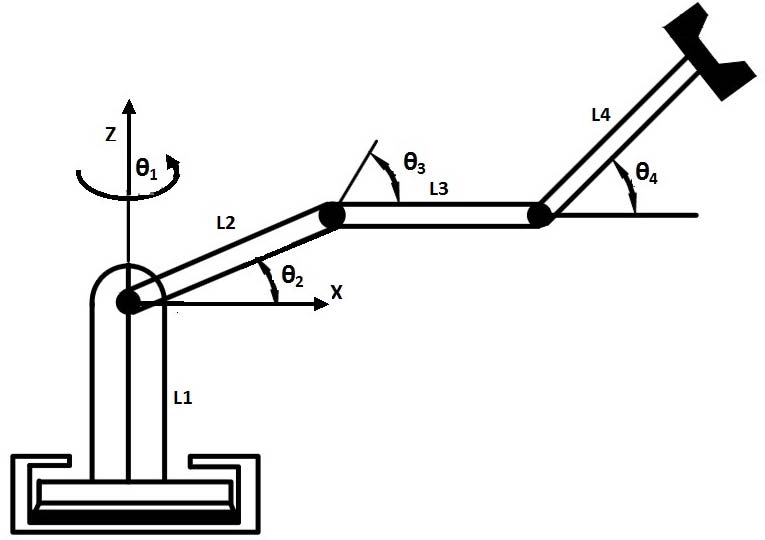
\includegraphics[width=8cm,height=5cm]{imag/Brazo.png}
\caption{Brazo robotico con 4 grados de libertad.}
\label{Brazo}
\end{figure*}

\subsection{Denavit Hartenberg}

El movimiento de cada eslabón de un brazo robótico es llamado grado de libertad, así un brazo robótico con $n$ eslabones tiene $n$ grados de libertad, si se toma cada eslabón como un elemento aislado del resto del brazo se puede apreciar que el movimiento que este hace únicamente depende de la variación angular respecto de su origen y de su longitud o sea que cualquier trayectoria del brazo robotico estará compuestas de la variación de los ángulos y longitudes de cada eslabón además de la relación entre ellos. La complejidad de este problema viene dada en que el calculo de las trayectorias posibles de un brazo compuesto de una cantidad relativamente pequeña de eslabones (3 por ejemplo) \cite{denavit-1955a} da paso a sistemas de ecuaciones de orden 32 con al menos 16 soluciones complejas. Es en este tipo de problemas que son difícilmente abordables por su complejidad matemática en donde el método de de Denavit Hartenberg (DH) sale a relucir, ya que este permite establecer la relación entre los eslabones adyacentes así como determinar la relación entre el un sistema de coordenadas origen y uno final mediante la relación entre cada par de eslabones de manera sistemática.

El primer paso es tabular los parámetros del brazo robotico, para el caso de un brazo robótico como el presentado en la sección 1 el resultado seria el de la tabla \ref{tabla1}, en donde $a_{i}$ es la longitud de cada eslabón, $\alpha_{i}$ es el ángulo entre los ejes $X$ e $Y$, $d_{i}$ representa la traslación de los eslabones respecto del eje $X$, si la coordenadas iniciales del primer eslabón están en el origen cartesiano (0,0,0) y no hay traslación en el eje $X$ entonces sera 0 para todos los eslabones y finalmente $\theta_{i}$ es el ángulo conformado entre $X$ y $Z$.

\begin{table}[]
\centering
\caption{Parametros de DH}
\begin{tabular}{|c|c|c|c|c|}
\hline
\textbf{Eslabon(i)} & \textbf{$a_{i}$} & \textbf{$\alpha_{i}$} & \textbf{$d_{i}$} & \textbf{$\theta_{i}$} \\ \hline
\textbf{1} & \textit{0} & \textit{90º} & \textit{0} & \textit{$\theta_{1}$} \\ \hline
\textbf{2} & \textit{$L_{2}$} & \textit{0} & \textit{0} & \textit{$\theta_{2}$} \\ \hline
\textbf{3} & \textit{$L_{3}$} & \textit{0} & \textit{0} & \textit{$\theta_{3}$} \\ \hline
\textbf{4} & \textit{$L_{4}$} & \textit{0} & \textit{0} & \textit{$\theta_{4}$} \\ \hline
\end{tabular}
\label{tabla1}
\end{table}

El segundo paso es el calculo de la matriz $A$ por cada uno de los eslabones, su notación es $_{i-1}^{i}A$ y representa la relación de cada articulación con la anterior, ecuación \eqref{matriz DH}, en donde $c$ y $s$ son coseno y seno respectivamente y los índices se reemplazan por los componentes de la Tabla \ref{tabla1}:

\begin{gather}
    _{i-1}^{i}A
    =
    \begin{bmatrix}
        c\theta_{i} & -s\theta_{i}c\alpha_{i}	& s\theta_{i}s\alpha_{i}	& a_{i}c\theta_{i}  \\
        s\theta_{i} & c\theta_{i}c\alpha_{i} 	& -c\theta_{i}s\alpha_{i}	& a_{i}s\theta_{i}  \\
        0           & s\alpha_{i} 				& c\alpha_{i} 				& d_{i} \\
        0           & 0 & 0 & 1 \\
    \end{bmatrix}
    \label{matriz DH}
\end{gather}

Finalmente y para obtener las coordenadas cartesianas fruto de la relación entre el eslabón de origen con cualquier otro es necesario obtener la matriz homogénea $T$, para esto se multiplican la matrices $A$ como se observa en la ecuación \eqref{Matriz T ultima} en donde las coordenadas cartesianas en 3D son $d_{x}$, $d_{y}$ y $d_{z}$, los otros parámetros $d_{i}$ junto con $r_{i}$ están asociados a la rotación y el resto a la perspectiva.

\begin{gather}
    _{0}^{i}T = \prod_{j=1}^{i} ( _{j}^{j-i}\textrm{A})=
    \begin{bmatrix}
        r_{11}	& d_{12}	& d_{13}	& d_{x}     \\
        r_{21} 	& d_{22}	& d_{23}	& d_{y}     \\
        r_{31}	& d_{32}	& d_{33}	& d_{z}     \\
        0		& 0         & 0         & 1         \\
    \end{bmatrix}
    \label{Matriz T ultima}
\end{gather}


\subsection{Algoritmos Genéticos}

Los algoritmos genéticos han nacido como herramienta para la optimización y solución de problemas en los que sus parámetros son difícil de calcular de forma analítica. Un ejemplo claro de esto son los problemas no lineales de fenómenos físicos, problemas para el cual ya se han desarrollado herramientas resolutivas \cite{ghodousian_efficient_2018}. El trasfondo del algoritmo genético se basa en crear un conjunto inicial de posibles soluciones (que puede ser expresada en un valor real o binario según corresponda el problema) y luego es evaluada en la función característica del problema.

Dependiendo del tipo de problema se pueden presentar dos escenarios: cuando se define un conjunto de valores de referencias a la que la función característica debe alcanzar como posición, velocidad, temperatura, presión, etc; o cuando simplemente se desea escoger el conjunto de solución que maximiza (minimiza) un término, por ejemplo, el empuje de motor. Este conjunto de solución posibles se evalúa por medio una función fitness (a definir por el usuario) que permite decidir cuantitativamente que valores de la solución fue más acertada.

Los mejores conjuntos solución irán evolucionando mediante avanzan en el tiempo (o número de generaciones) y crearan nuevos conjuntos que tendrán las propiedades de las generaciones pasados más favorables. Dependiendo de la rapidez con la que evoluciona la solución, se pueden aplicar técnicas de algoritmos genéticos para solucionar problemas de control robusto de alto grado de dificultad como sistemas no lineales \cite{noauthor_robust_nodate}. Otro ejemplo cercano al problema mencionado en este proyecto se encuentra en \cite{gonzalez_cinematica_2015} y \cite{momani}  donde se busca solucionar la dinámica de un brazo robótico con algoritmo genético y explicando el uso de la dinámica inversa. El proceso evolutivo se presenta en el diagrama general de la Figura \ref{genetico}. \\

Para representar las soluciones en algoritmo genético se presentan las siguientes definiciones las cuales estan de acorde al problema presentado:
\begin{itemize}
    \item Generación: Conjunto de trayectorias de $G$ brazos independientes.
    \item Individuo: Trayectoria de cada brazo producto del movimiento de los eslabones que lo componen, denotado como $I$.
    \item Gen: Trayectoria individual de un eslabón denotado como $g$.
    \item Cromosoma: Cada uno de los $k$ puntos cuyo conjunto representa la trayectoria de cada eslabón, denotado como $i$.
\end{itemize}

\begin{figure*}
\centering
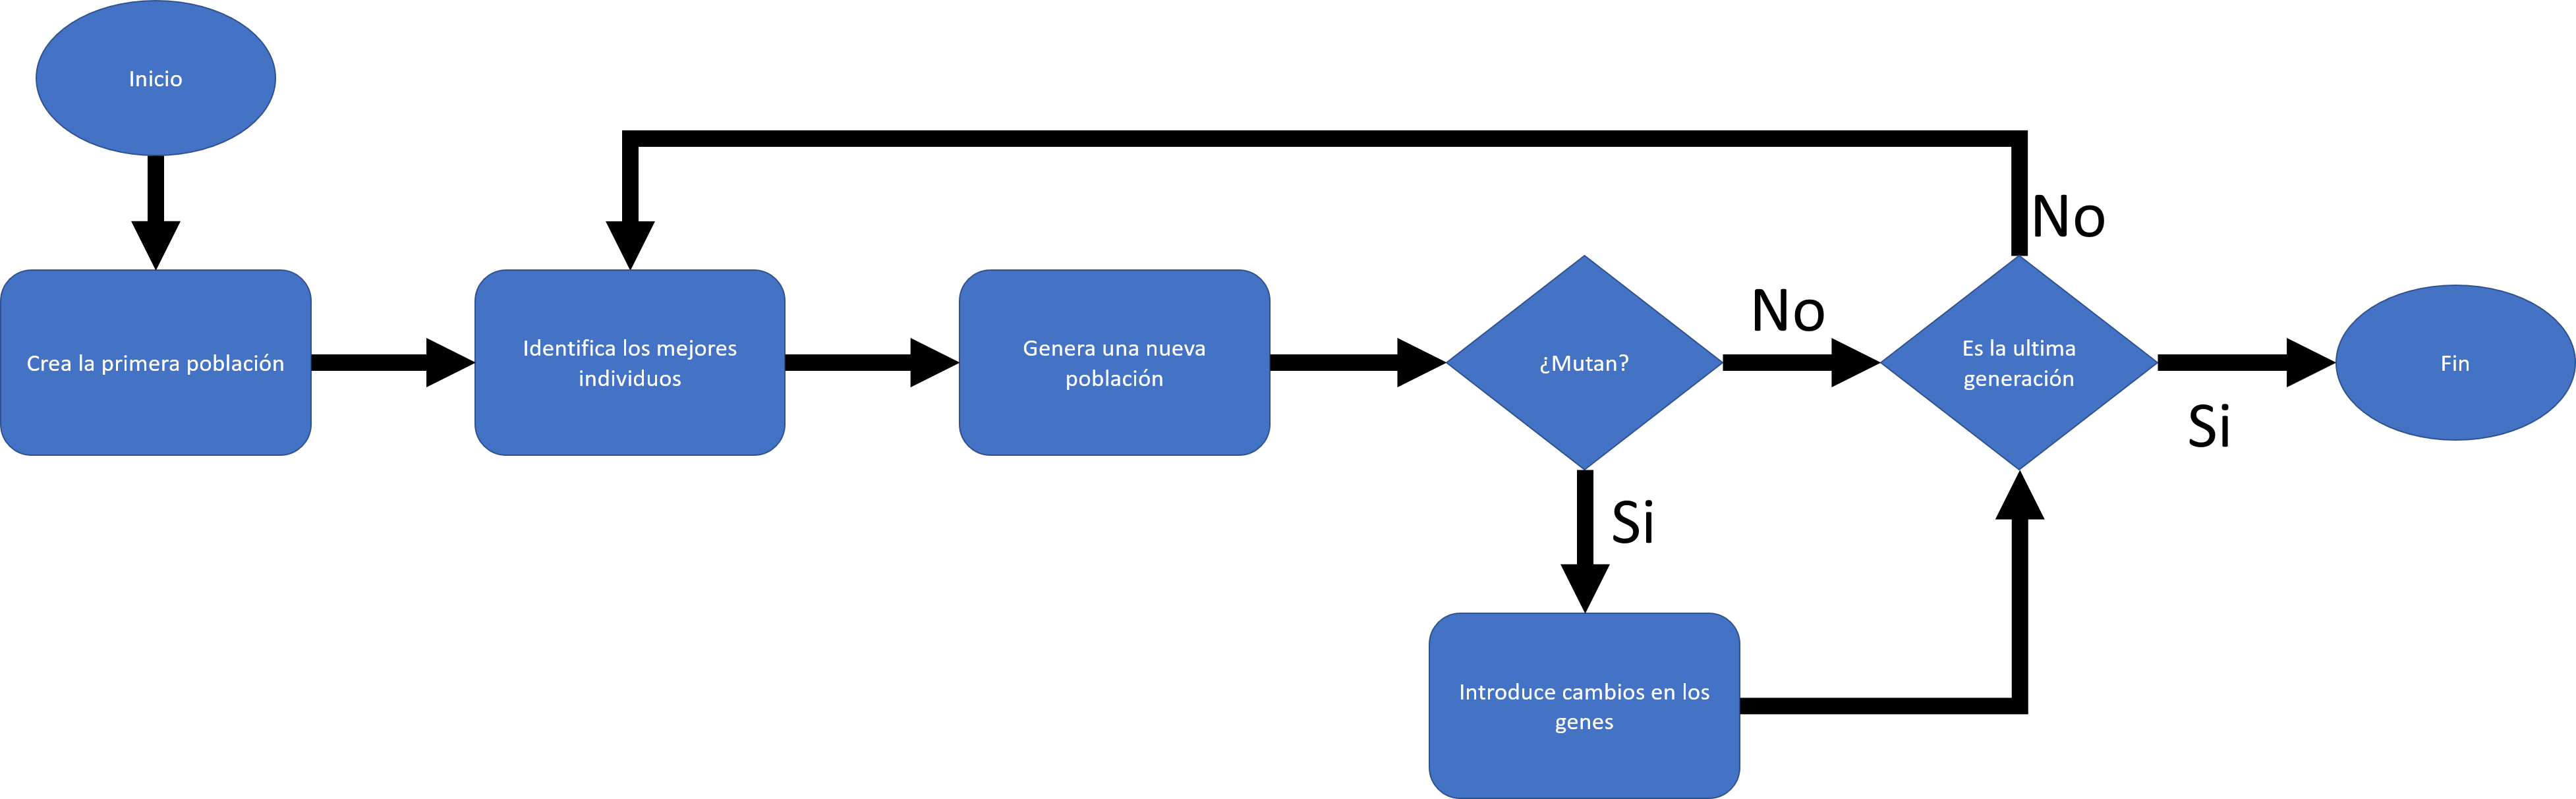
\includegraphics[width=13cm,height=5cm]{imag/Algortimo_Genetico_diagrama.png}
\caption{Diagrama de algoritmo genético.}
\label{genetico}
\end{figure*}




\subsubsection{Creación de los individuos de la Población Original}

El gen asociado a una articulación se crea según lo visto en ecuación \eqref{eqgen}, en donde $\theta _{inicial}$ y $\theta _{final}$ representan los ángulos máximos y mínimos en los cuales el brazo realiza su movimiento, permite que la población inicial presente una trayectoria cercana a la solución deseada, si bien no óptima. Por otra parte la ecuación \eqref{eqpesos} es una función tangente hiperbolica con limites entre [0,1] que en fondo establece el comportamiento de cada articulación, en donde:

\begin{itemize}
\item $i$ representa cada cromosoma siendo sus limites $ 2\leq i \leq i_{k}-1$ con $i_{k}$ siendo la cantidad de cromosomas.
\item $\mu$ variable aleatoria con limites $1\leq \mu  \leq i_{k}$.
\item $\sigma$ variable aleatoria con limites $1\leq \sigma\leq i_{k}/6$.
\end{itemize}

\begin{equation}
Gen(i)=\theta _{inicial}+(\theta _{final} - \theta _{inicial})*W(i)
\label{eqgen}
\end{equation}

\begin{equation}
W(i)=\frac{1}{2}\left [ 1+tanh  \left ( \frac{i- \mu} {\sigma} \right ) \right ]
\label{eqpesos}
\end{equation}

Ya que la ecuación \eqref{eqpesos} tiene una componente aleatoria, al utilizar esta en la ecuación \eqref{eqgen} para la creación de los genes de cada individuos, hace mas probable tener distintas trayectorias. El como esto se represan tabularmente se puede observar en la tabla \ref{tablagenes} en donde se tiene como los $i_{k}$ cromosomas asociados a cada uno de los genes varían dentro del rango de un $\theta _{inicial}$ de $0\degree$ hasta un $\theta _{final}$ de $90\degree$.


\begin{table}[]
\centering
\caption{Representación tabular de un individuo.}
\begin{tabular}{c|c|c|c|c|c|c|}
\cline{2-7}
\multicolumn{1}{l|}{} & \multicolumn{6}{c|}{\textbf{Cromosomas {[}Grados{]}}} \\ \hline
\multicolumn{1}{|c|}{\textbf{Gen/Eslabón}} & \textbf{1} & \textbf{2} & \textbf{3} & \textbf{4} & \textbf{...} & \textbf{$i_{k}$} \\ \hline
\multicolumn{1}{|c|}{\textbf{1}} & 0 & 1,42-11 & 3,38e-11 & 6,10e-11 & ... & 87.15 \\ \hline
\multicolumn{1}{|c|}{\textbf{2}} & 0 & 1,87 & 4,03 & 6,50 & ... & 90 \\ \hline
\multicolumn{1}{|c|}{\textbf{3}} & 0 & 0 & 0 & 0 & ... & 79.87 \\ \hline
\multicolumn{1}{|c|}{\textbf{4}} & 0 & 2,57e-05 & 5,41e-05 & 9,79e-05 & ... & 89.99 \\ \hline
\end{tabular}
\label{tablagenes}
\end{table}
Una vez se tienen todos los individuos de la población original, cada uno con sus genes y cromosomas correspondientes es necesario traducir este movimiento angular en coordenadas cartesianas, por lo cual se hace uso del método DH explicado en la sección 2.1, a partir de esto se obtiene la trayectoria de los k individuos de la generación en 3 dimensiones.

\subsubsection{Fitness}
El fitness escogido relaciona el punto geométrico objetivo con el punto en el cual se encuentra la punta del brazo y la velocidad lineal del brazo en cada paso. Utilizando el método de Denavit Hartenberg se obtiene la posición cartesiana del brazo y se calcula la norma del vector diferencia denominado como $E$. De esta forma se puede penalizar el cumplimiento de la posición objetivo cambiando su peso al multiplicar $E$ por un factor de ganancia $\beta$.\\
Para penalizar la distancia que hay de una muestra a otra (distancia entre cromosomas) que llamaremos \textit{smoothness} se penaliza la velocidad de traslación de las muestras. Para ello, se calcula la velocidad de cada individuo en sus respectivos pasos, luego, se escoge la máxima velocidad de traslación de cada engranaje. Finalmente, se define $V$ como la media de las velocidades máximas de cada engranaje. Este término también es multiplicado por una ganancia $\alpha$ de tal forma que la penalización de $V$ tenga una correspondencia con $E$, es decir, se impone que $\beta$ es el complemente de $\alpha$ ($\alpha + \beta = 1$).

Un caso que refleja un \textit{smoothness} ($V$) demasiado alto se observa en la figura \ref{smoothness}, en donde se tiene que no existe una distancia consistente entre los diferentes cromosomas que conforman un gen en particular, concentrándose estos en los bordes.

\begin{equation}
    Fitness = \frac{1}{1 + \beta E + \alpha V}
    \label{fitness}
\end{equation}

\begin{figure*}
\centering
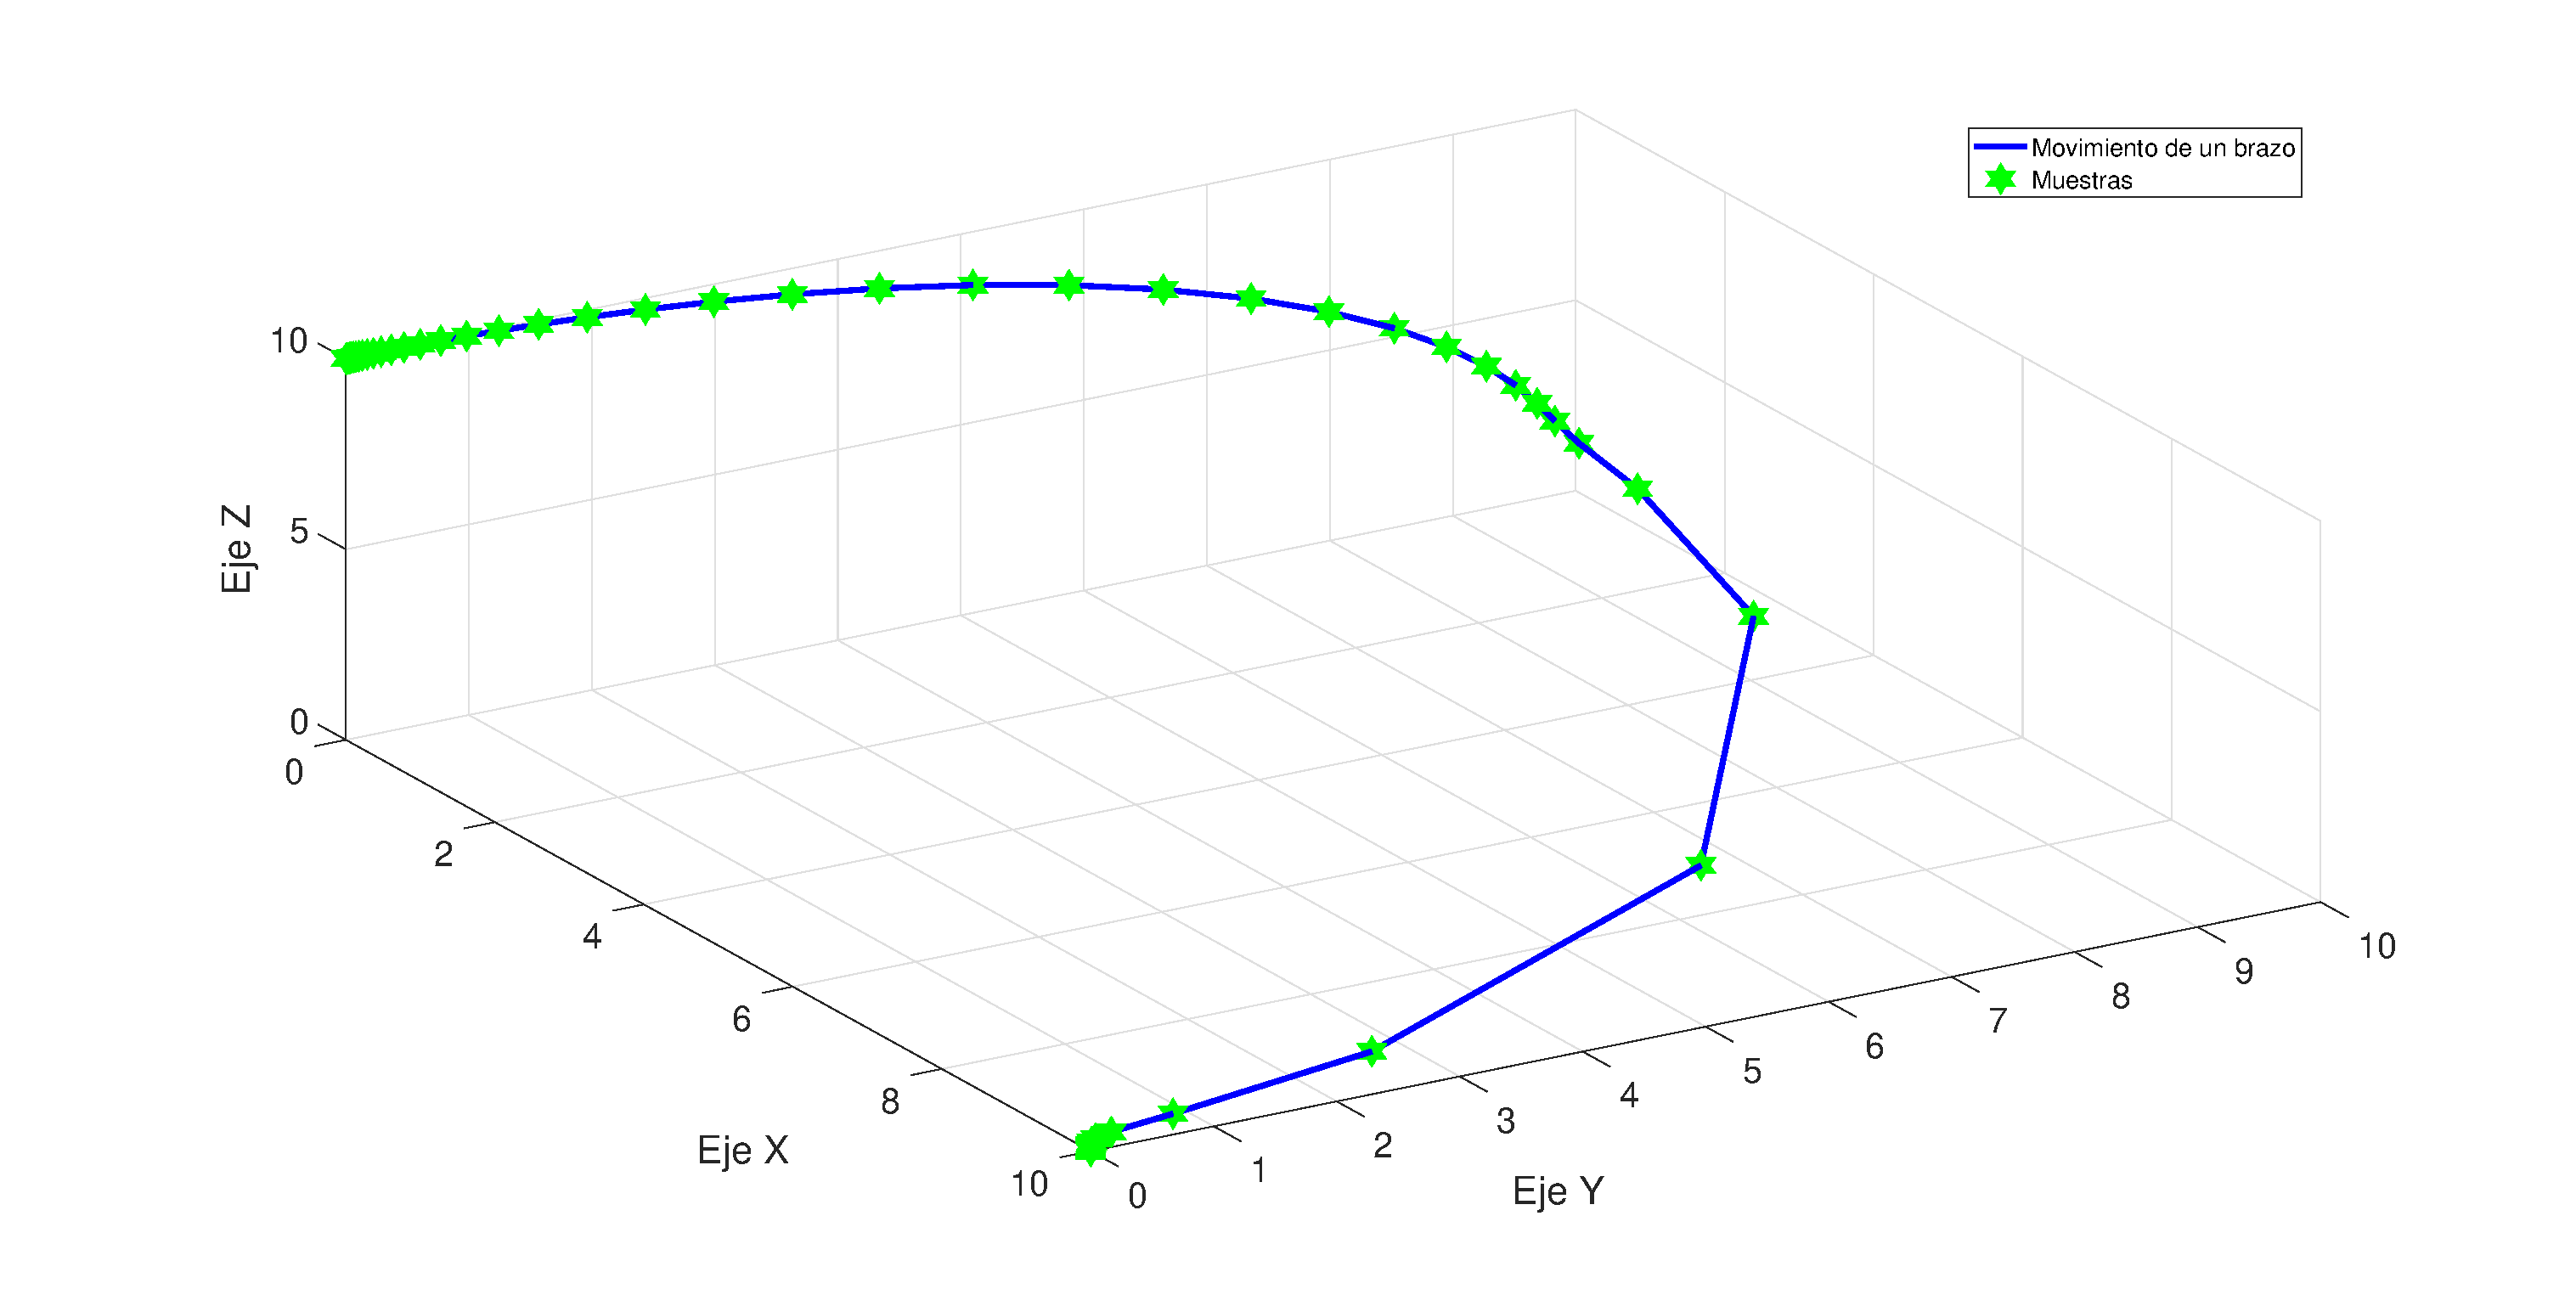
\includegraphics[width=8cm,height=5cm]{imag/EjemploSmoothness.eps}
\caption{Trayectoria de un brazo mediante los puntos de muestreo.}
\label{smoothness}
\end{figure*}

%figura \ref{tangente}
%\begin{figure}
%\centering
%\subfigure[Resultado de la función para distintas medias y sigmas aleatorios.]{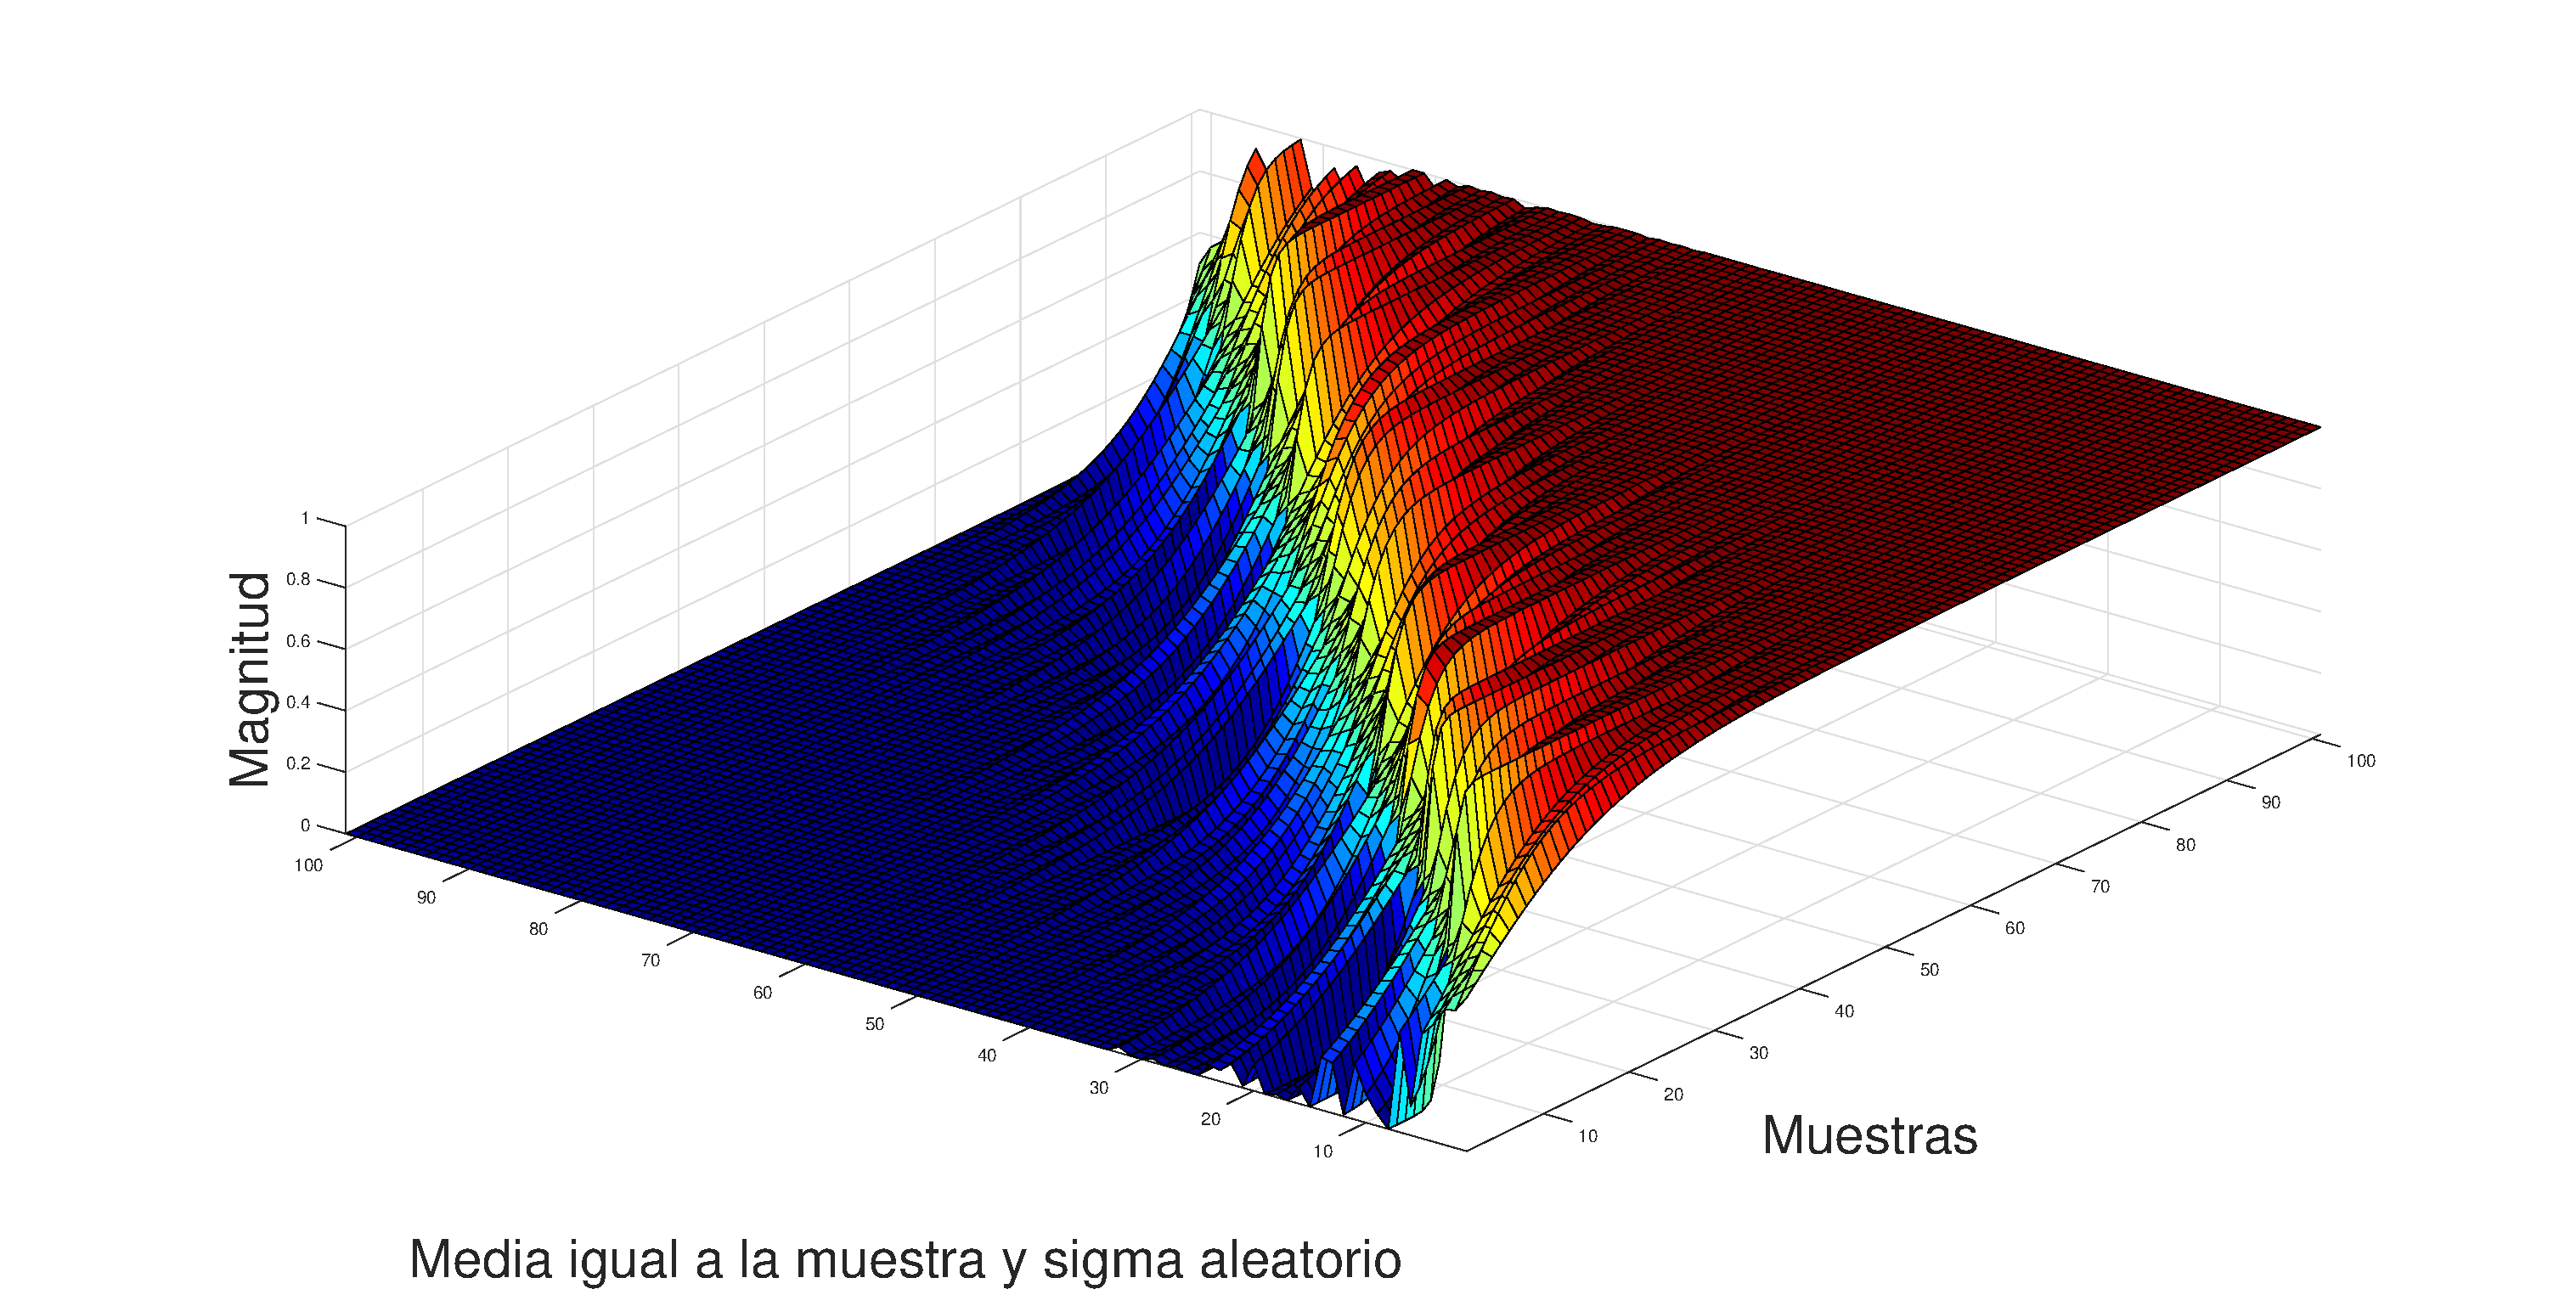
\includegraphics[width=7cm,height=4cm]{imag/FuncionTangenteHiperbolica3D.eps}}
%\subfigure[Muestra de las funciones.]{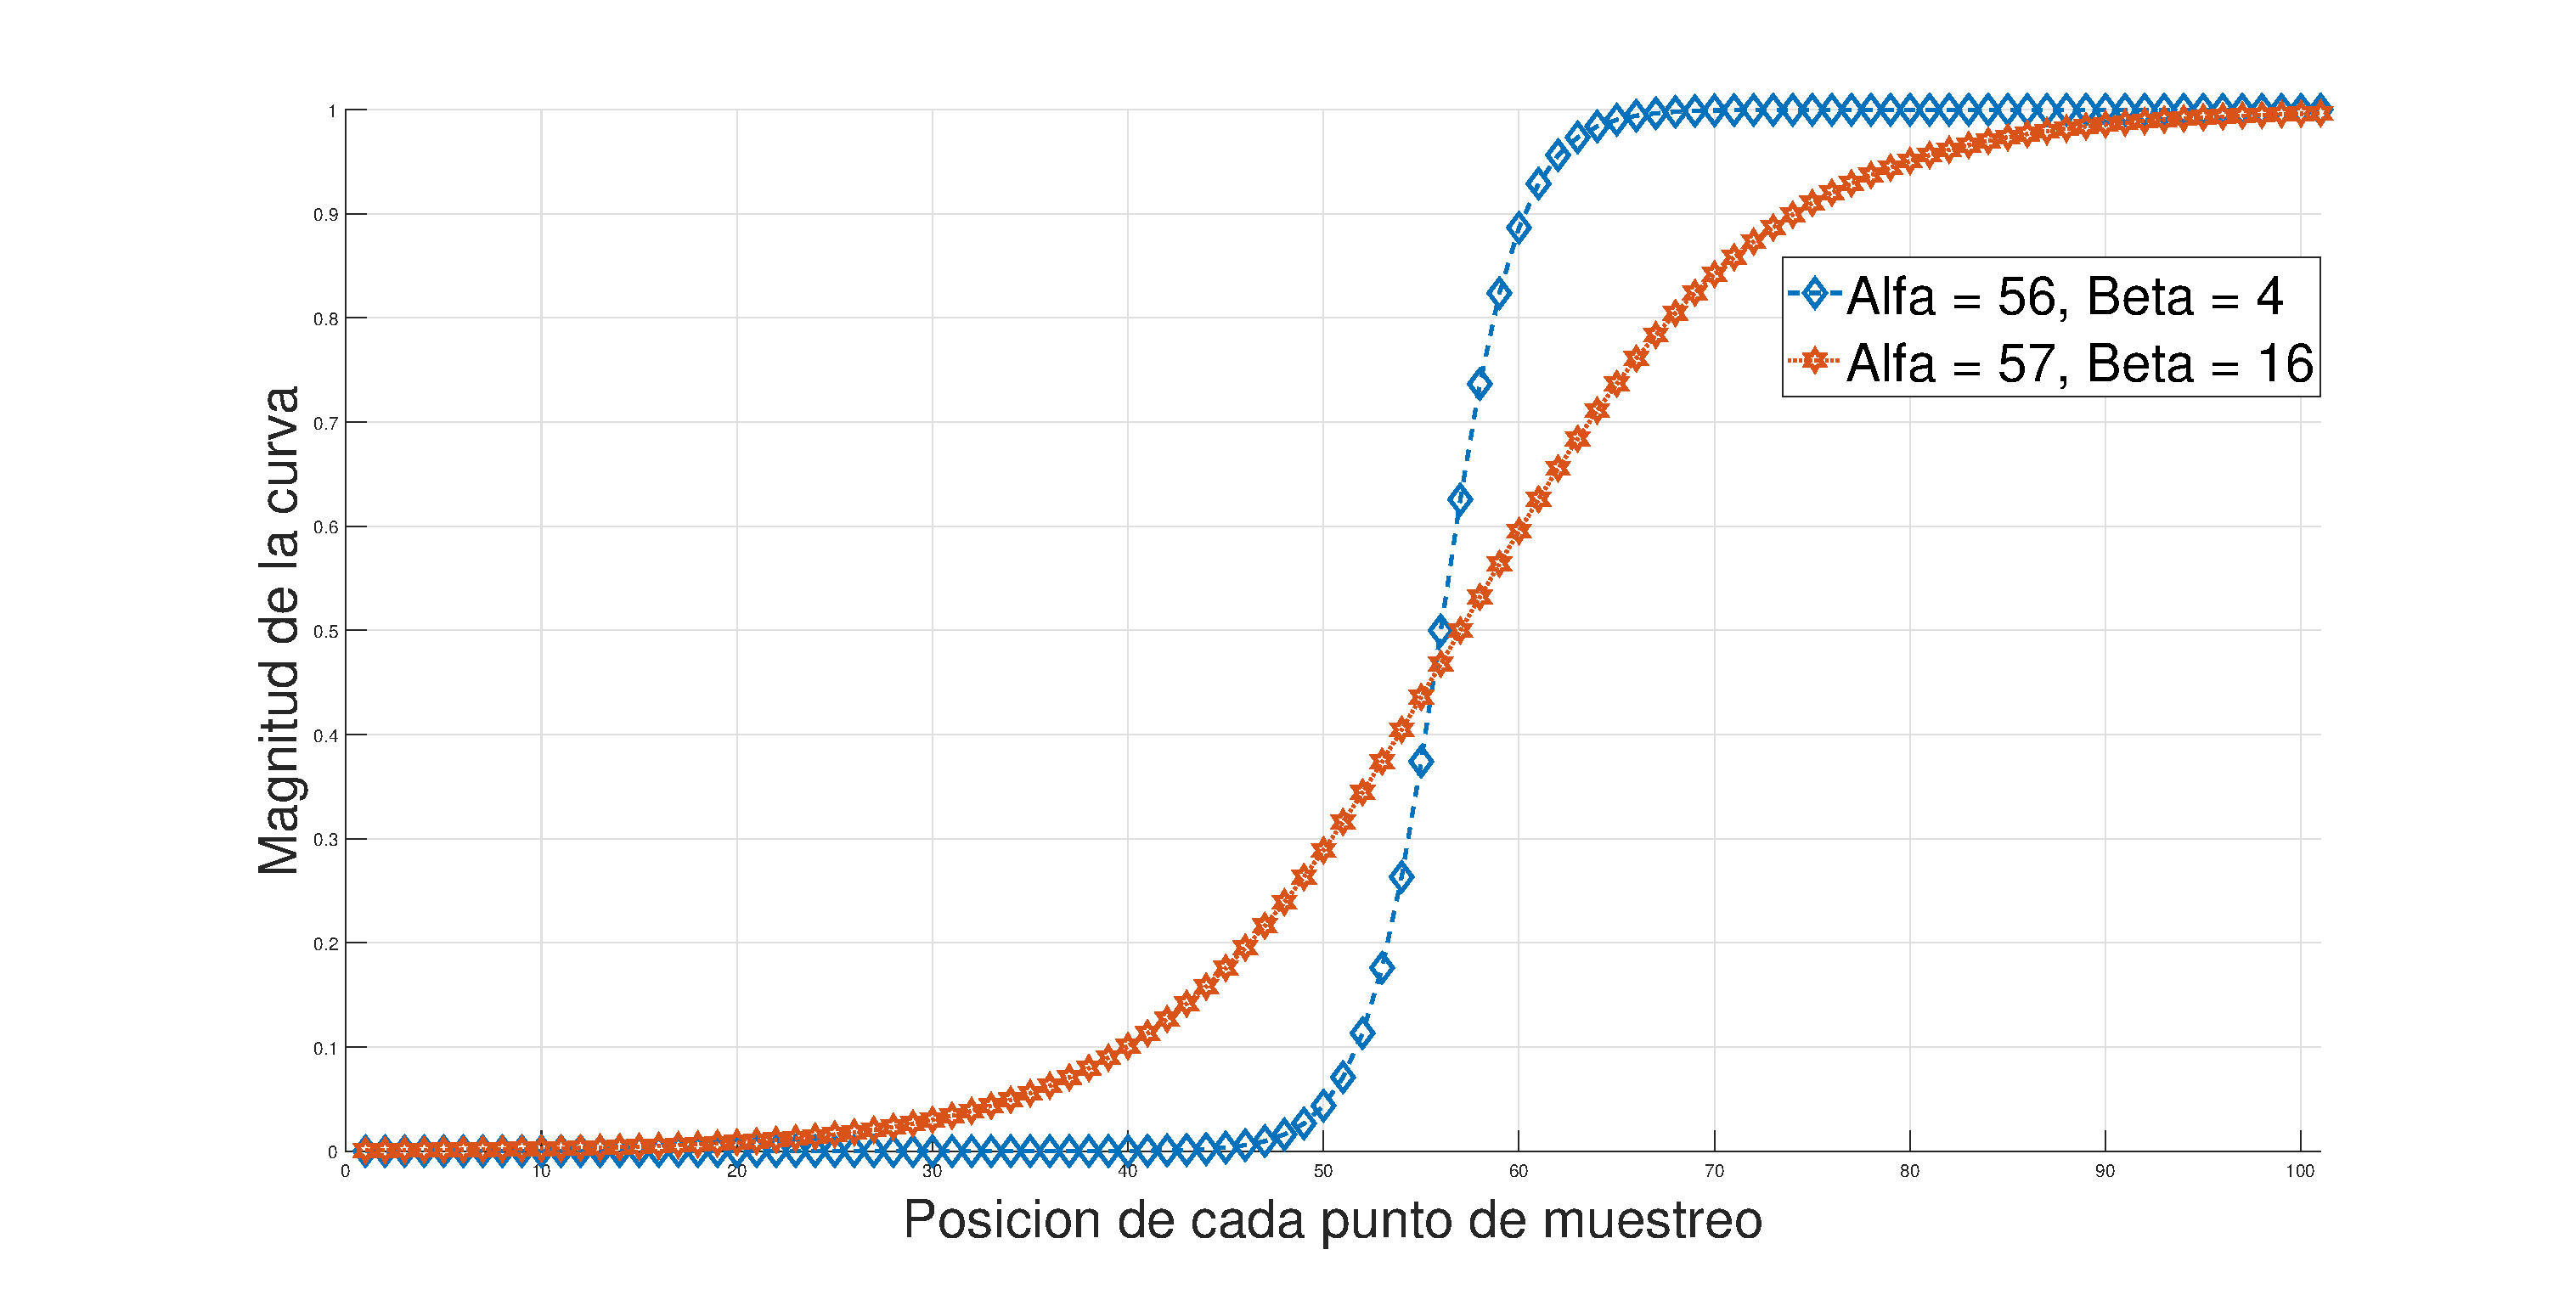
\includegraphics[width=7cm,height=4cm]{imag/funcionestangentehiperbolica.eps}}
%\caption{Comportamiento de la función tangente hiperbólica.}
%\label{tangente}
%\end{figure}



\subsubsection{Selección de los individuos}

Es necesario obtener una cantidad de pares de individuos igual a (cantidad de individuos de la generación)/2 ya que estos son los que darán paso a la nueva generación en el crossover, para realizar esto se sigue el siguiente procedimiento:

Como una forma de asegurar que un \% de los individuos con mejor fitness sean parte de los padres de la nueva generación es que se selecciona el 10\% de la población con el mejor fitness, o sea la elite de la generación, y se ordenan de a pares.

Con el 90\% restante se realiza un torneo, eso significa que se toman de a pares y se selecciona a quien tenga mejor fitness descartando al otro, luego se toman los individuos ganadores del torneo y se ordenan de a pares, ya que con esto faltaran parejas estas se obtienen a partir de las permutaciones faltantes de quienes ganen el torneo.

Finalmente los pares de padres de la elite de la generación y los pares obtenidos mediante el torneo se unen para posteriormente ser utilizados en el proceso del crossover.


\subsubsection{Crossover y mutación}

En este paso se toma cada pares de padres obtenidos en el paso anterior y se identifican como $Padre1$ y un $Padre2$, la creación de cada par de hijos se hace según la ecuación \eqref{hijos}, en donde la cantidad de genes de cada individuo se representa como $h$ y $W$ corresponde a la ecuación \eqref{eqpesos}, en el fondo la ecuación \eqref{eqpesos} funciona como un peso que se multiplica por los cromosomas de un padre y el complemento del peso por el padre restante, consiguiendo de esta manera un hijo que aúna parte de los cromosomas de cada uno de los progenitores.

\begin{align}
Hijo1(i,h) = Padre1(i,h)*W(i,h)+Padre2(i,h)*\left[1-W(i,h)\right]  \nonumber \\
Hijo2(i,h) = Padre2(i,h)*W(i,h)+Padre1(i,h)*\left[1-W(i,h)\right]
\label{hijos}
\end{align}

Es aquí en donde es relevante la introducción de las mutaciones ya que permite introducir cambios a corto, mediano y largo plazo en las poblaciones, para esto se utiliza la ecuación \eqref{muta}, en donde $d$ esta en el rango entre $[\mathrm{min}(Hijo(h,i)) - \mathrm{max}(Hijo(h,i)),\ \mathrm{max}(Hijo(h,i)) - \mathrm{min}(Hijo(h,i))]$, $M$ es una función de mutación gaussiana que varía de 0 a 1 definida en la ecuación \eqref{gauss} cuyos $\mu$, $\sigma$ e $i$ son los mismos que se utilizan en el proceso del crossover (ecuación \eqref{hijos}).

\begin{equation}
HijoMutado(h,i) = Hijo(h,i)+d*M(h,i)
\label{muta}
\end{equation}

\begin{equation}
M(h,i)=\exp\left(\frac{-(i-\mu)^{2}}{2\sigma^{2}}\right)
\label{gauss}
\end{equation}

Algunas mutaciones pueden dar paso a situaciones en las cuales los genes muestran comportamientos que se salen demasiado de lo esperado, en este caso es necesario limitar estos comportamientos acotándolos inferior y superiormente llamándose esto método \textit{Fixed Limit}.

Un ejemplo de todo lo anteriormente nombrado se puede observar en la figura \ref{esteeee}, en donde en \ref{aaa1} se tiene el proceso de crossover y en \ref{aaa2} como un hijo cualquiera sufre una mutación y luego se le aplica el método \textit{Fixed Limit},

\begin{figure}
\centering
\subfigure[Cruza entre 2 individuos.]{\label{aaa1}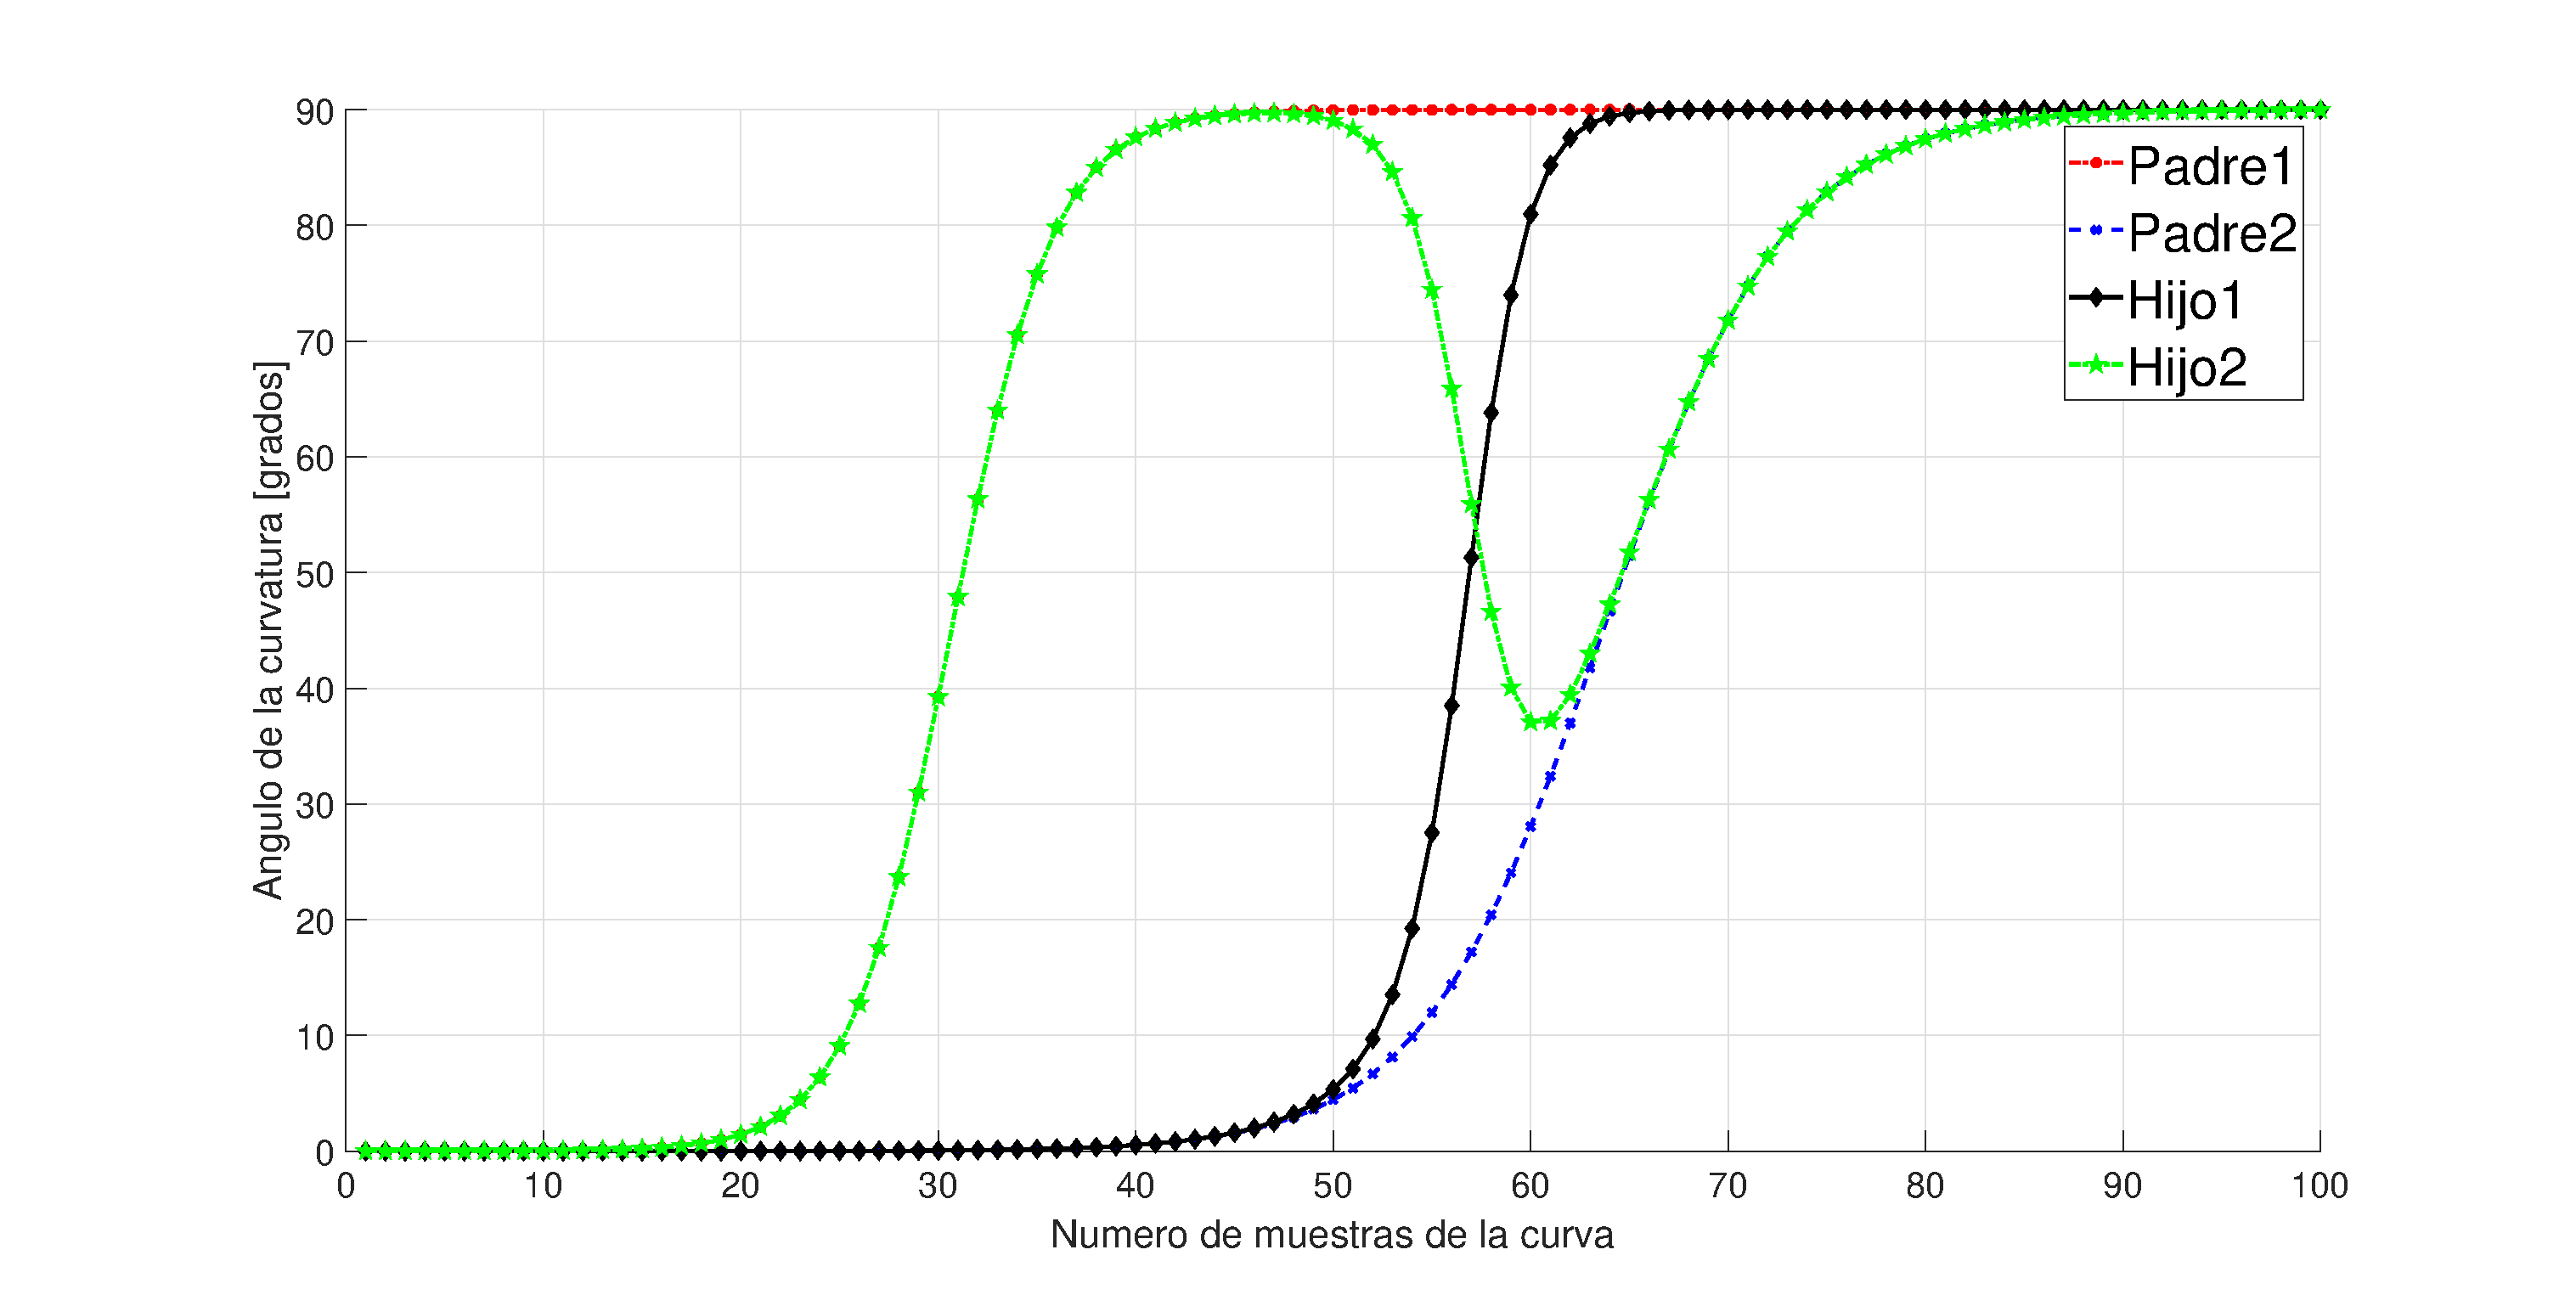
\includegraphics[width=7cm,height=5cm]{imag/Crossover.eps}}
\label{esteeee1}
\subfigure[Regulación de la mutación mediante fixed limit.]{\label{aaa2}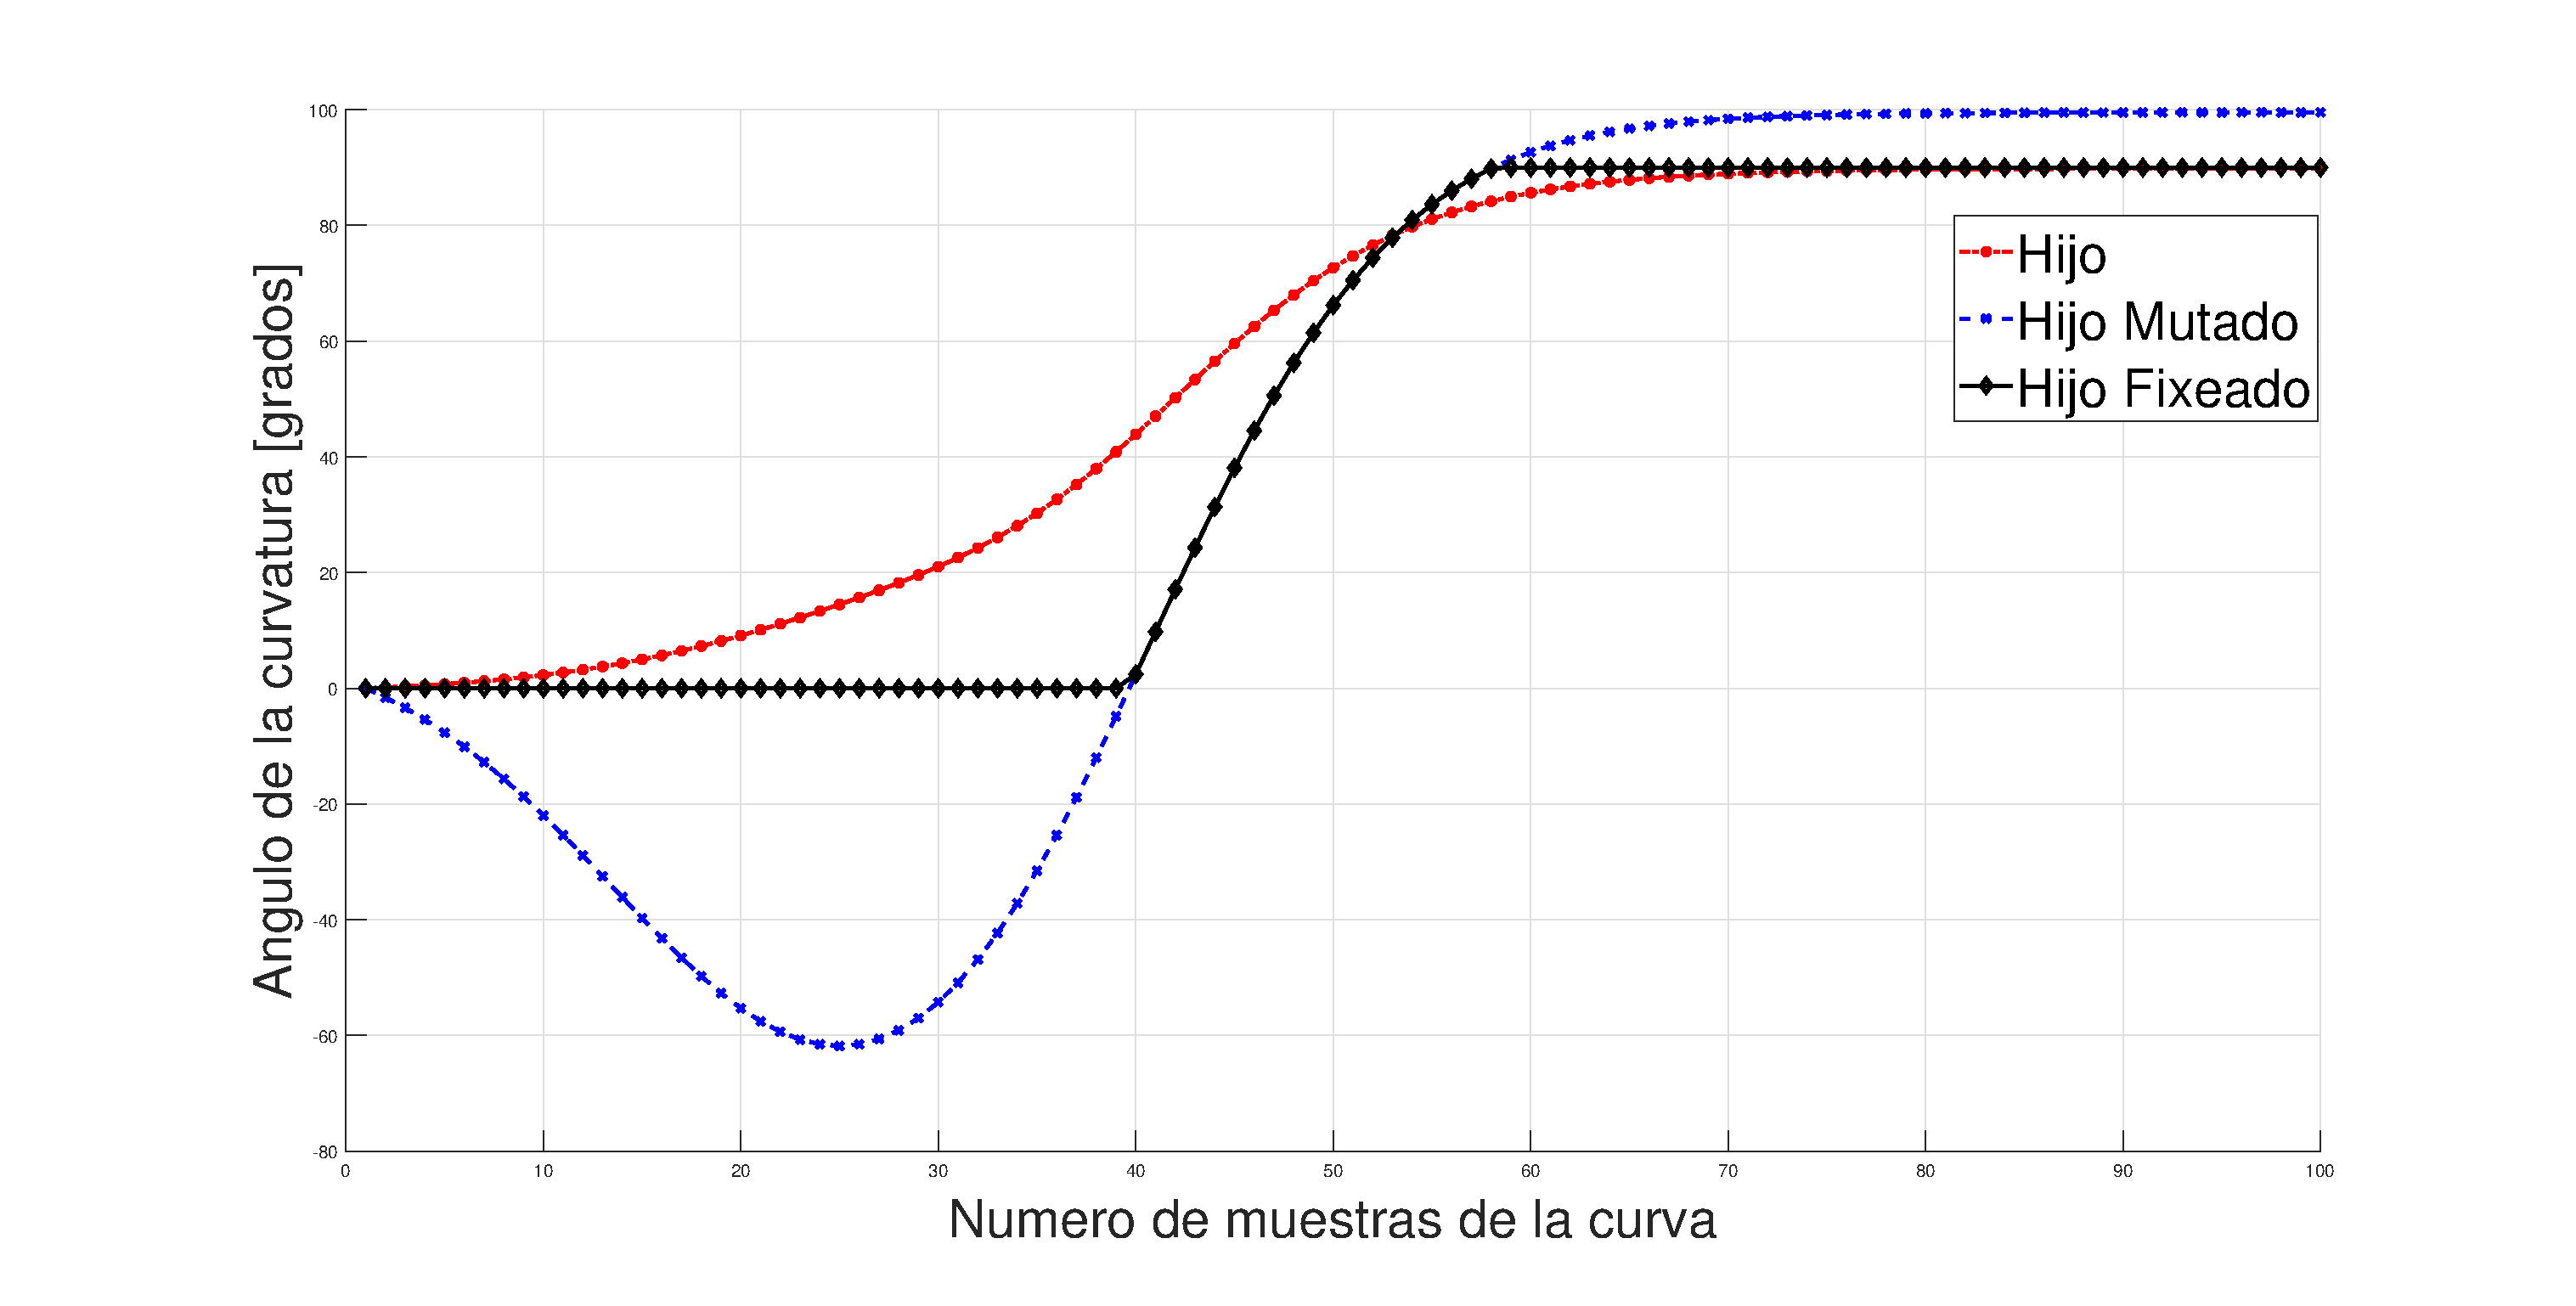
\includegraphics[width=7cm,height=5cm]{imag/MutacionFix.eps}}
\label{esteeee2}
\caption{Crossover y mutación.}
\label{esteeee}
\end{figure}




\section{Metodología}

El desarrollo de la solución se crea en ambiente Matlab debido a la familiaridad con el lenguaje y la ductilidad que este entrega en la implementación de soluciones, donde uno de los subconjunto es implementado para conocer la ubicación en coordenadas cartesianas de cada muestra por medio de la matriz de Denavid Hartenberg. El uso de algoritmo genético, la creación de los primeros individuos, la ebulición, selección, crossover y mutación se presentaran con más detalles en el mismo capitulo.

Para visualizar los resultados se presentan 3 link dispuestos desde el origen que presentan las movimientos de 3 de los 4 engranajes. El último engranaje se encuentra en el origen y permite la rotación en el eje Z.

No se utiliza una base de datos ya que la población inicial se genera mediante la ecuación \eqref{eqpesos} en donde es particularmente importante la ecuación \eqref{eqgen} la cual es una función aleatoria uniformente distribuida entre 0 y 1, siendo esta misma la que interviene en el proceso de crossover.

El código (creado en su totalidad por los autores del informe) y las instrucciones para su ejecución esta disponible en  \url{https://github.com/EliasObreque/EL4106} \cite{GIT}, los parámetros utilizados en la simulación están tabulados en la tabla \ref{parametros} y el tiempo de simulación en un notebook con las características descritas en \cite{gp62} es de aproximadamente 20 minutos. El código esta seteado para entregar los resultados de una semilla en particular la cual puede ser configurada mediante el parámetro rng de Matlab.


\begin{table}[]
\centering
\caption{Parámetros de la simulación.}
\begin{tabular}{|l|l|}
\hline
\textbf{Parámetro} & \textbf{Valor} \\ \hline
\textit{\textbf{Generaciones}} & 80 \\ \hline
\textit{\textbf{Individuos}} & 200 \\ \hline
\textit{\textbf{Cromosomas}} & 100 \\ \hline
\textit{\textbf{Genes}} & 4 \\ \hline
\textit{\textbf{Probabilidad de mutación}} & 0.1 \\ \hline
\textit{\textbf{$\alpha$}} & 0.5 \\ \hline
\textit{\textbf{$\beta$}} & 0.5 \\ \hline
\end{tabular}
\label{parametros}
\end{table}


\subsection{Selección de los hiperparámetros de fitness}

Como se ha mencionado en la sección 2.2.2 es necesario definir el peso de $\alpha$ y $\beta$ de tal manera de que sean lo suficientemente representativos del real estado de la generación, a modo de recordatorio lo que representa cada uno de ellos:

\begin{itemize}
    \item $\alpha$ regula el \textit{smoothness} de las curvas o sea la velocidad de traslación de las muestras o cromosomas.
  \item $\beta$ regula el error de posición o sea la distancia cartesiana entre las coordenadas deseadas y las coordenadas a las cuales se llego
\end{itemize}

El resultado de variar $\alpha$ y $\beta$ con los mismos parámetros de la tabla \ref{parametros} se puede observar en la figura \ref{muchas}, en este caso se considera una población con mutaciones. En \ref{this1} se tiene el error de posición para cada una de estas variaciones, queda claro que para alfas cada vez mas grandes el error de posición aumenta, en \ref{this2} refleja como el promedio del fitness evoluciona con cada generación, siendo particularmente alto para un $\beta$ y un $\alpha$ cada vez mayor y menor respectivamente, en \ref{this3} se tiene que el mejor fitness de la generación sigue la misma tendencia.

\begin{figure}
\centering
\subfigure[Error de posición]{\label{this1}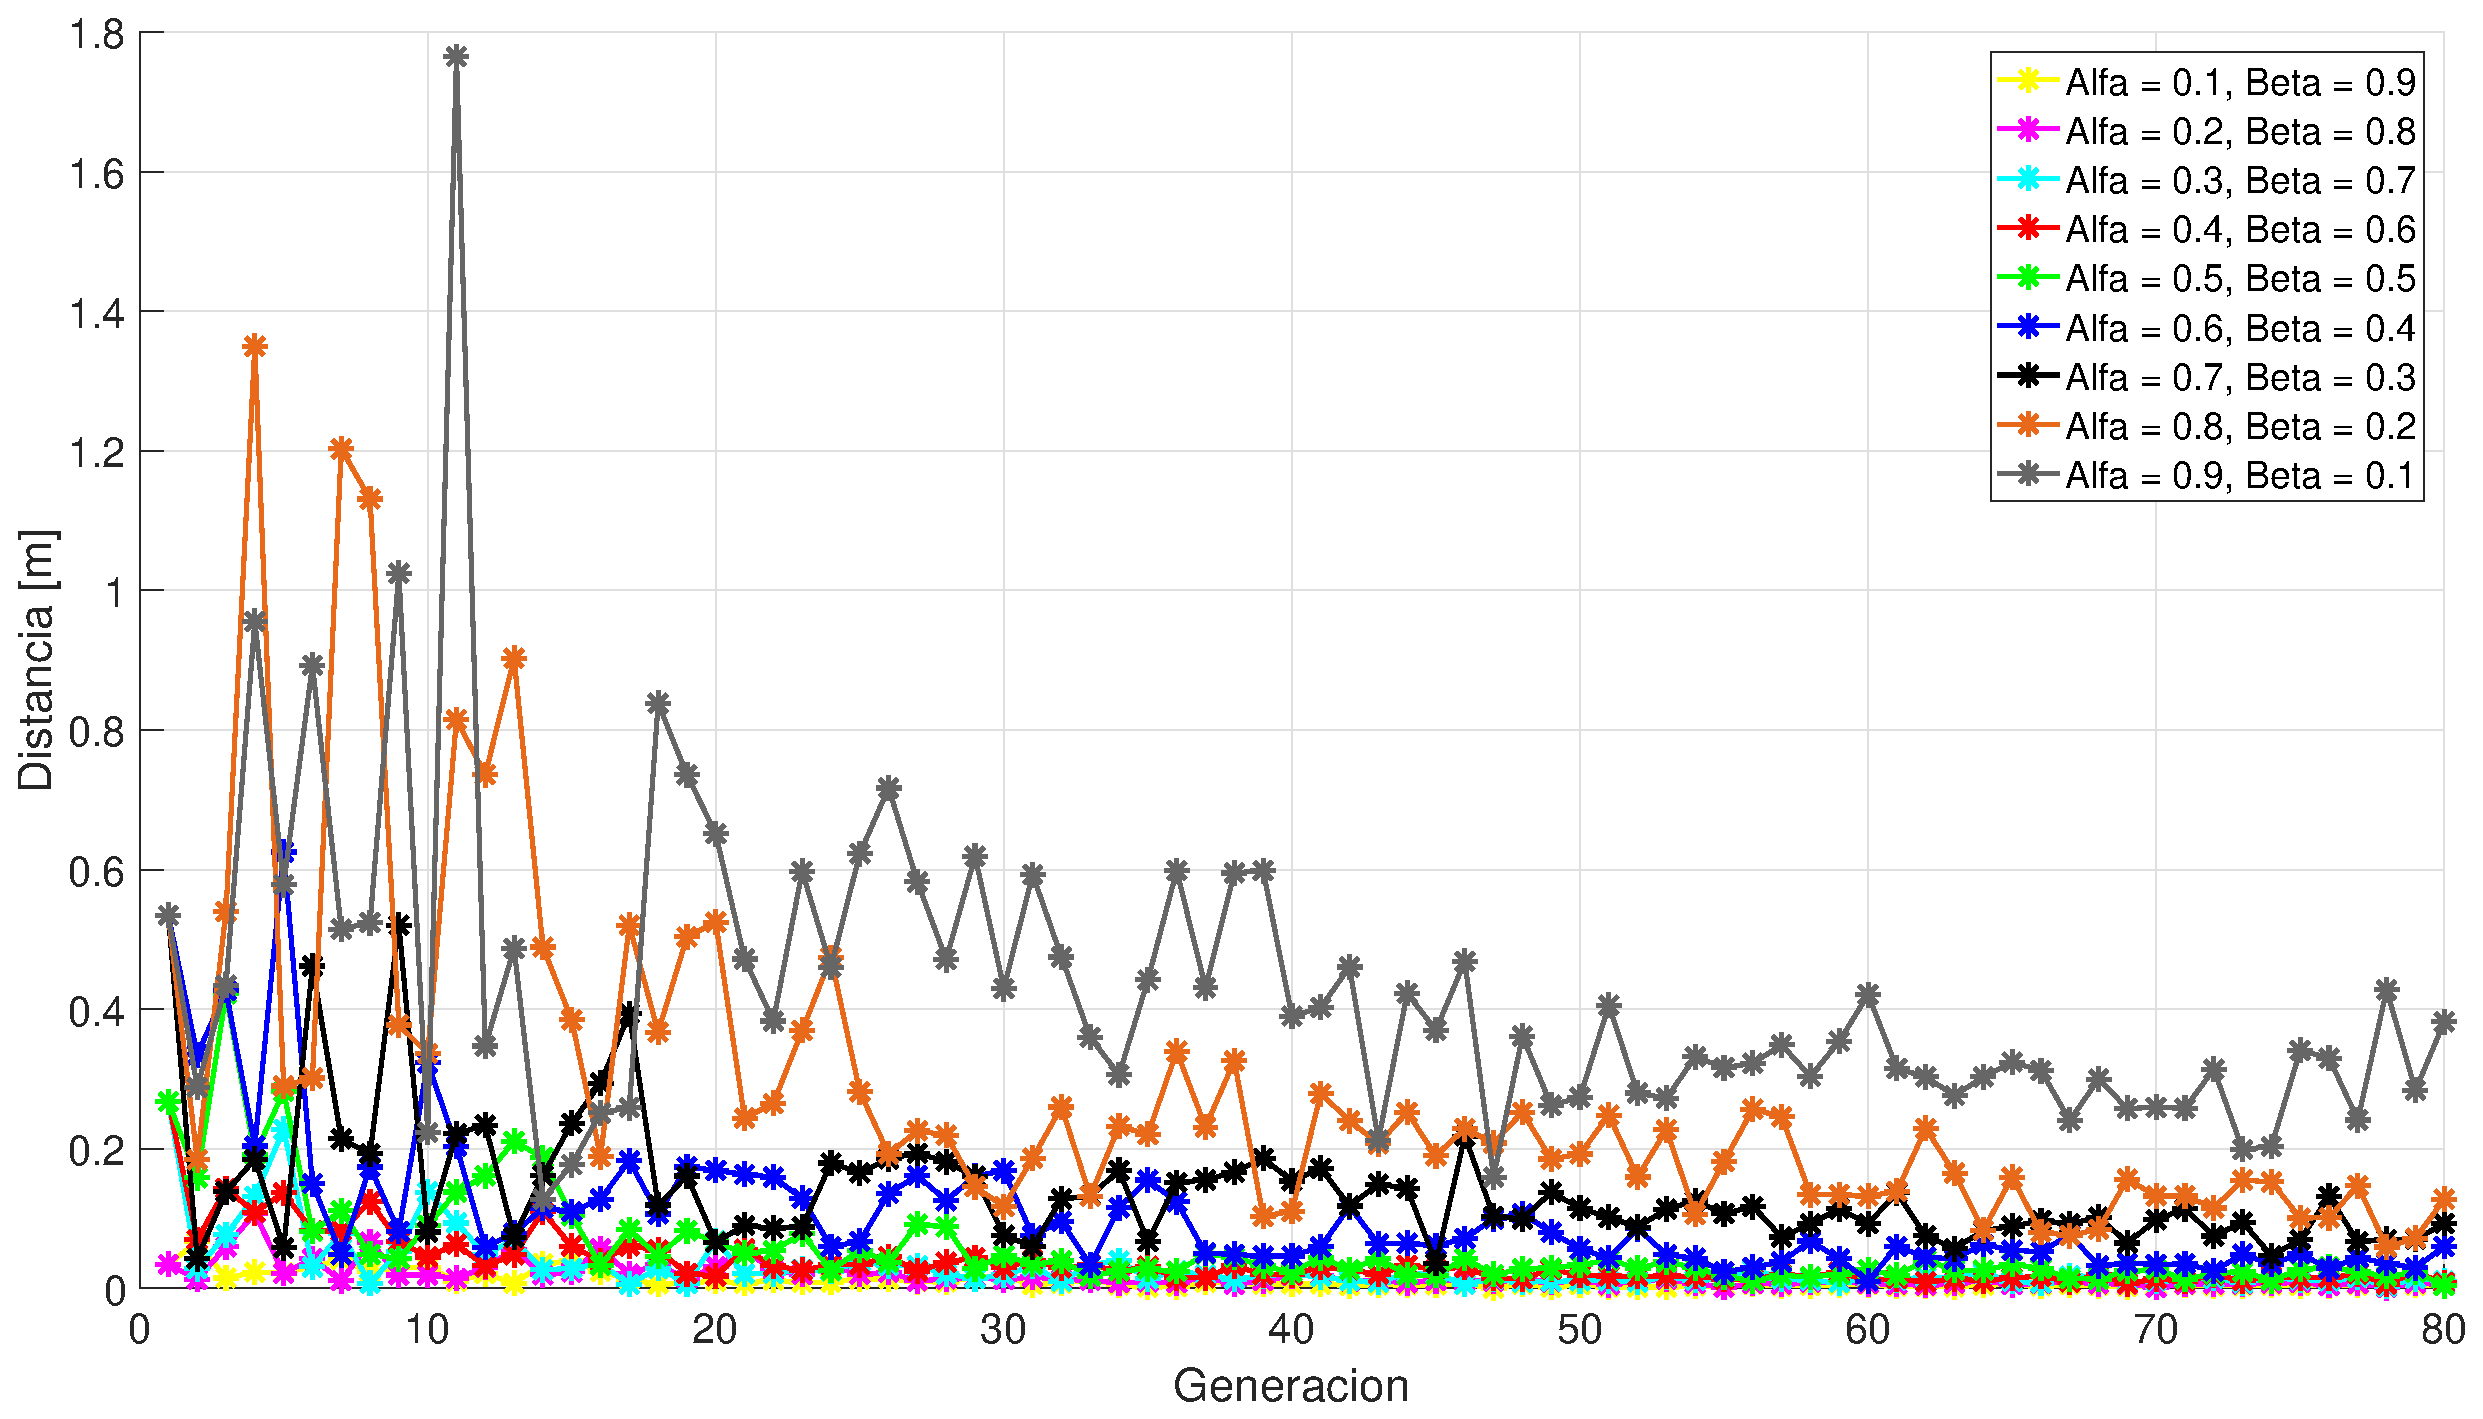
\includegraphics[width=7cm,height=3.5cm]{imag/VariacionAlfas/Evoluciondelerrordeposicionparaelmejorfitnessvarianhiperparametros.eps}}
\subfigure[Fitness promedio.]{\label{this2}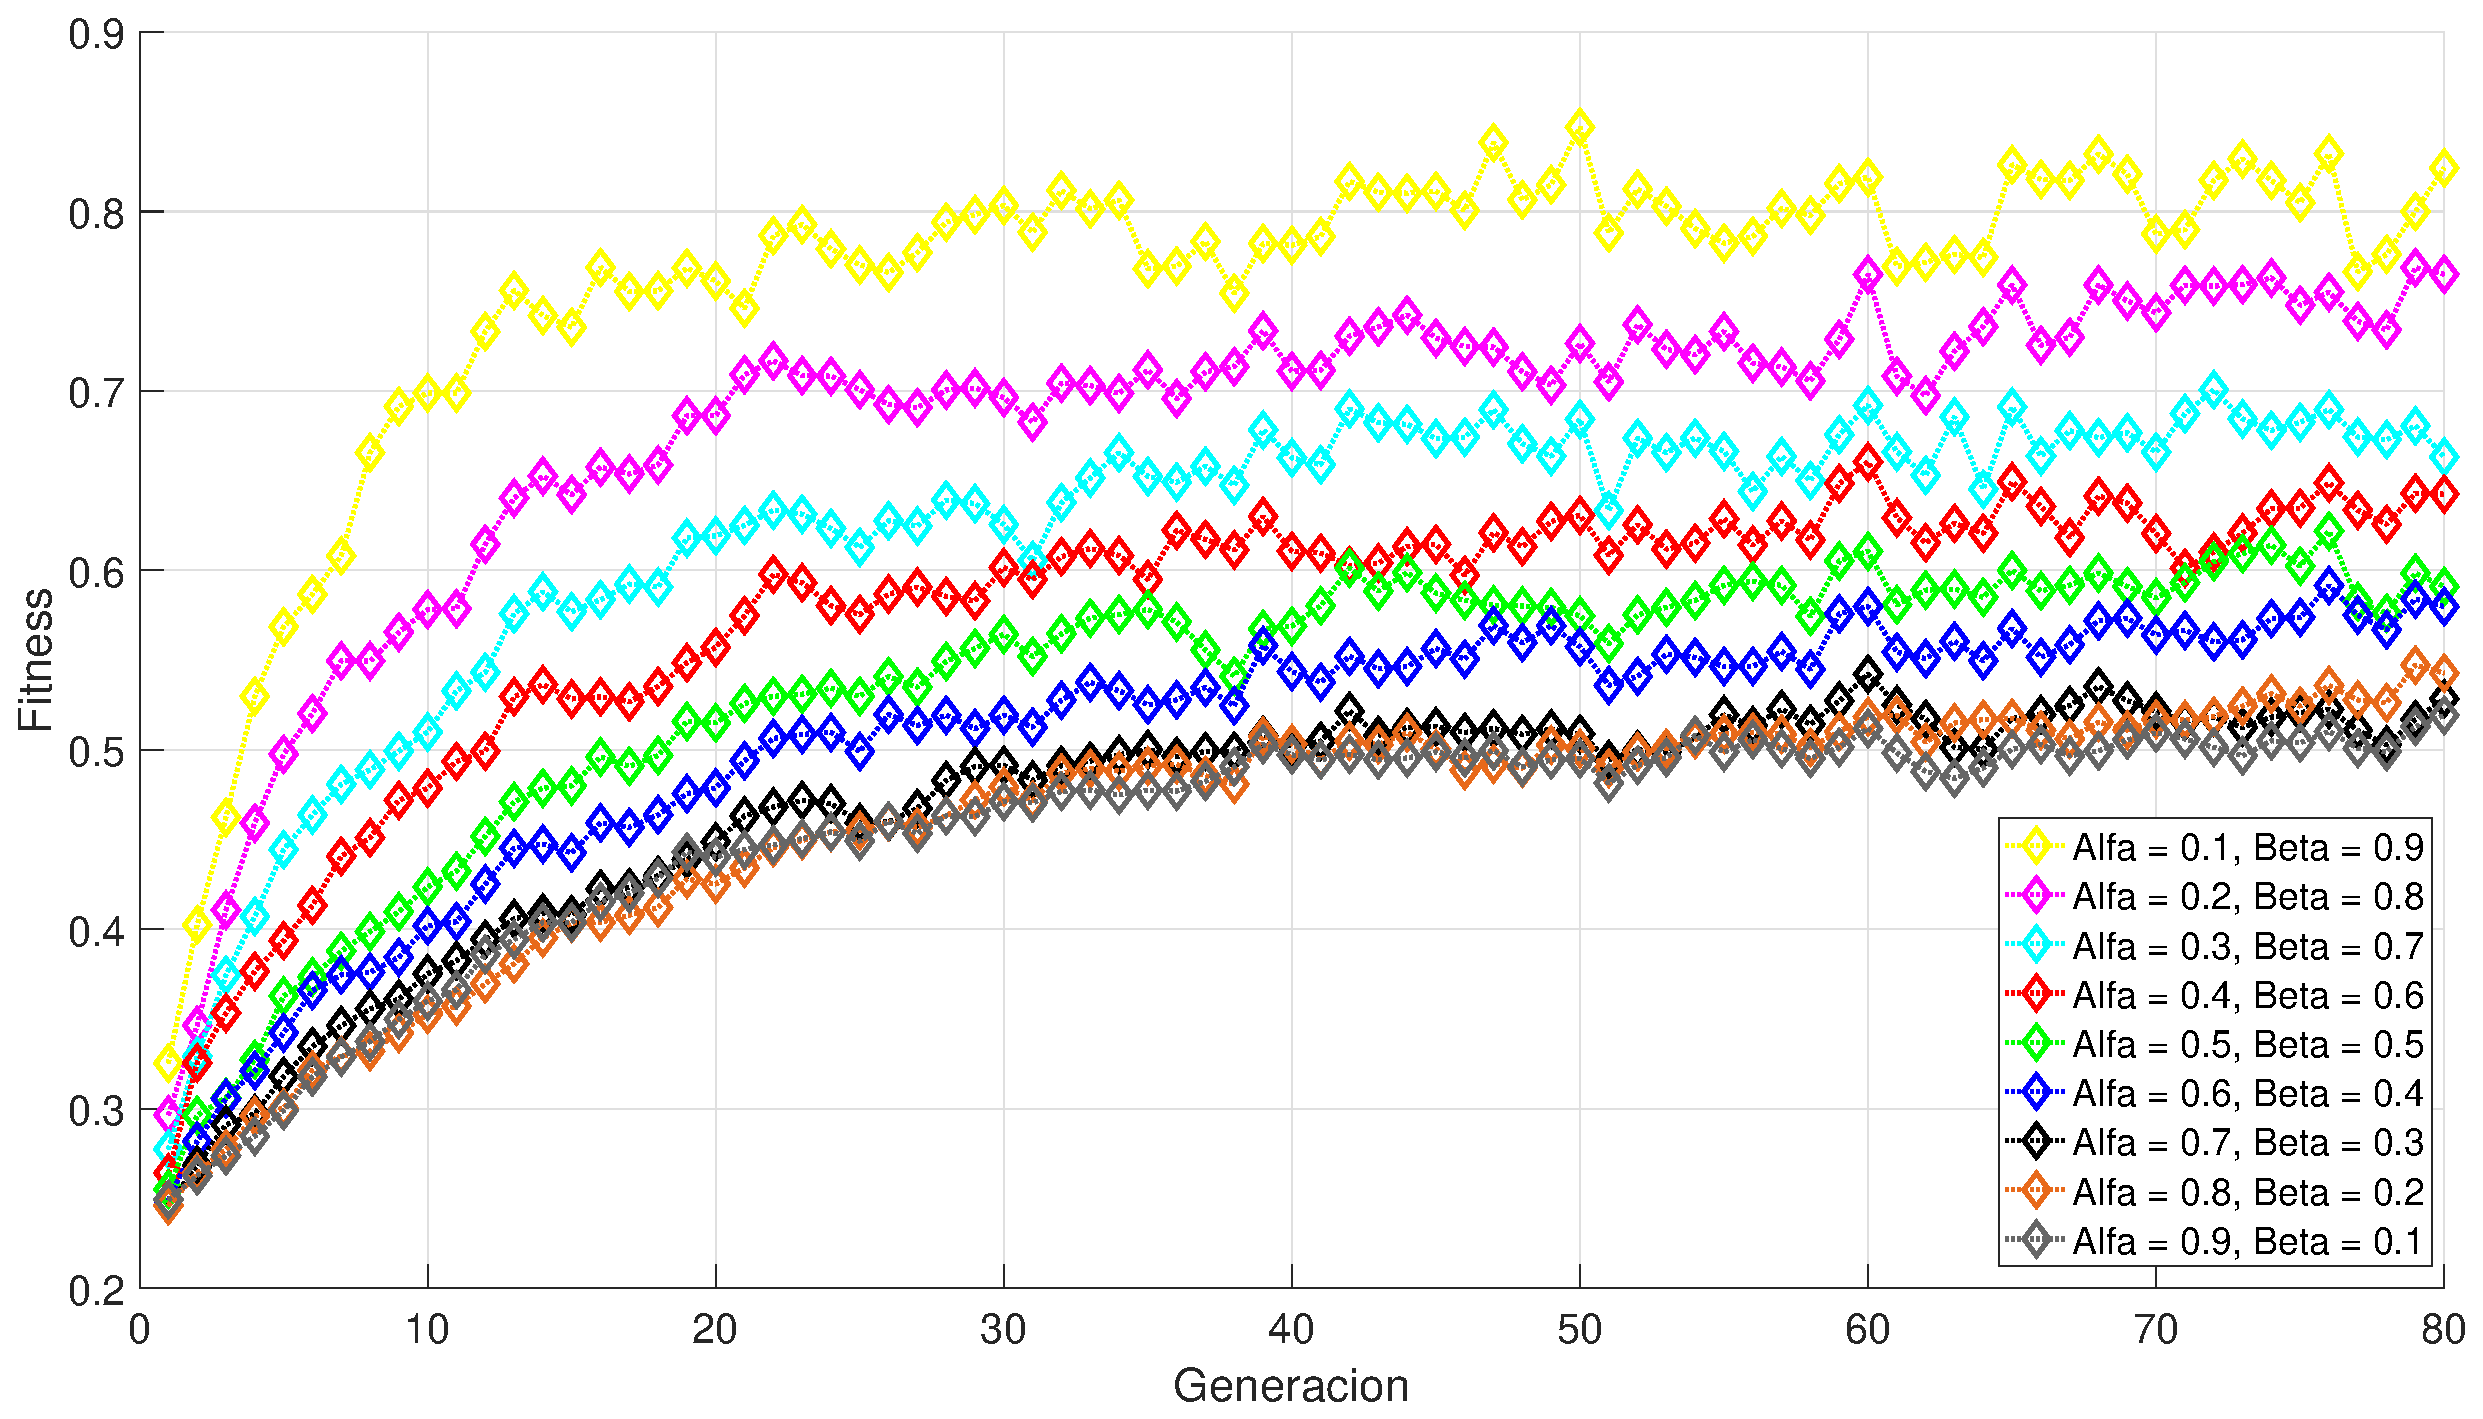
\includegraphics[width=7cm,height=3.5cm]{imag/VariacionAlfas/Fitnesspromedioparalasdistintasgeneracionesvarianhiperparametro.eps}}
\subfigure[Mejor fitness.]{\label{this3}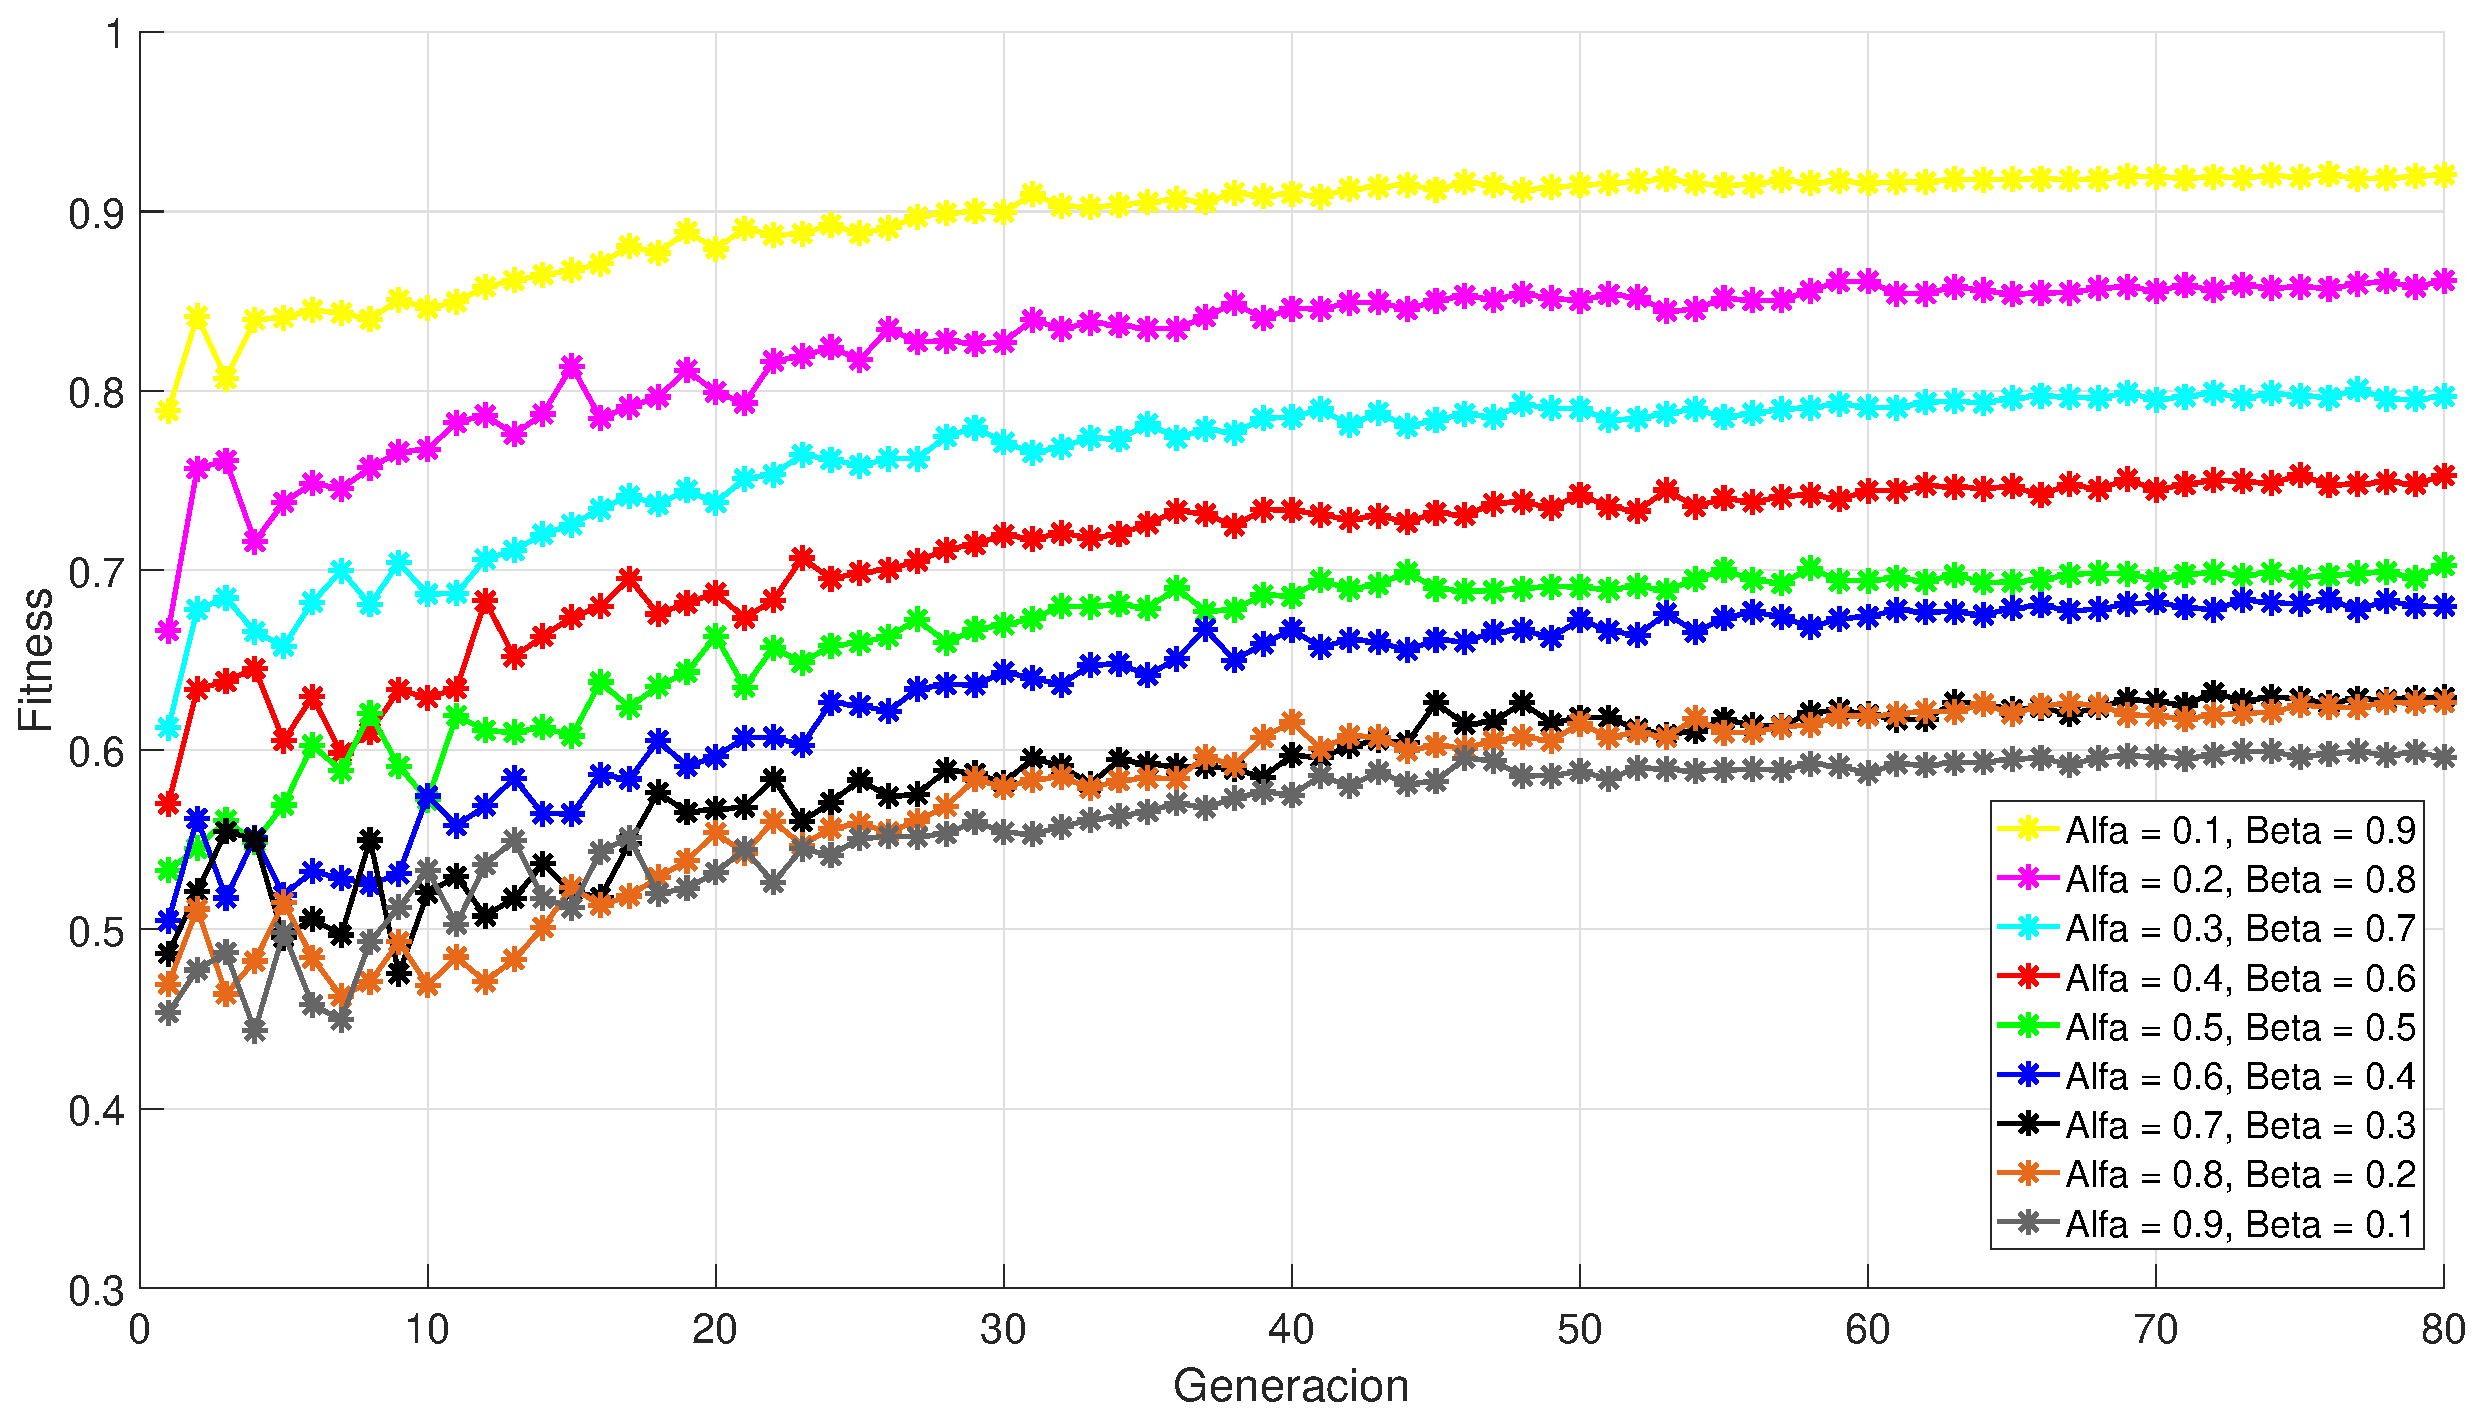
\includegraphics[width=14cm,height=3.5cm]{imag/VariacionAlfas/Evoluciondelmejorfitnessvarianhiperparametro.eps}}
\caption{Variación de los hiperparametros por generación.}
\label{muchas}
\end{figure}

No obstante y si se comparan estos resultados con la trayectoria que cada uno de estos casos tiene, obtenido mediante el método DH, y que se observa en la figura \ref{Primresultados} se tiene que las combinatorias de  $\alpha$ y $\beta$ que en la figura \ref{muchas} obtuvieron los mejores resultados así como los que entregaron los peores, son los que muestran trayectorias mas erráticas.

Para evitar estos casos extremos es que se decidió que los hiperparametros $\alpha$ y $\beta$ fuesen de 0.5 cada uno, esperando que de esta manera los resultados mostrasen un comportamiento mas homogéneo.


\begin{figure}
\centering
\subfigure[$\alpha$: 0.1 y $\beta$: 0.9]{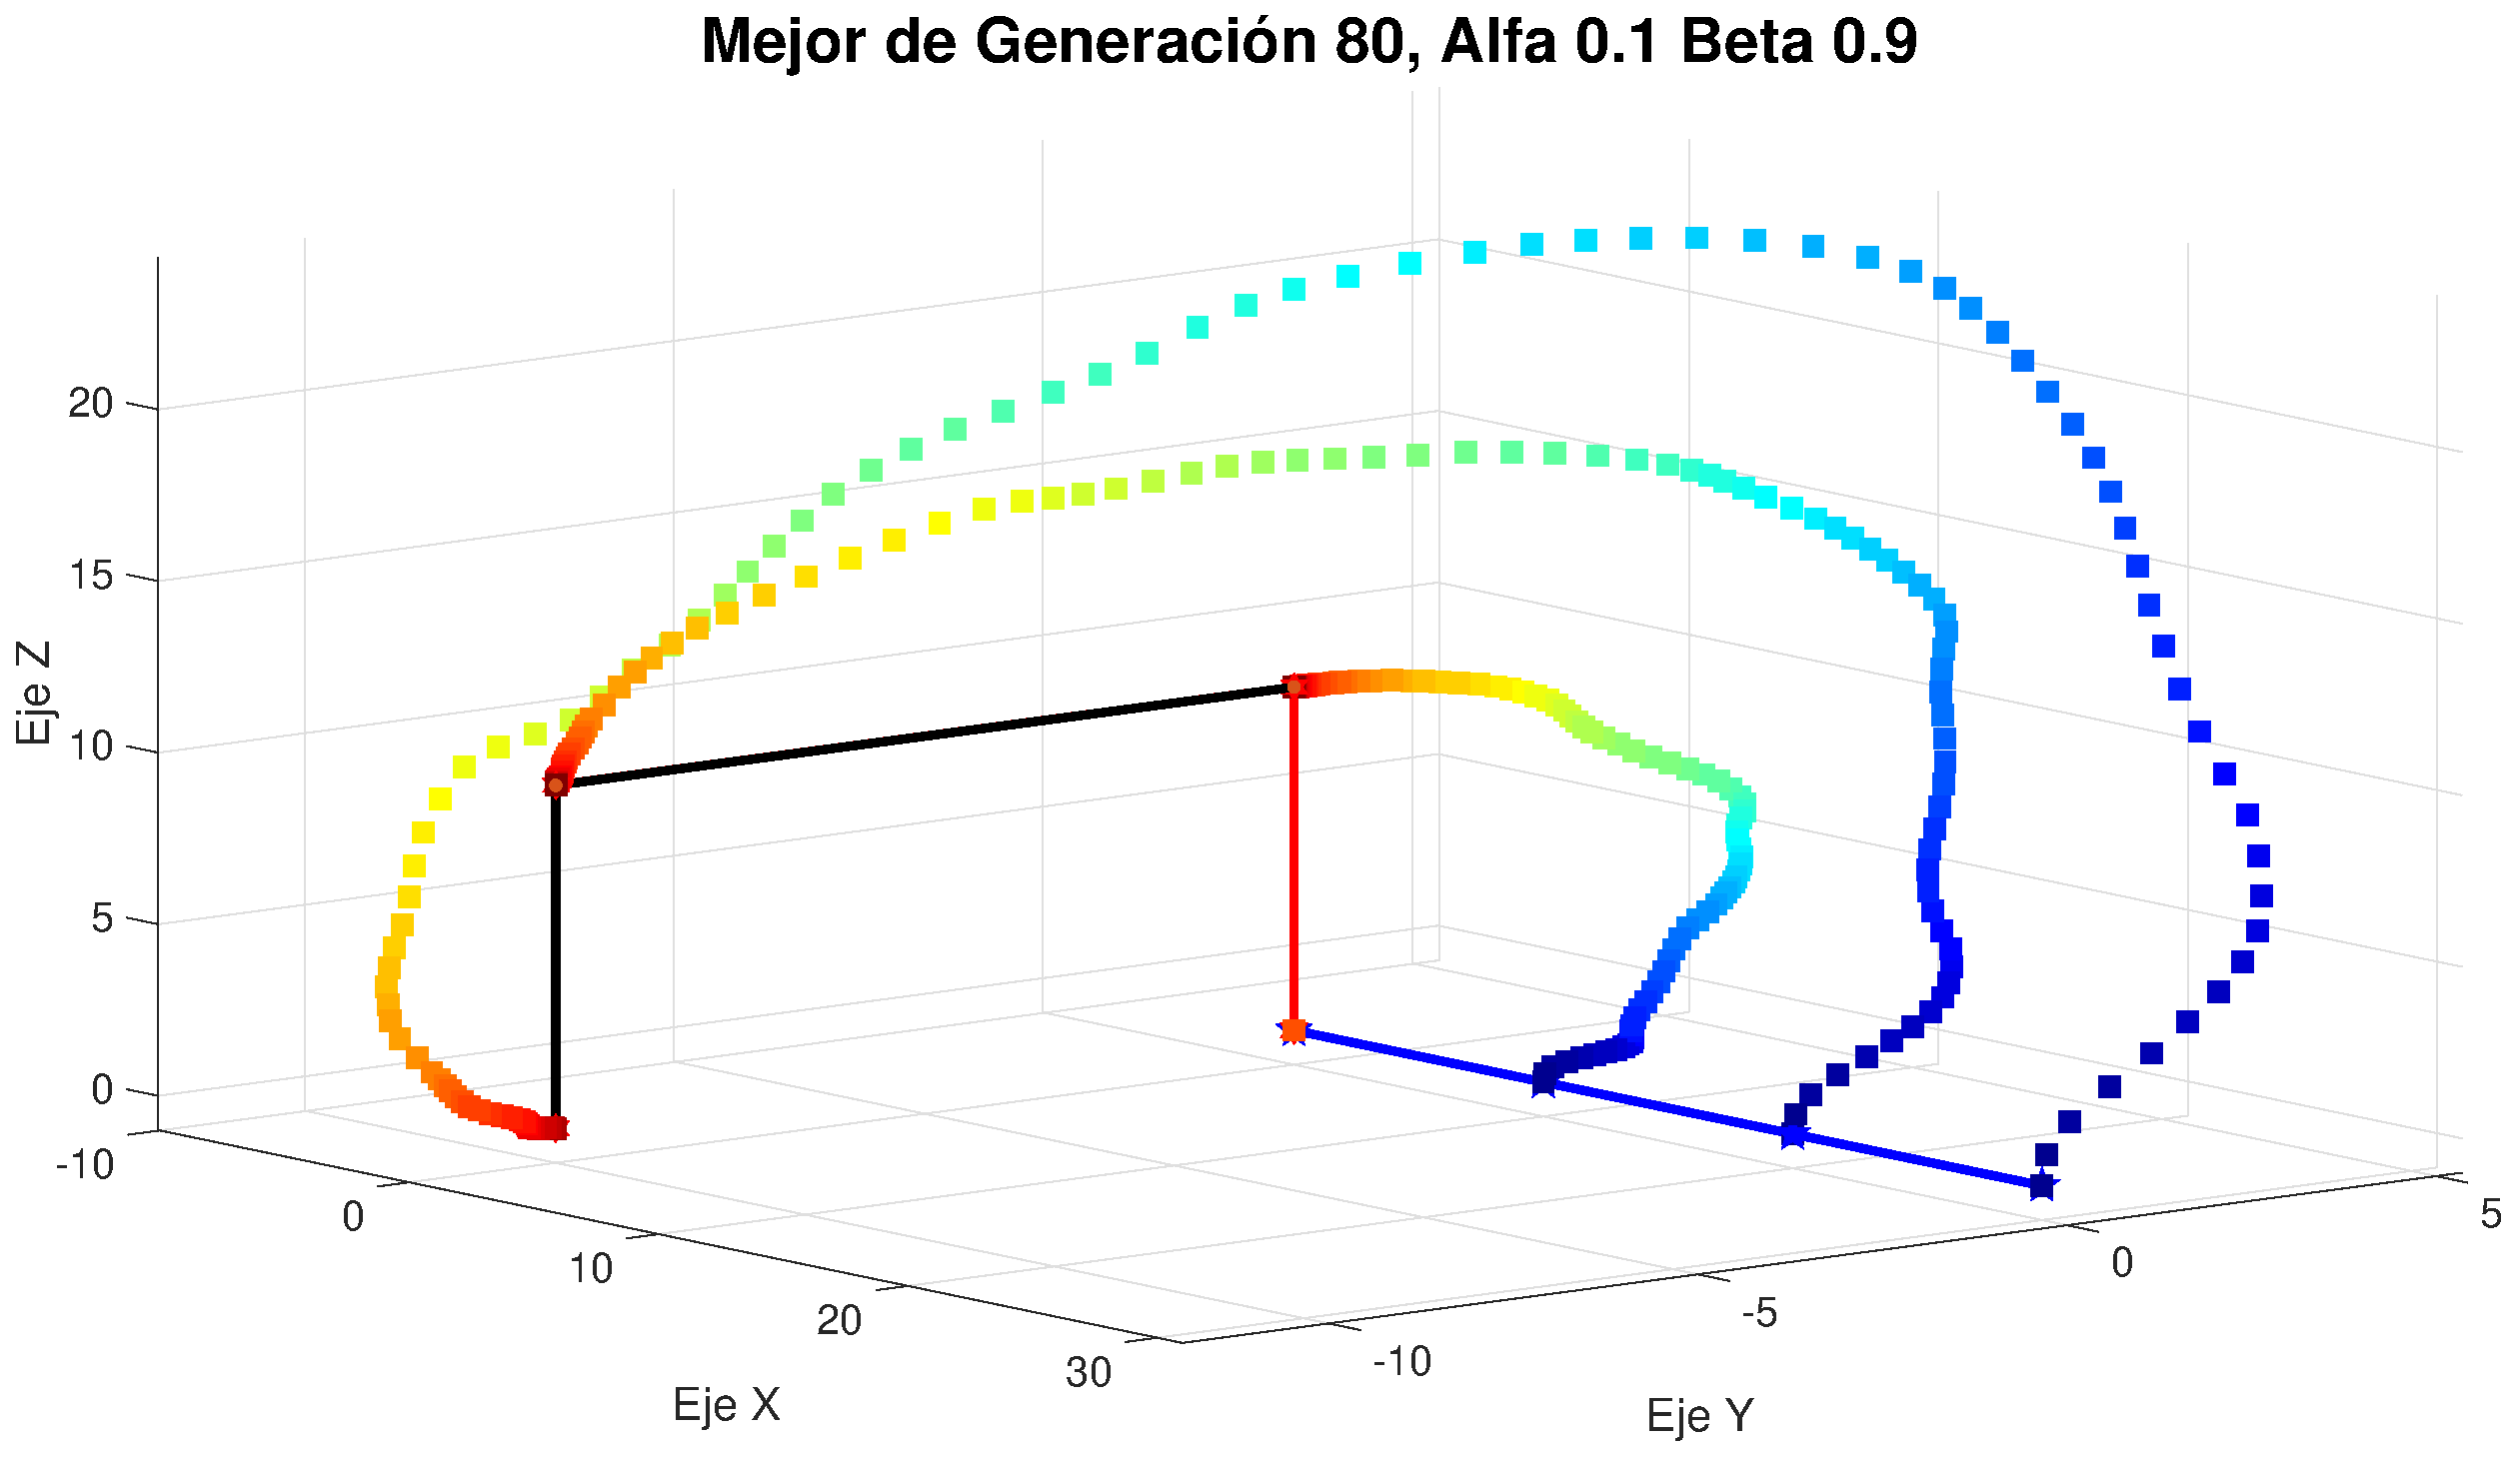
\includegraphics[width=4cm,height=2cm]{imag/VariacionAlfas/Alfa01Beta09.eps}}
\subfigure[$\alpha$: 0.2 y $\beta$: 0.8]{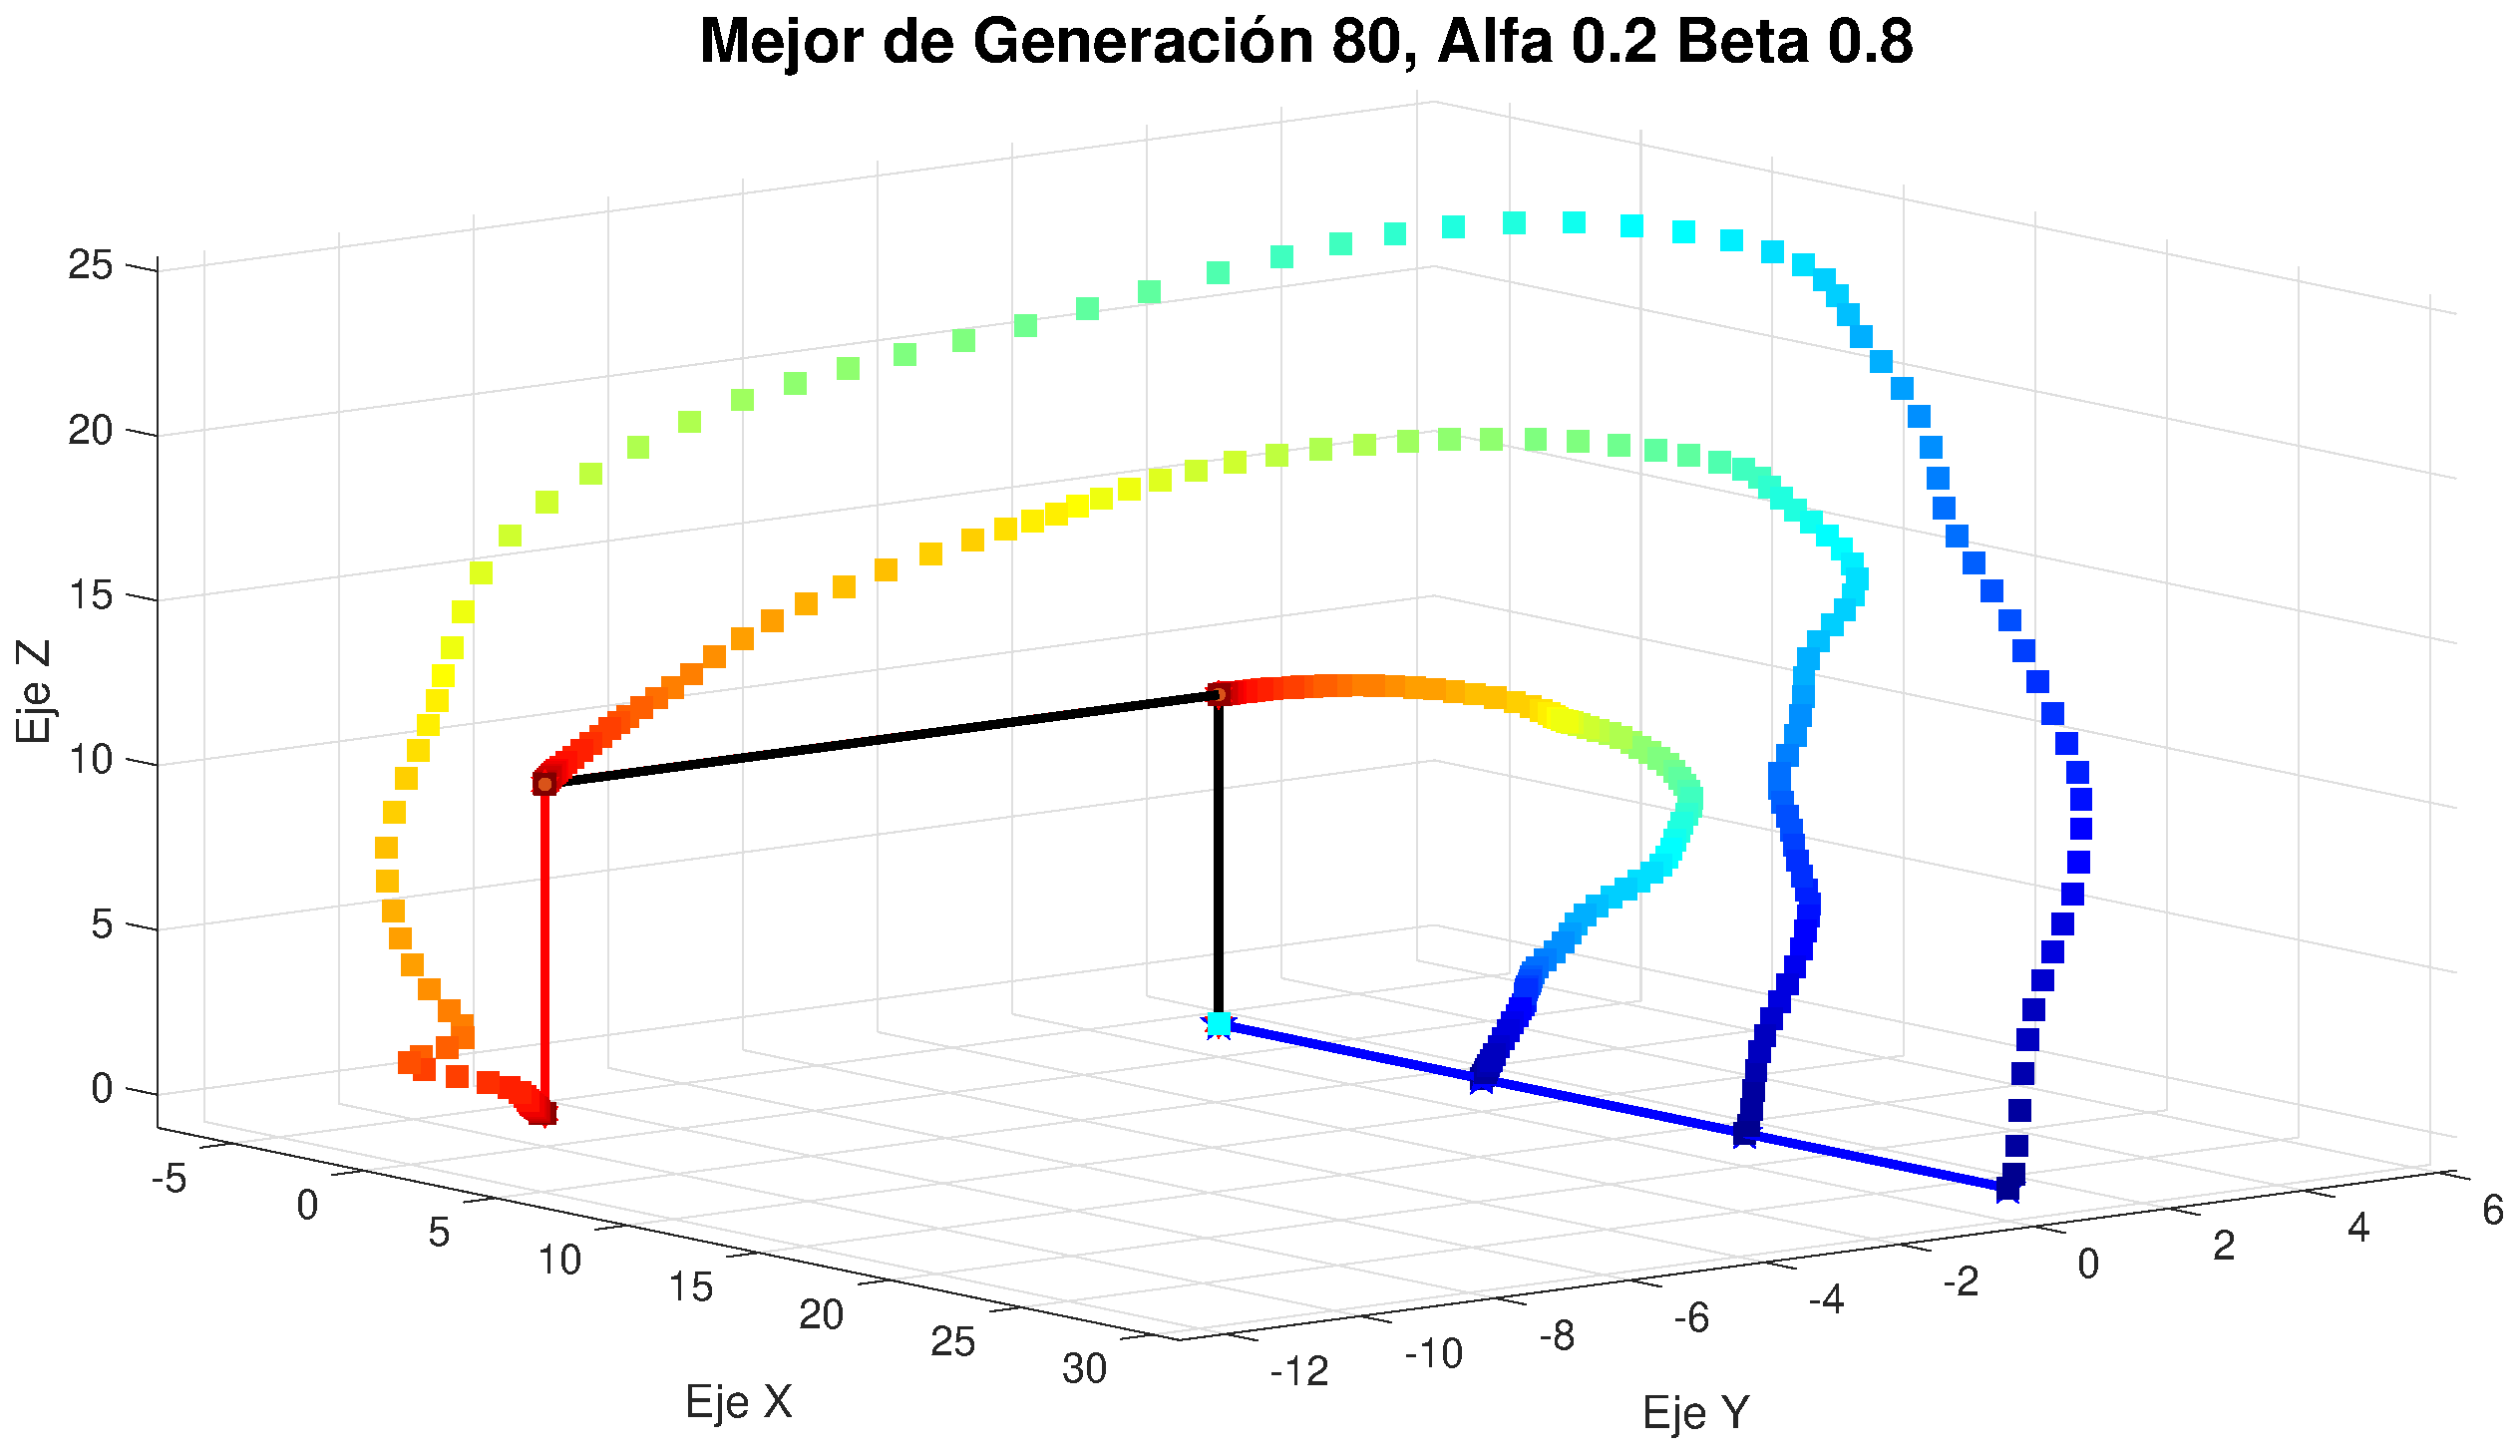
\includegraphics[width=4cm,height=2cm]{imag/VariacionAlfas/Alfa02Beta08.eps}}
\subfigure[$\alpha$: 0.3 y $\beta$: 0.7]{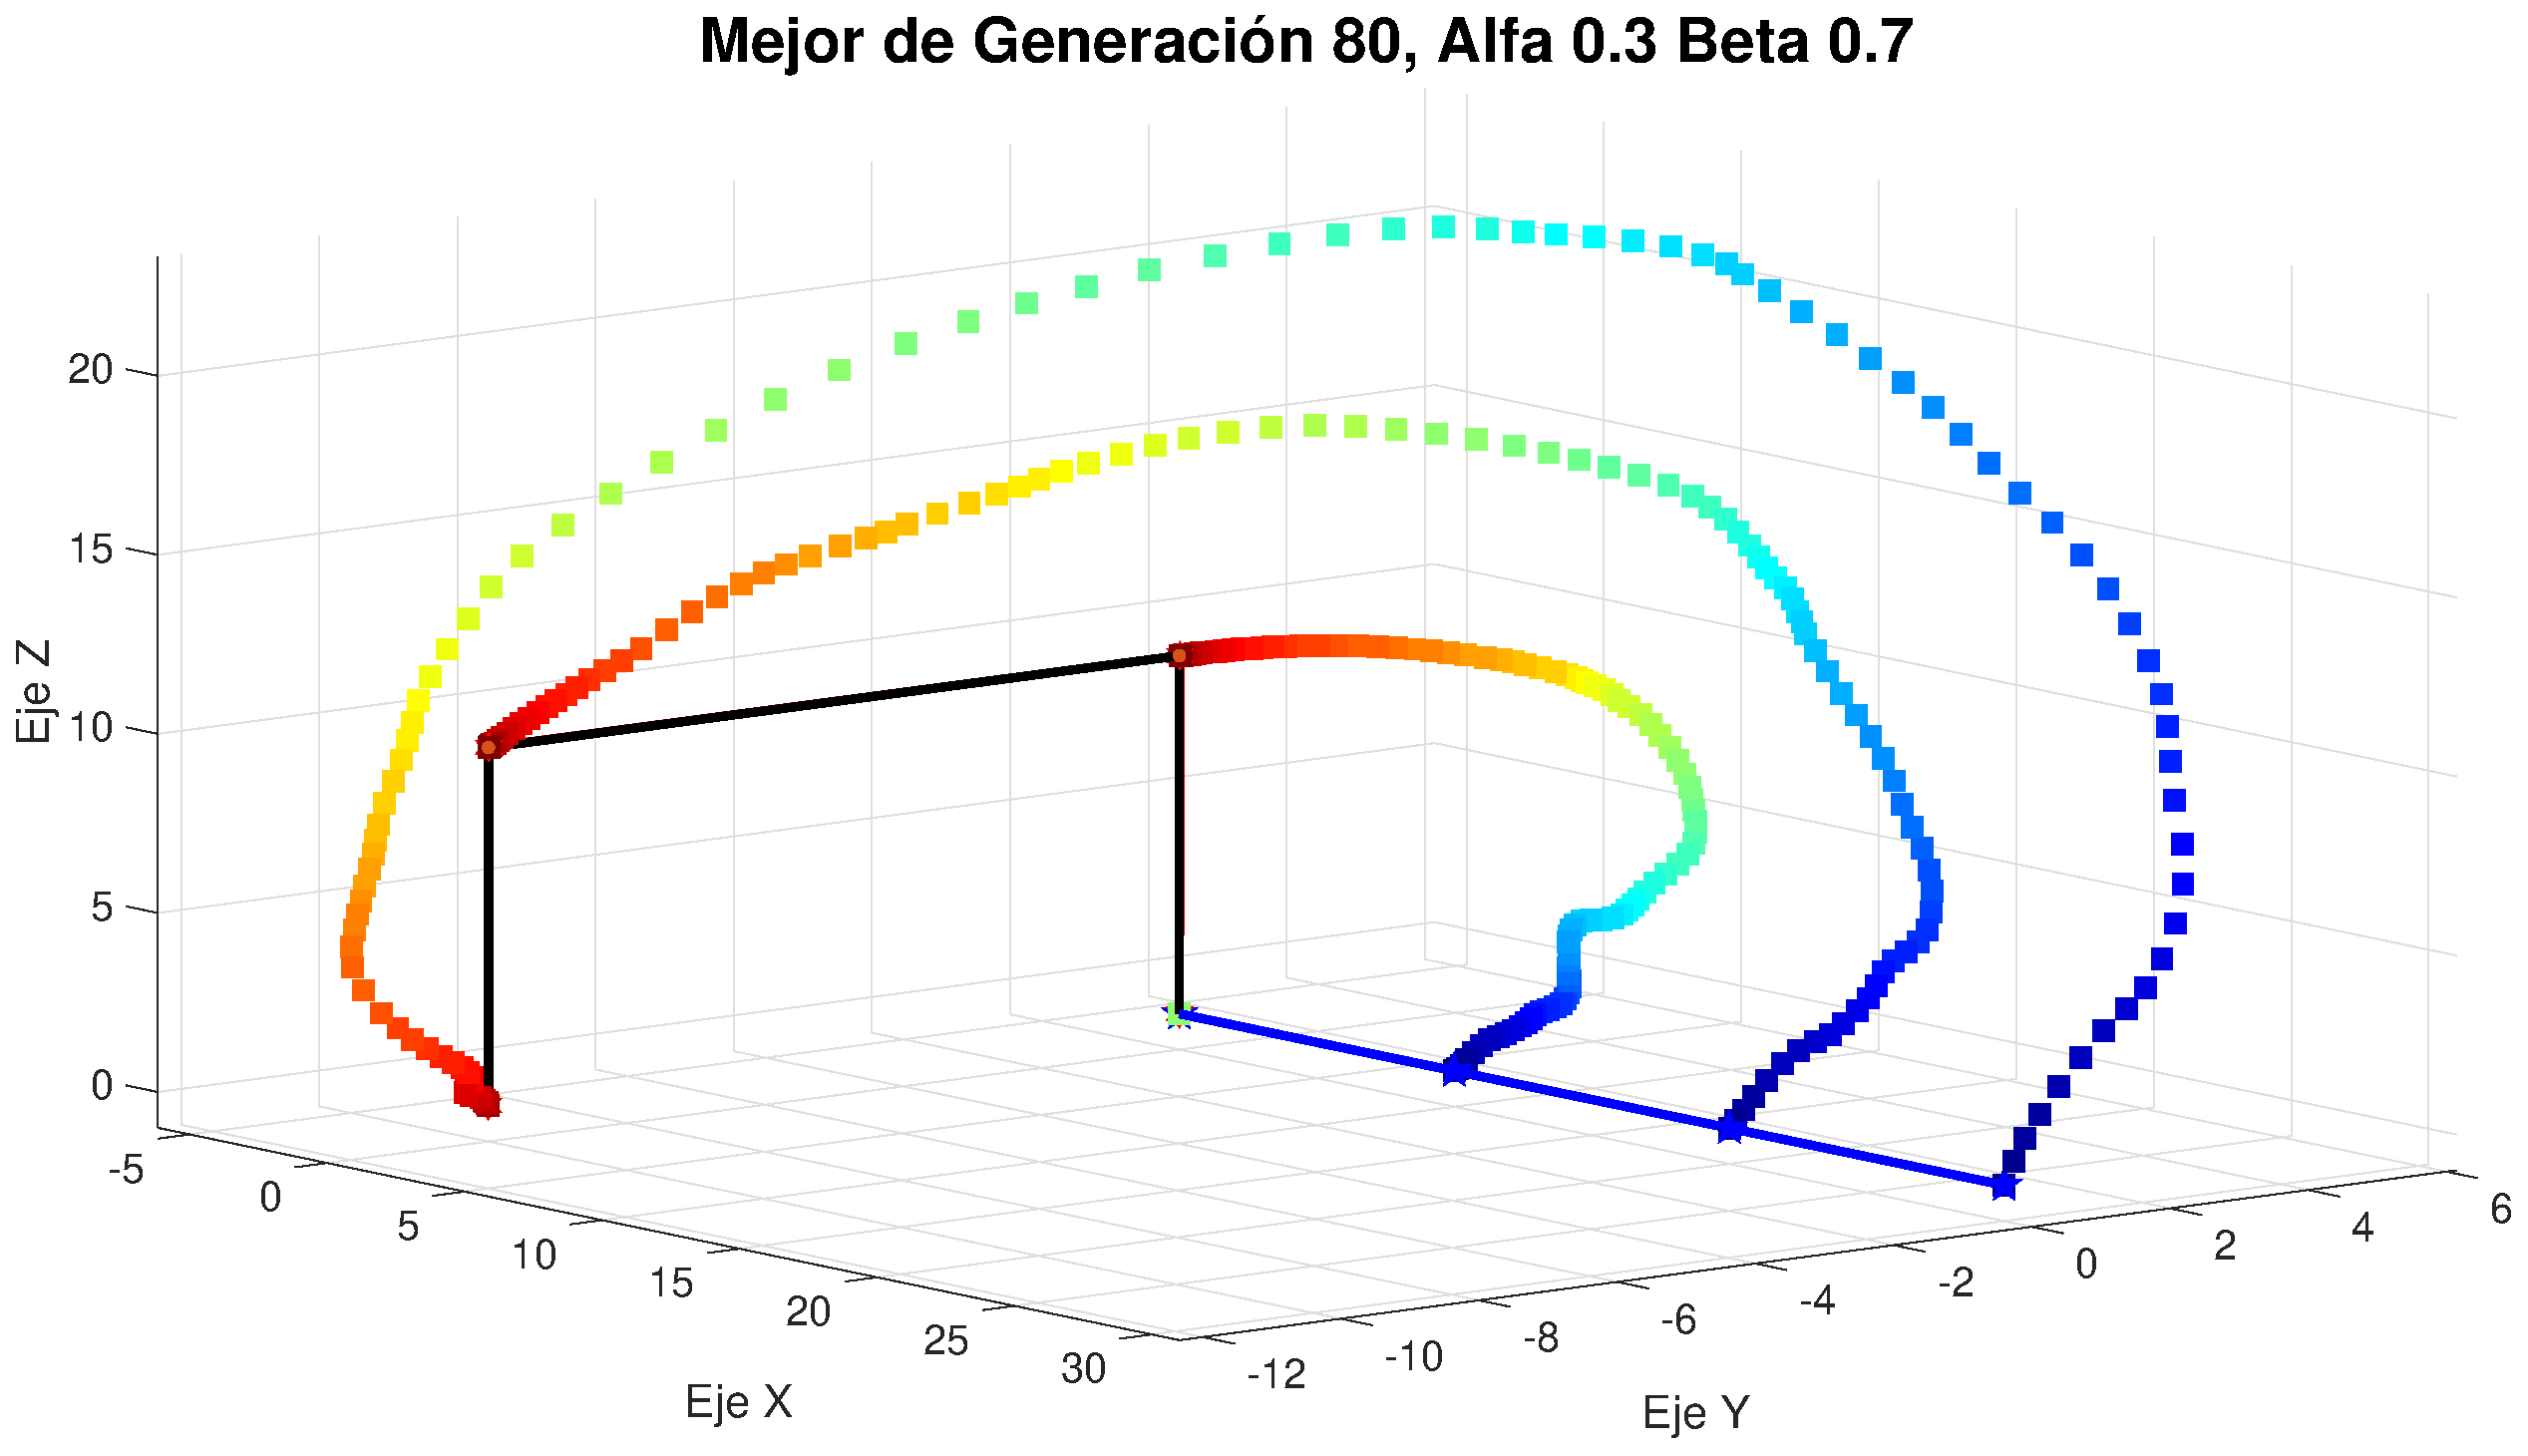
\includegraphics[width=4cm,height=2cm]{imag/VariacionAlfas/Alfa03Beta07.eps}}

\subfigure[$\alpha$: 0.4 y $\beta$: 0.6]{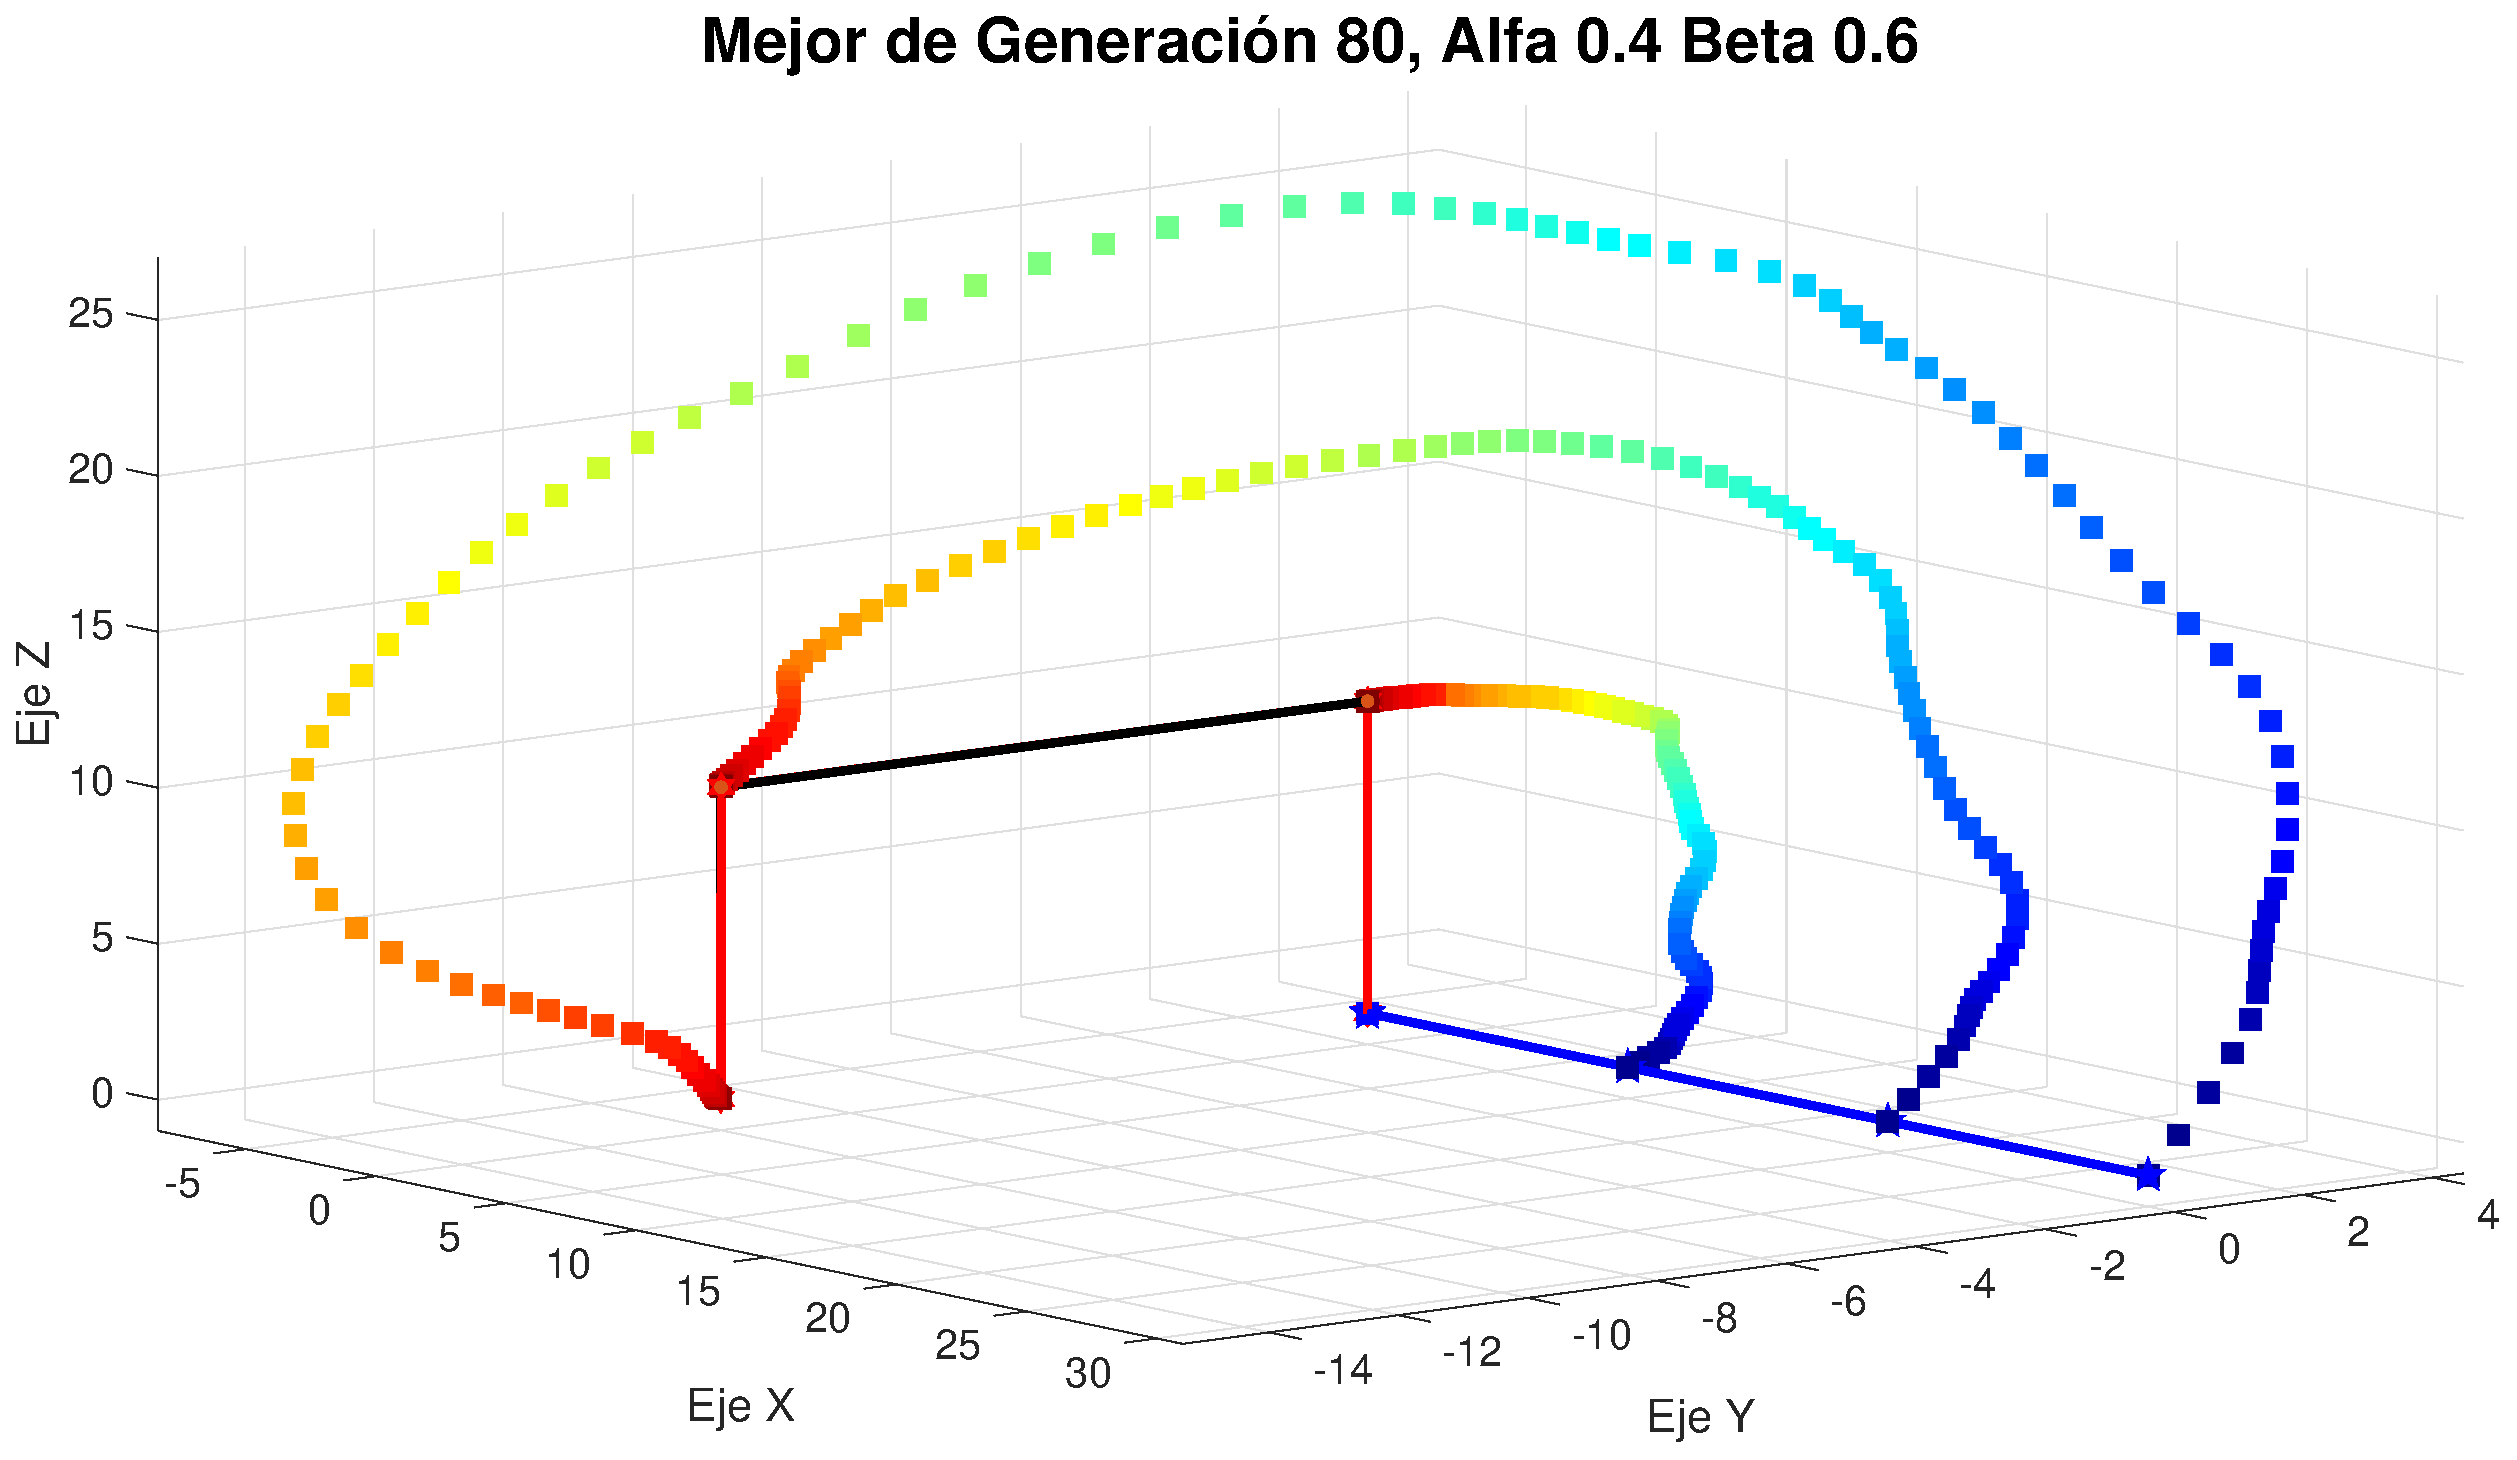
\includegraphics[width=4cm,height=2cm]{imag/VariacionAlfas/Alfa04Beta06.eps}}
\subfigure[$\alpha$: 0.5 y $\beta$: 0.5]{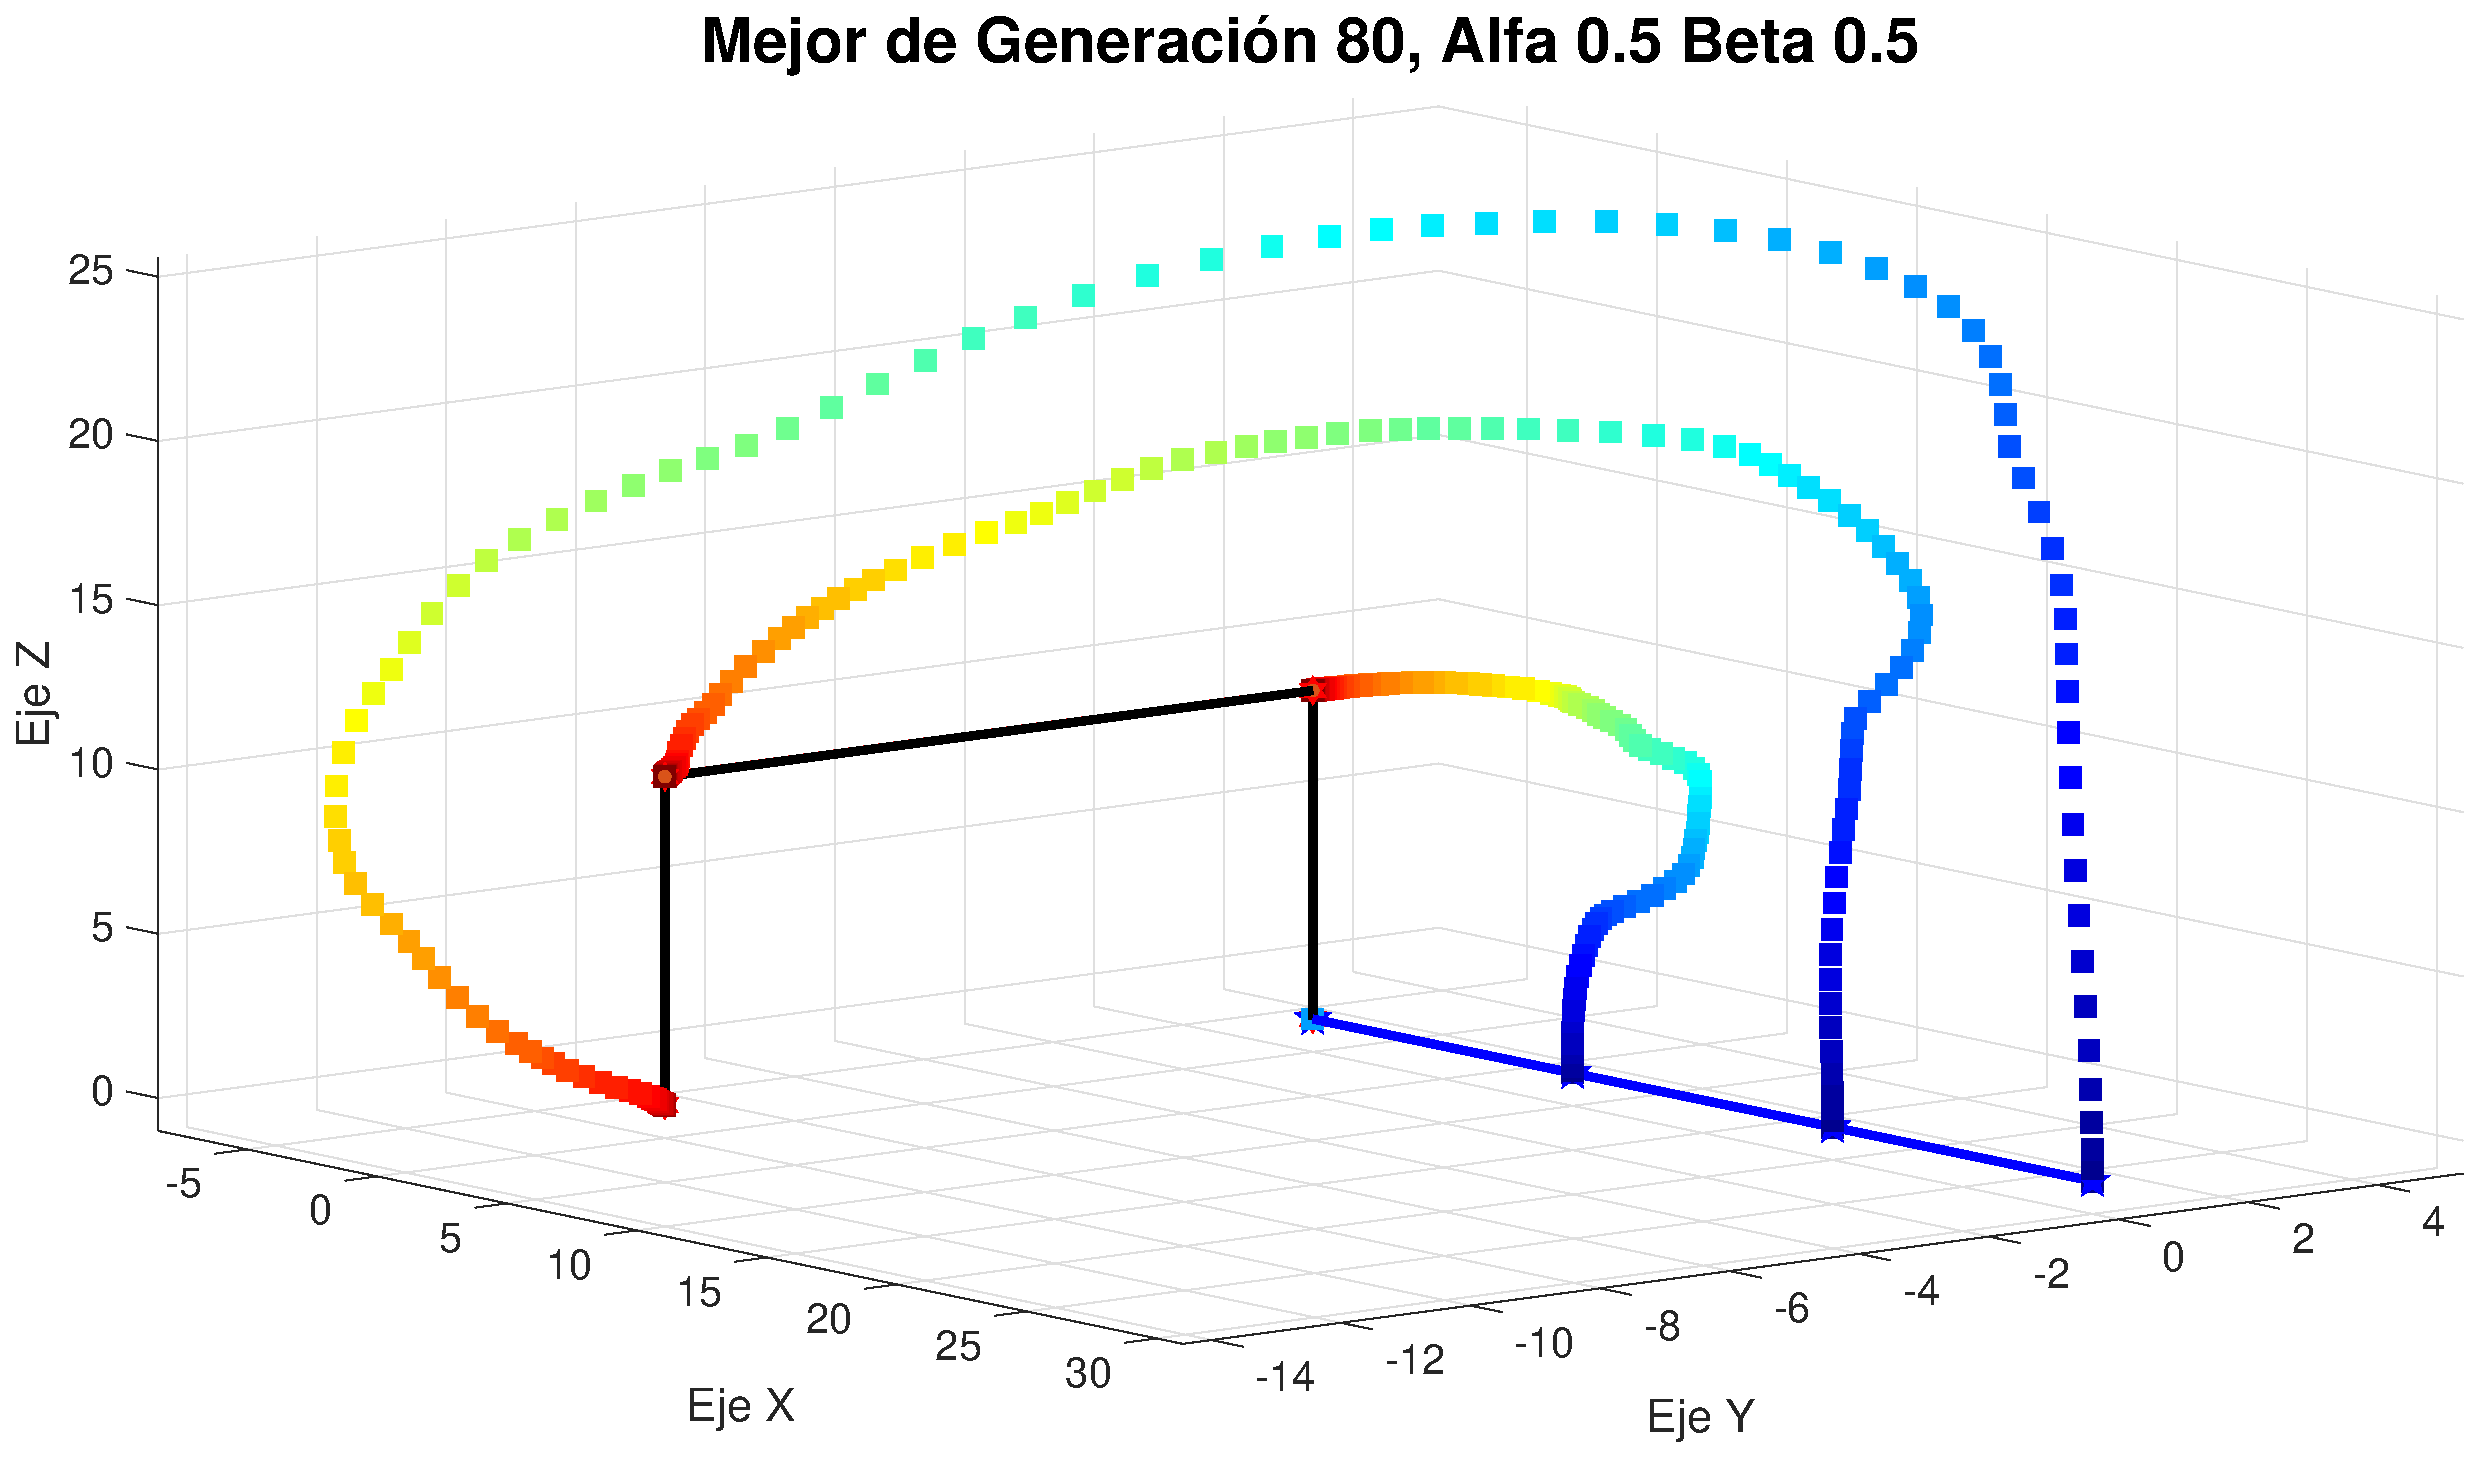
\includegraphics[width=4cm,height=2cm]{imag/VariacionAlfas/Alfa05Beta05.eps}}
\subfigure[$\alpha$: 0.6 y $\beta$ 0.4]{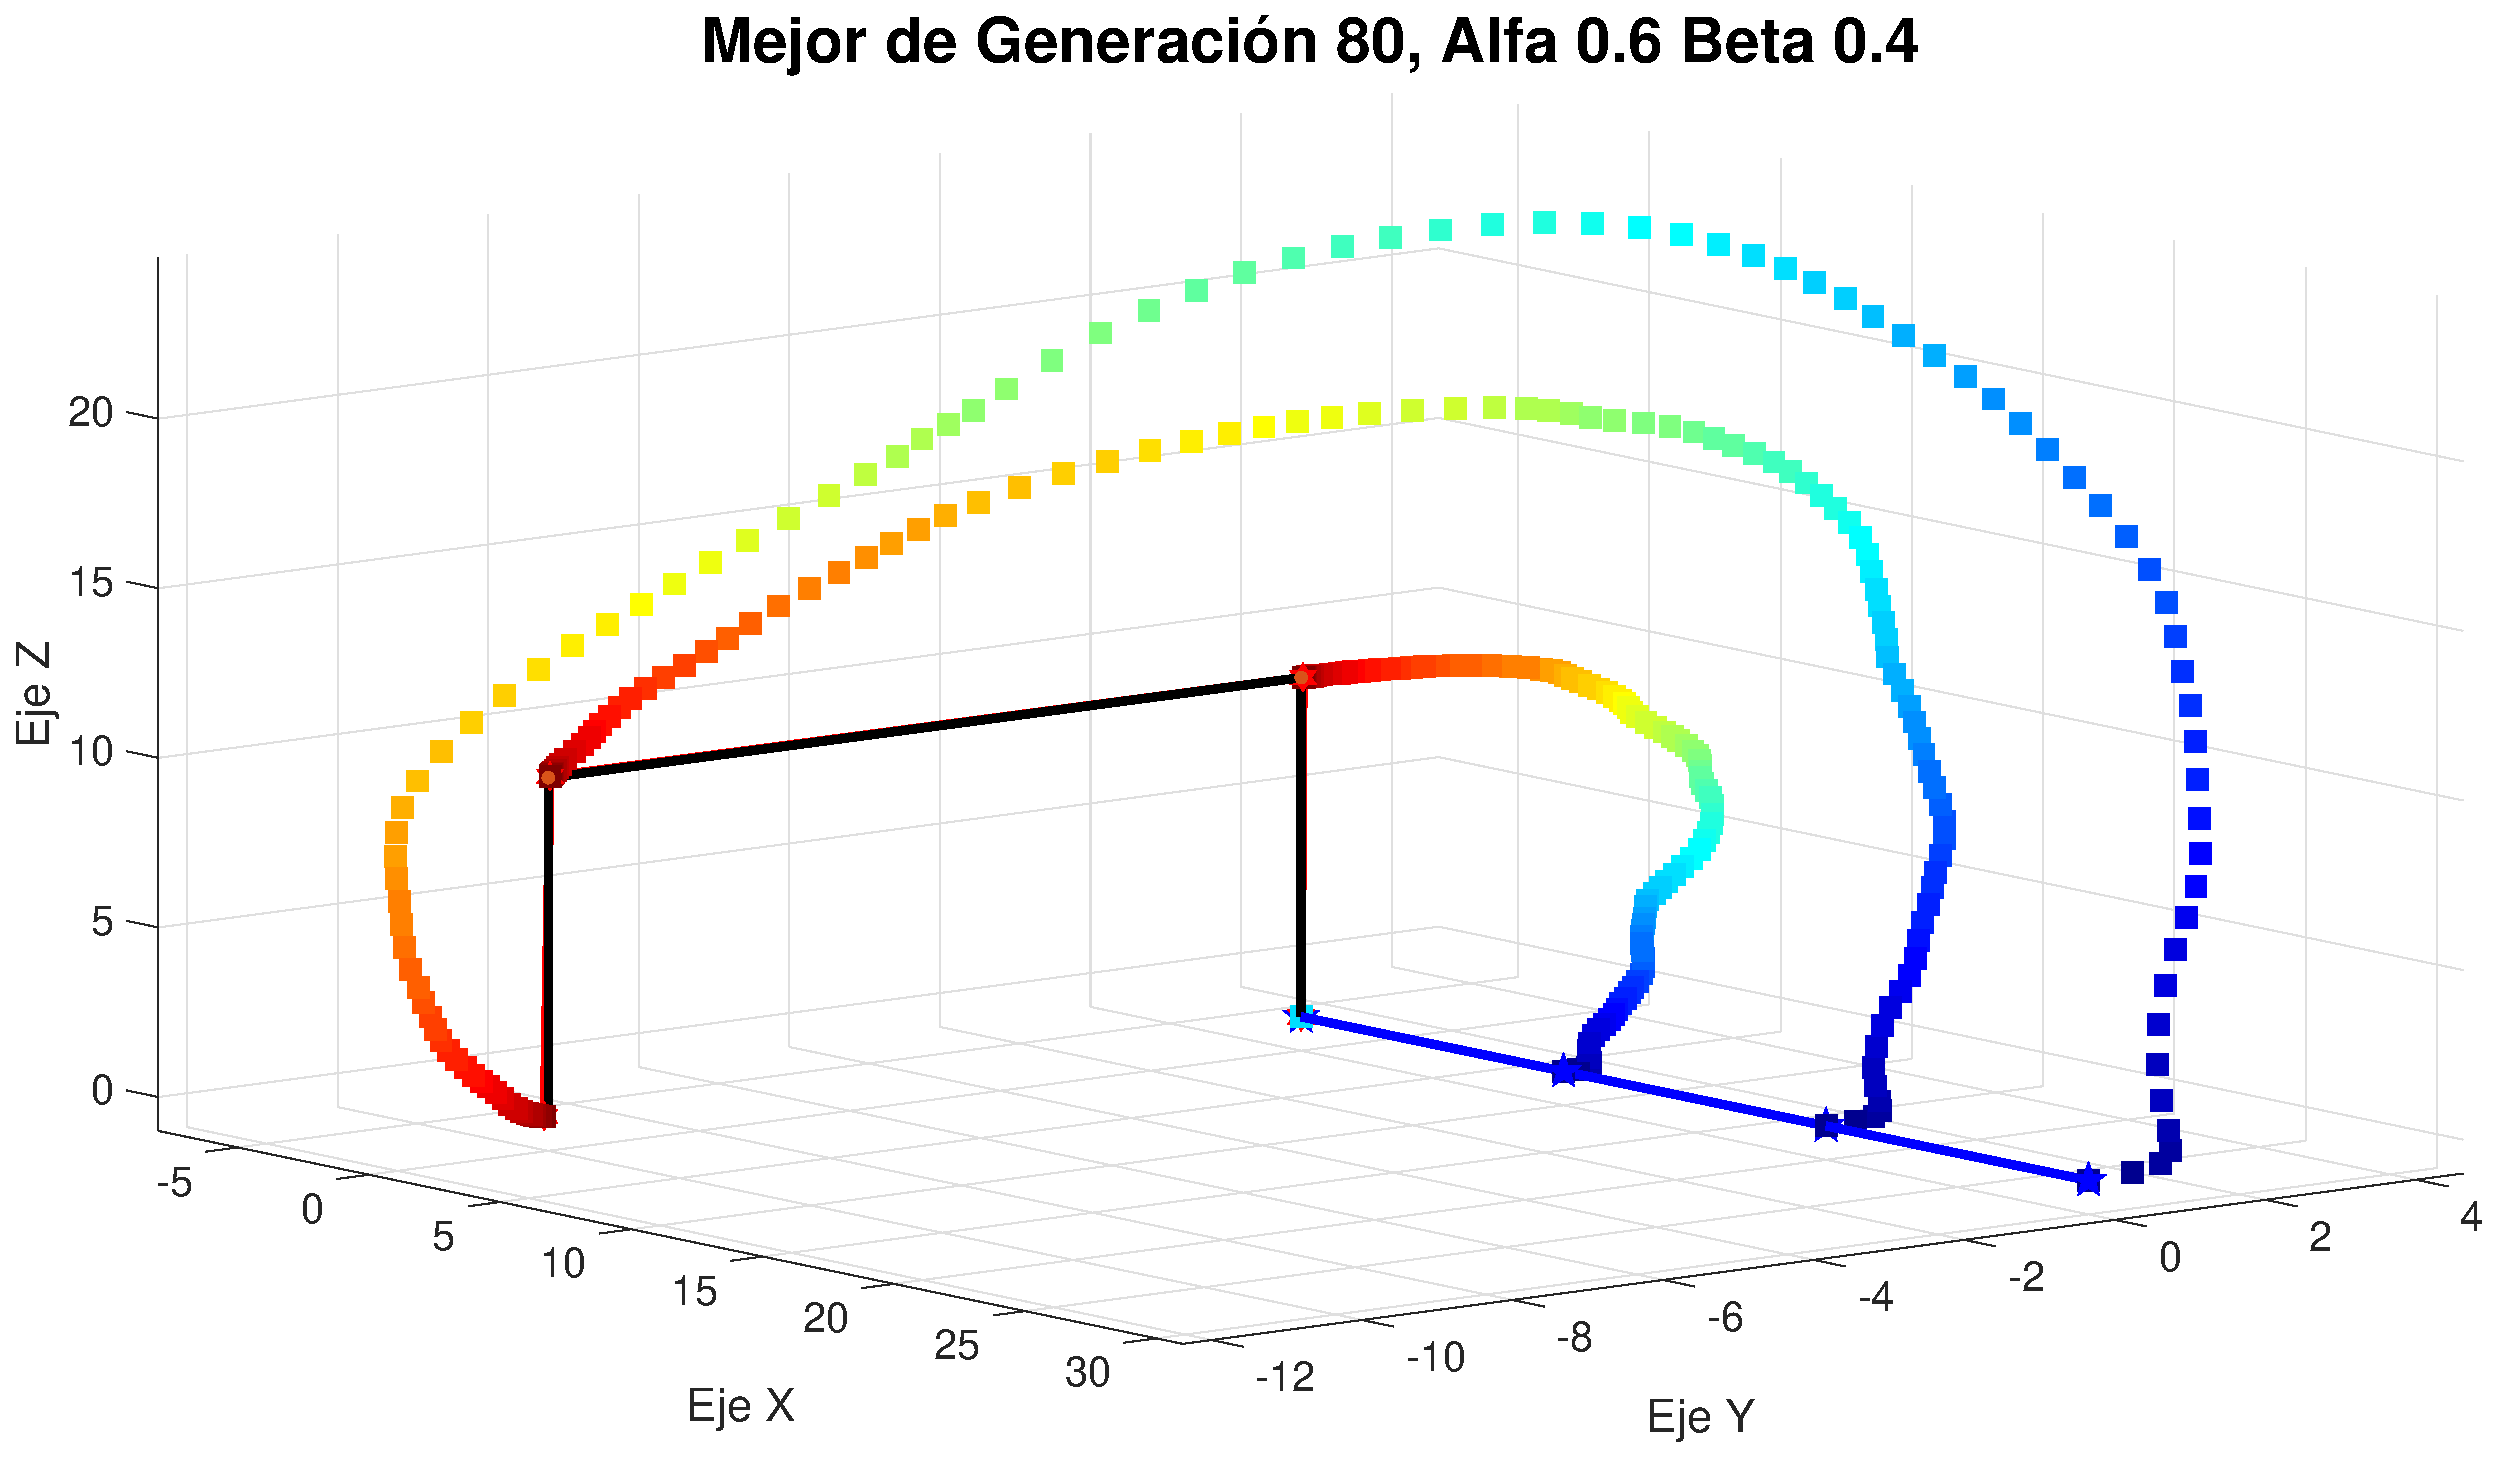
\includegraphics[width=4cm,height=2cm]{imag/VariacionAlfas/Alfa06Beta04.eps}}

\subfigure[$\alpha$: 0.7 y $\beta$: 0.3]{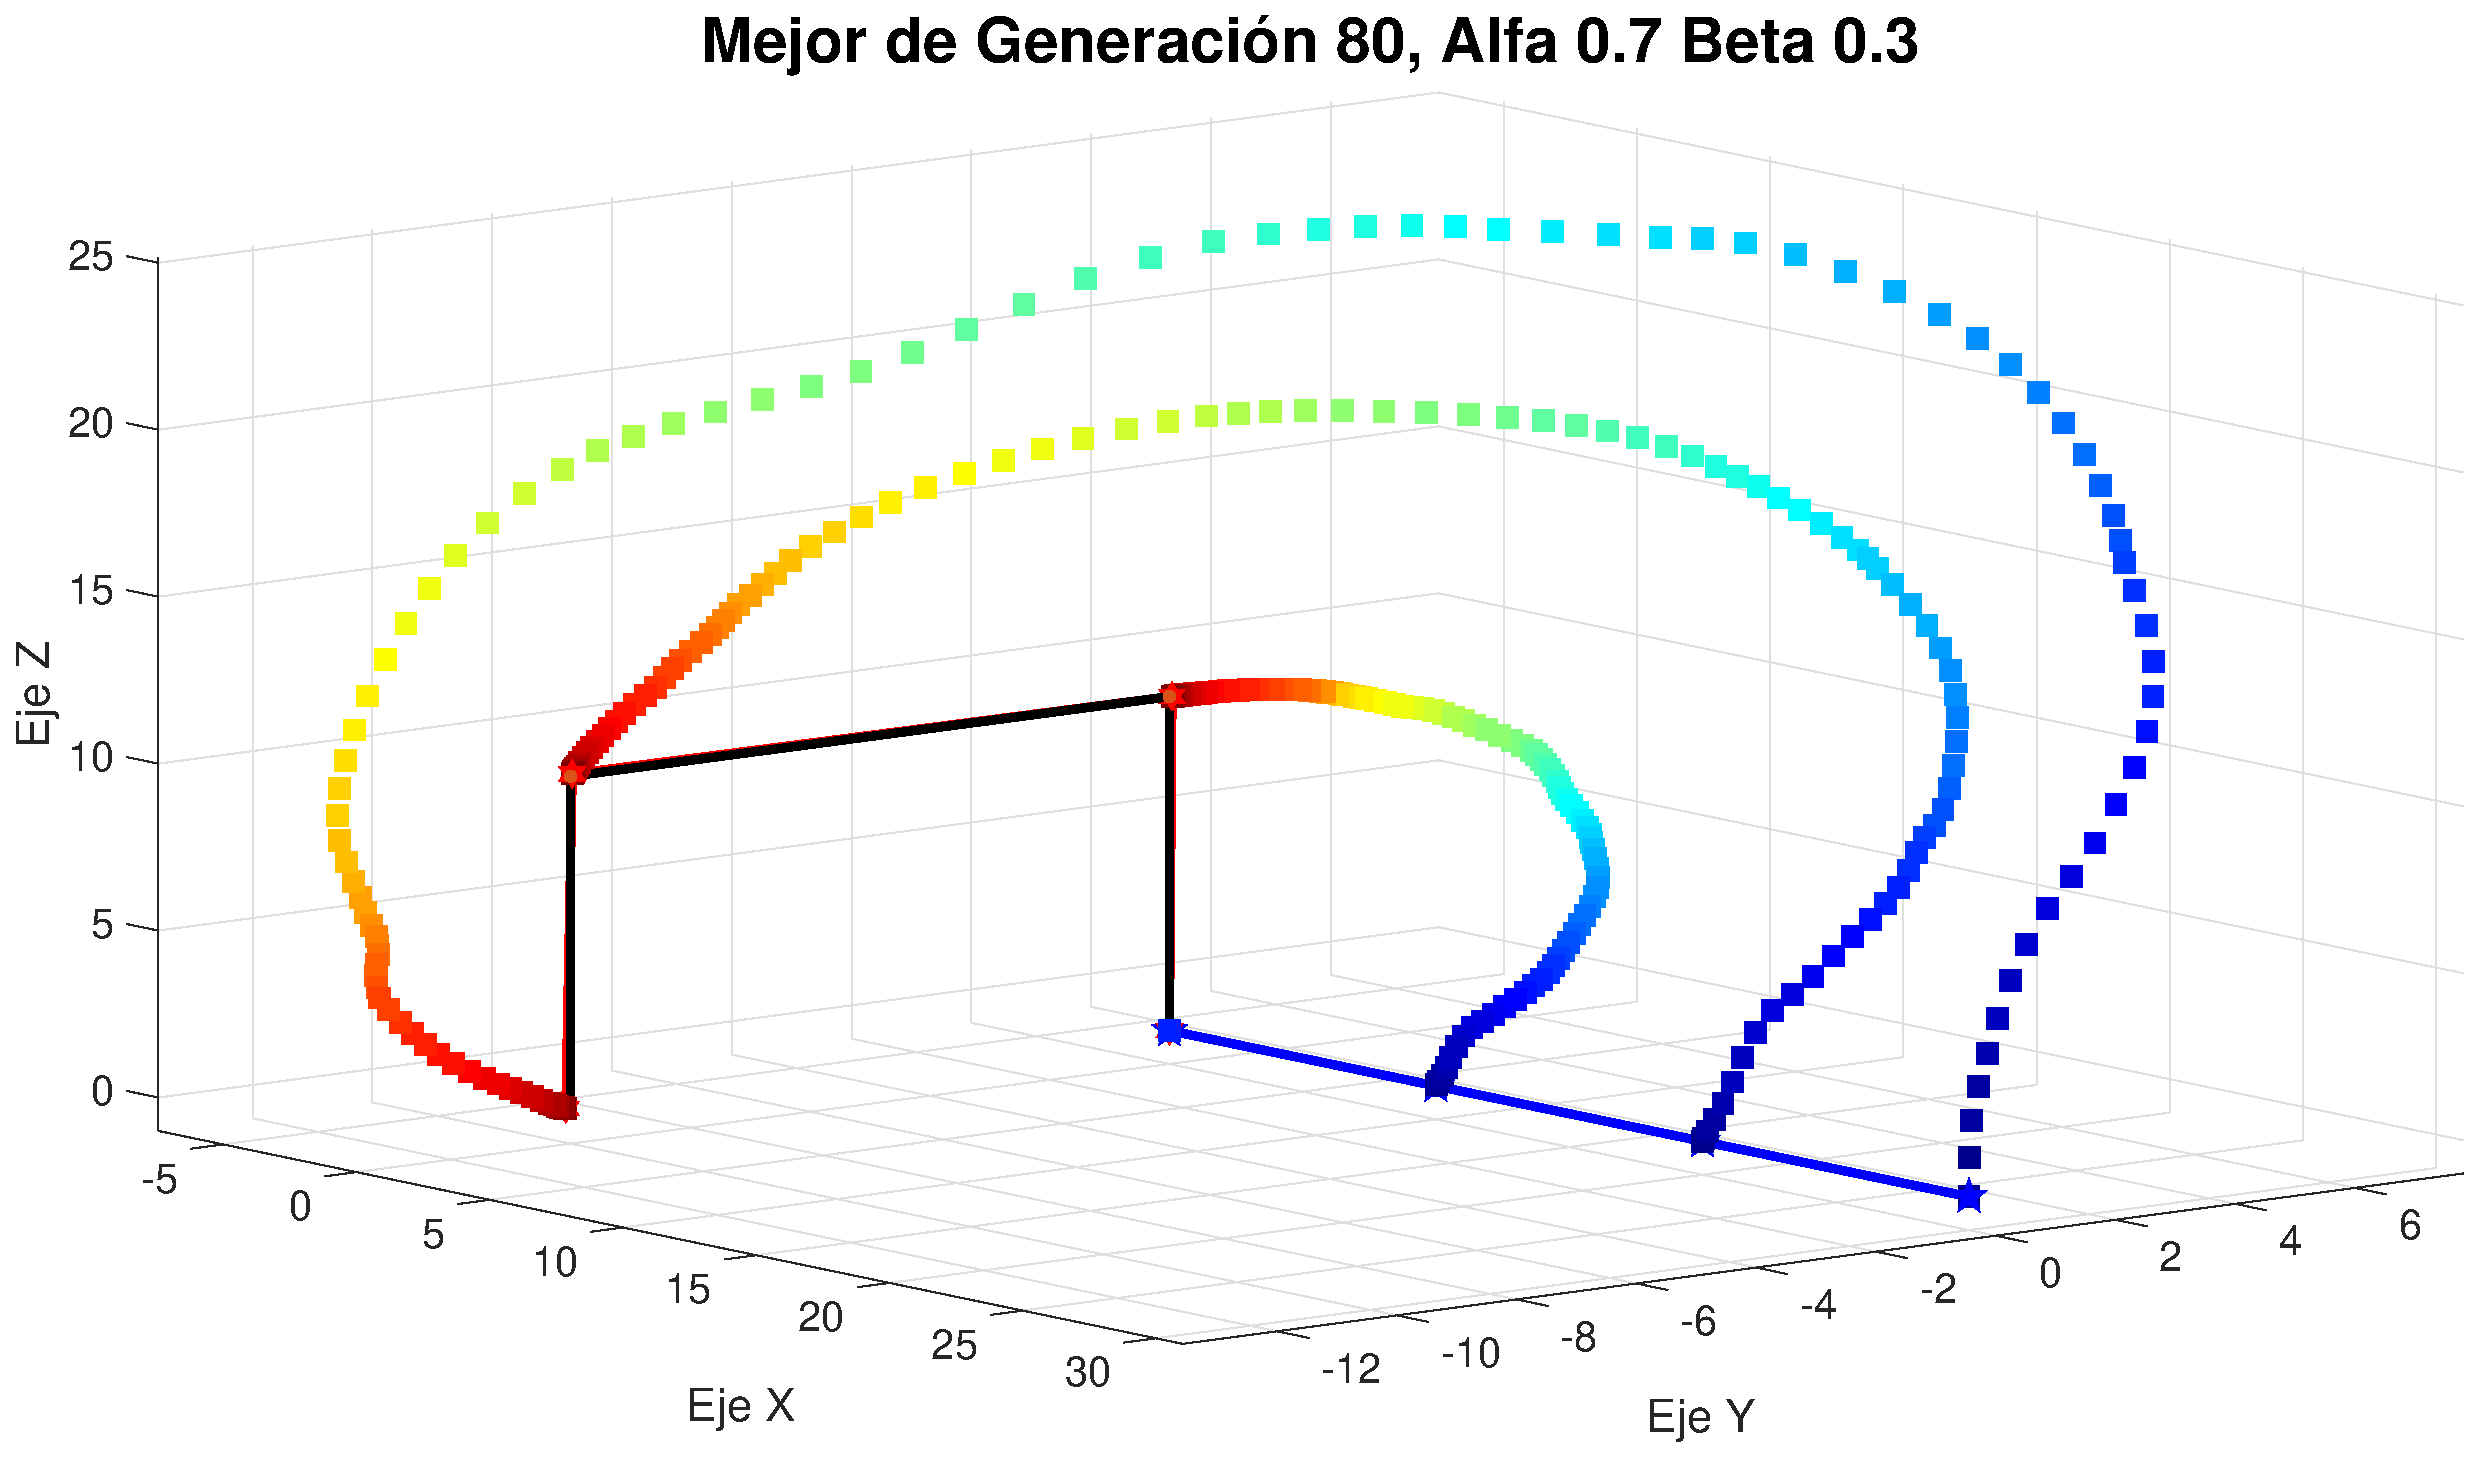
\includegraphics[width=4cm,height=2cm]{imag/VariacionAlfas/Alfa07Beta03.eps}}
\subfigure[$\alpha$: 0.8 y $\beta$: 0.2]{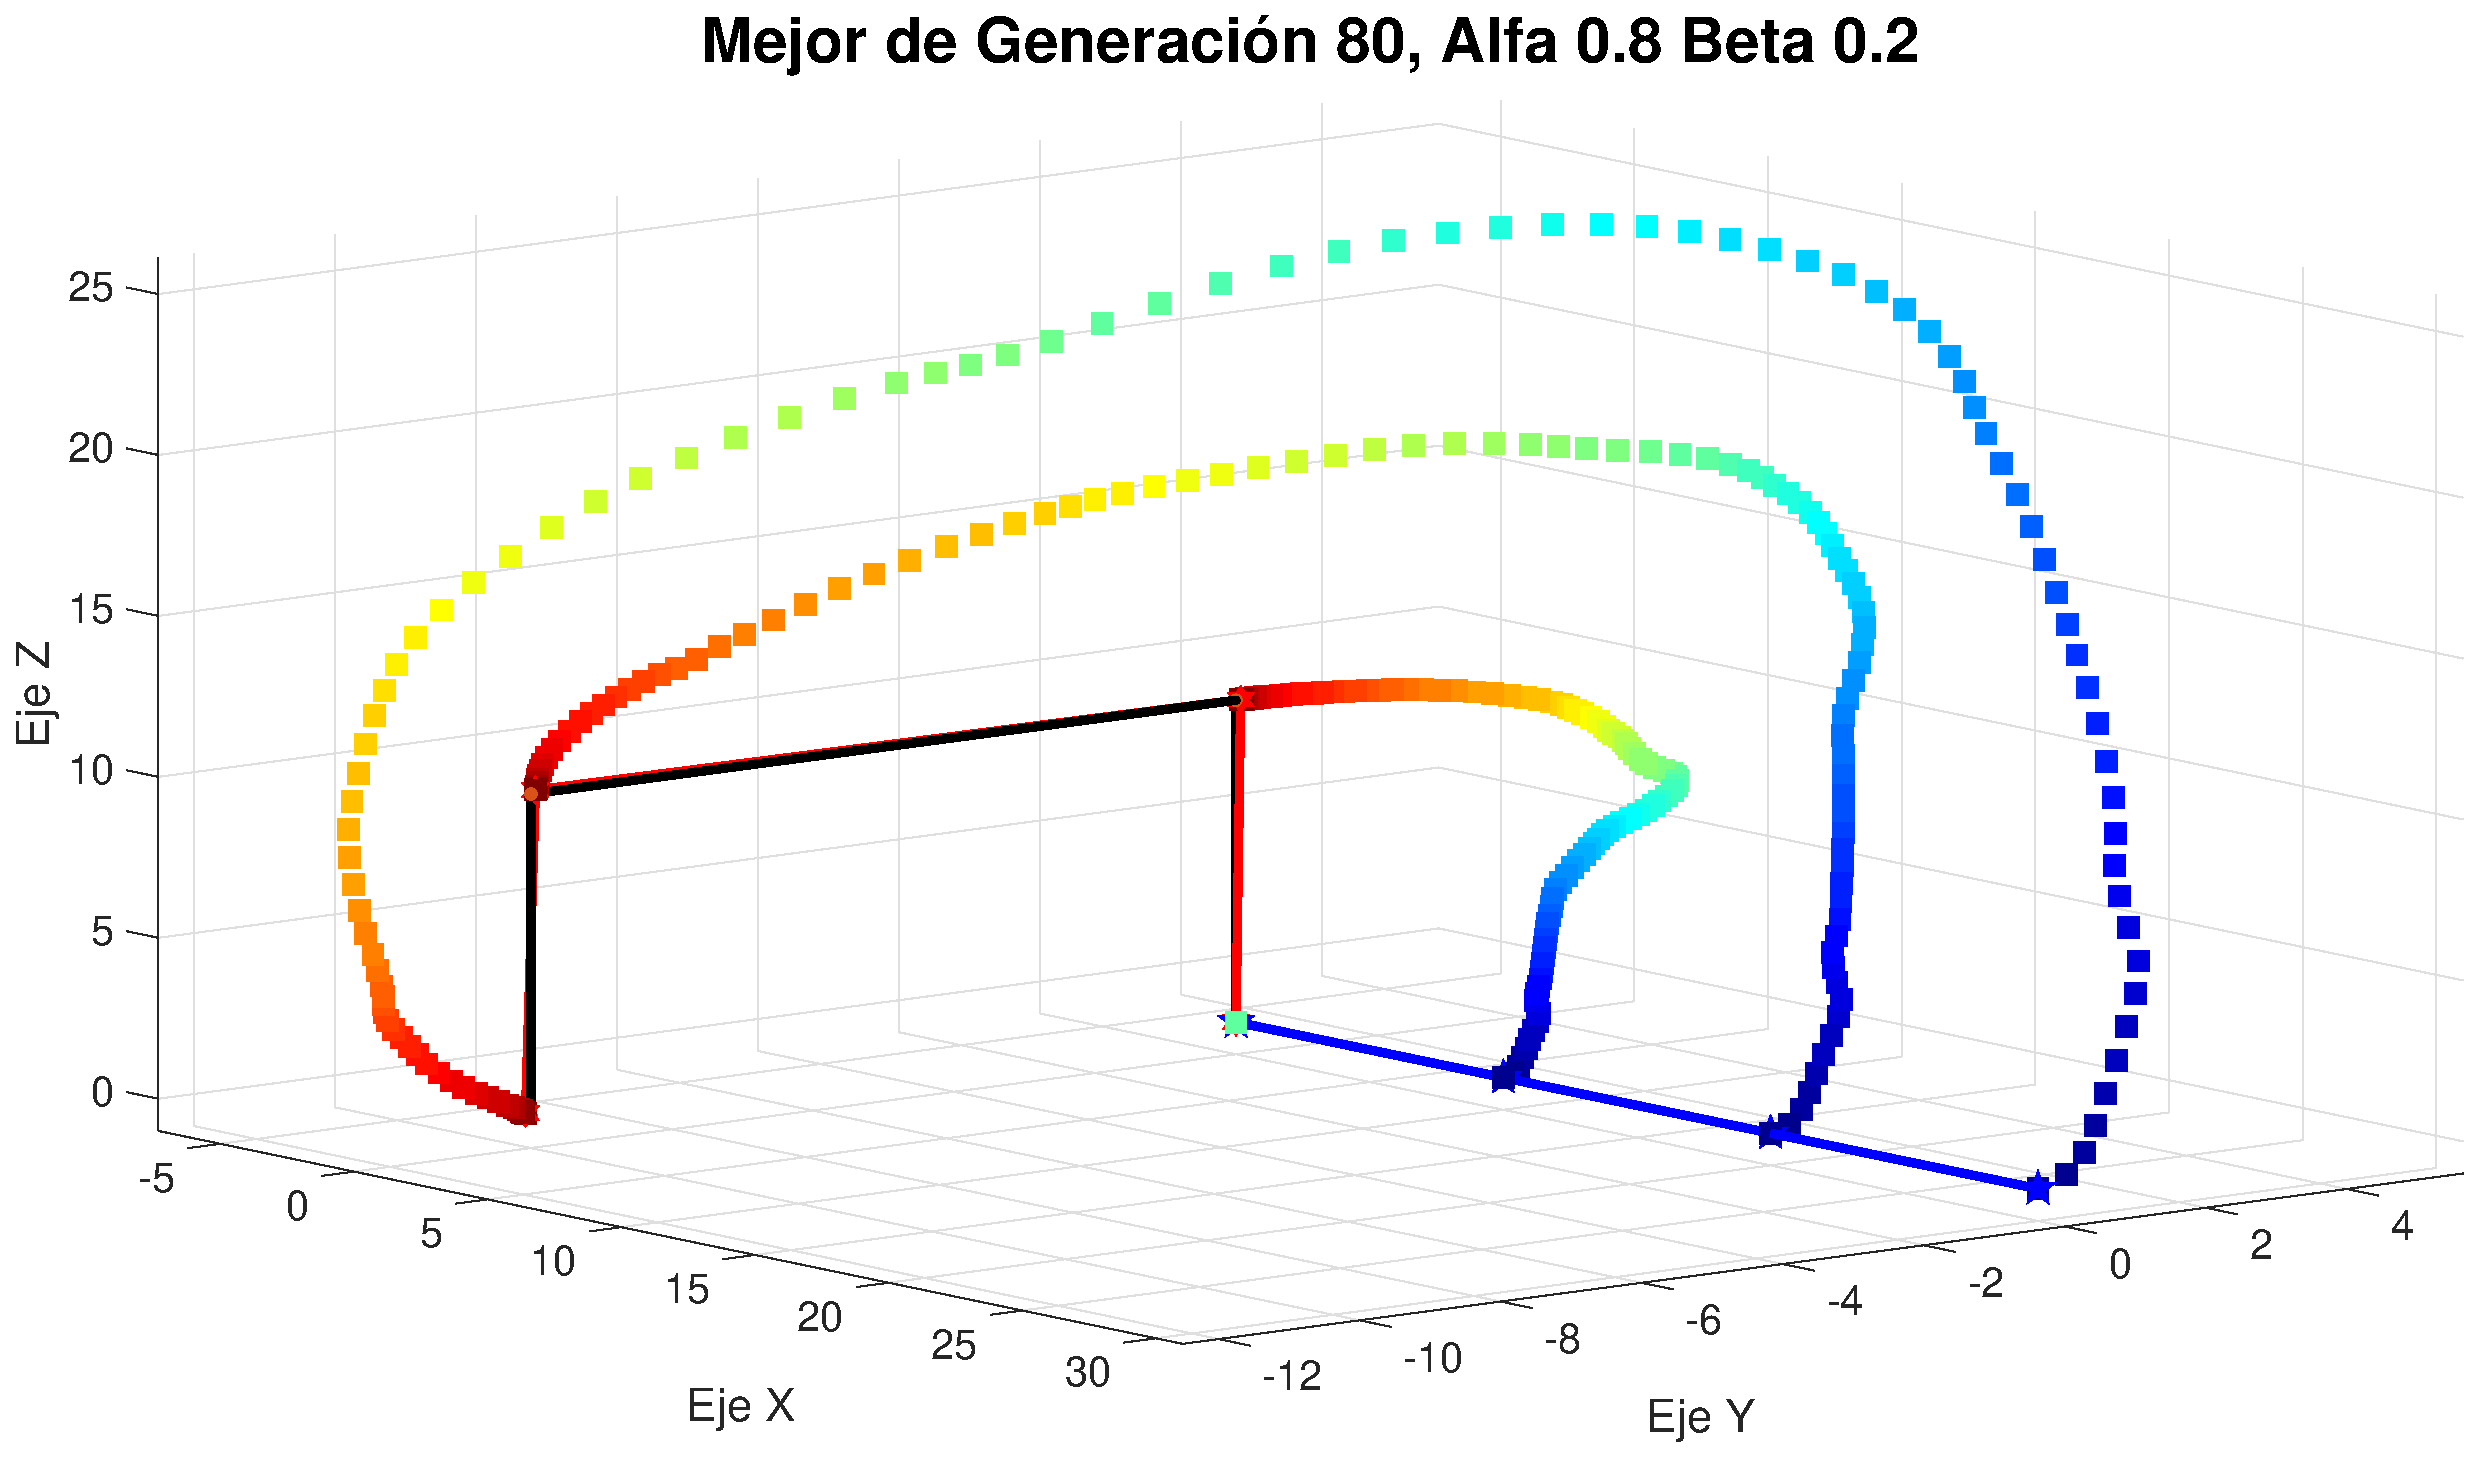
\includegraphics[width=4cm,height=2cm]{imag/VariacionAlfas/Alfa08Beta02.eps}}
\subfigure[$\alpha$: 0.9 y $\beta$: 0.1]{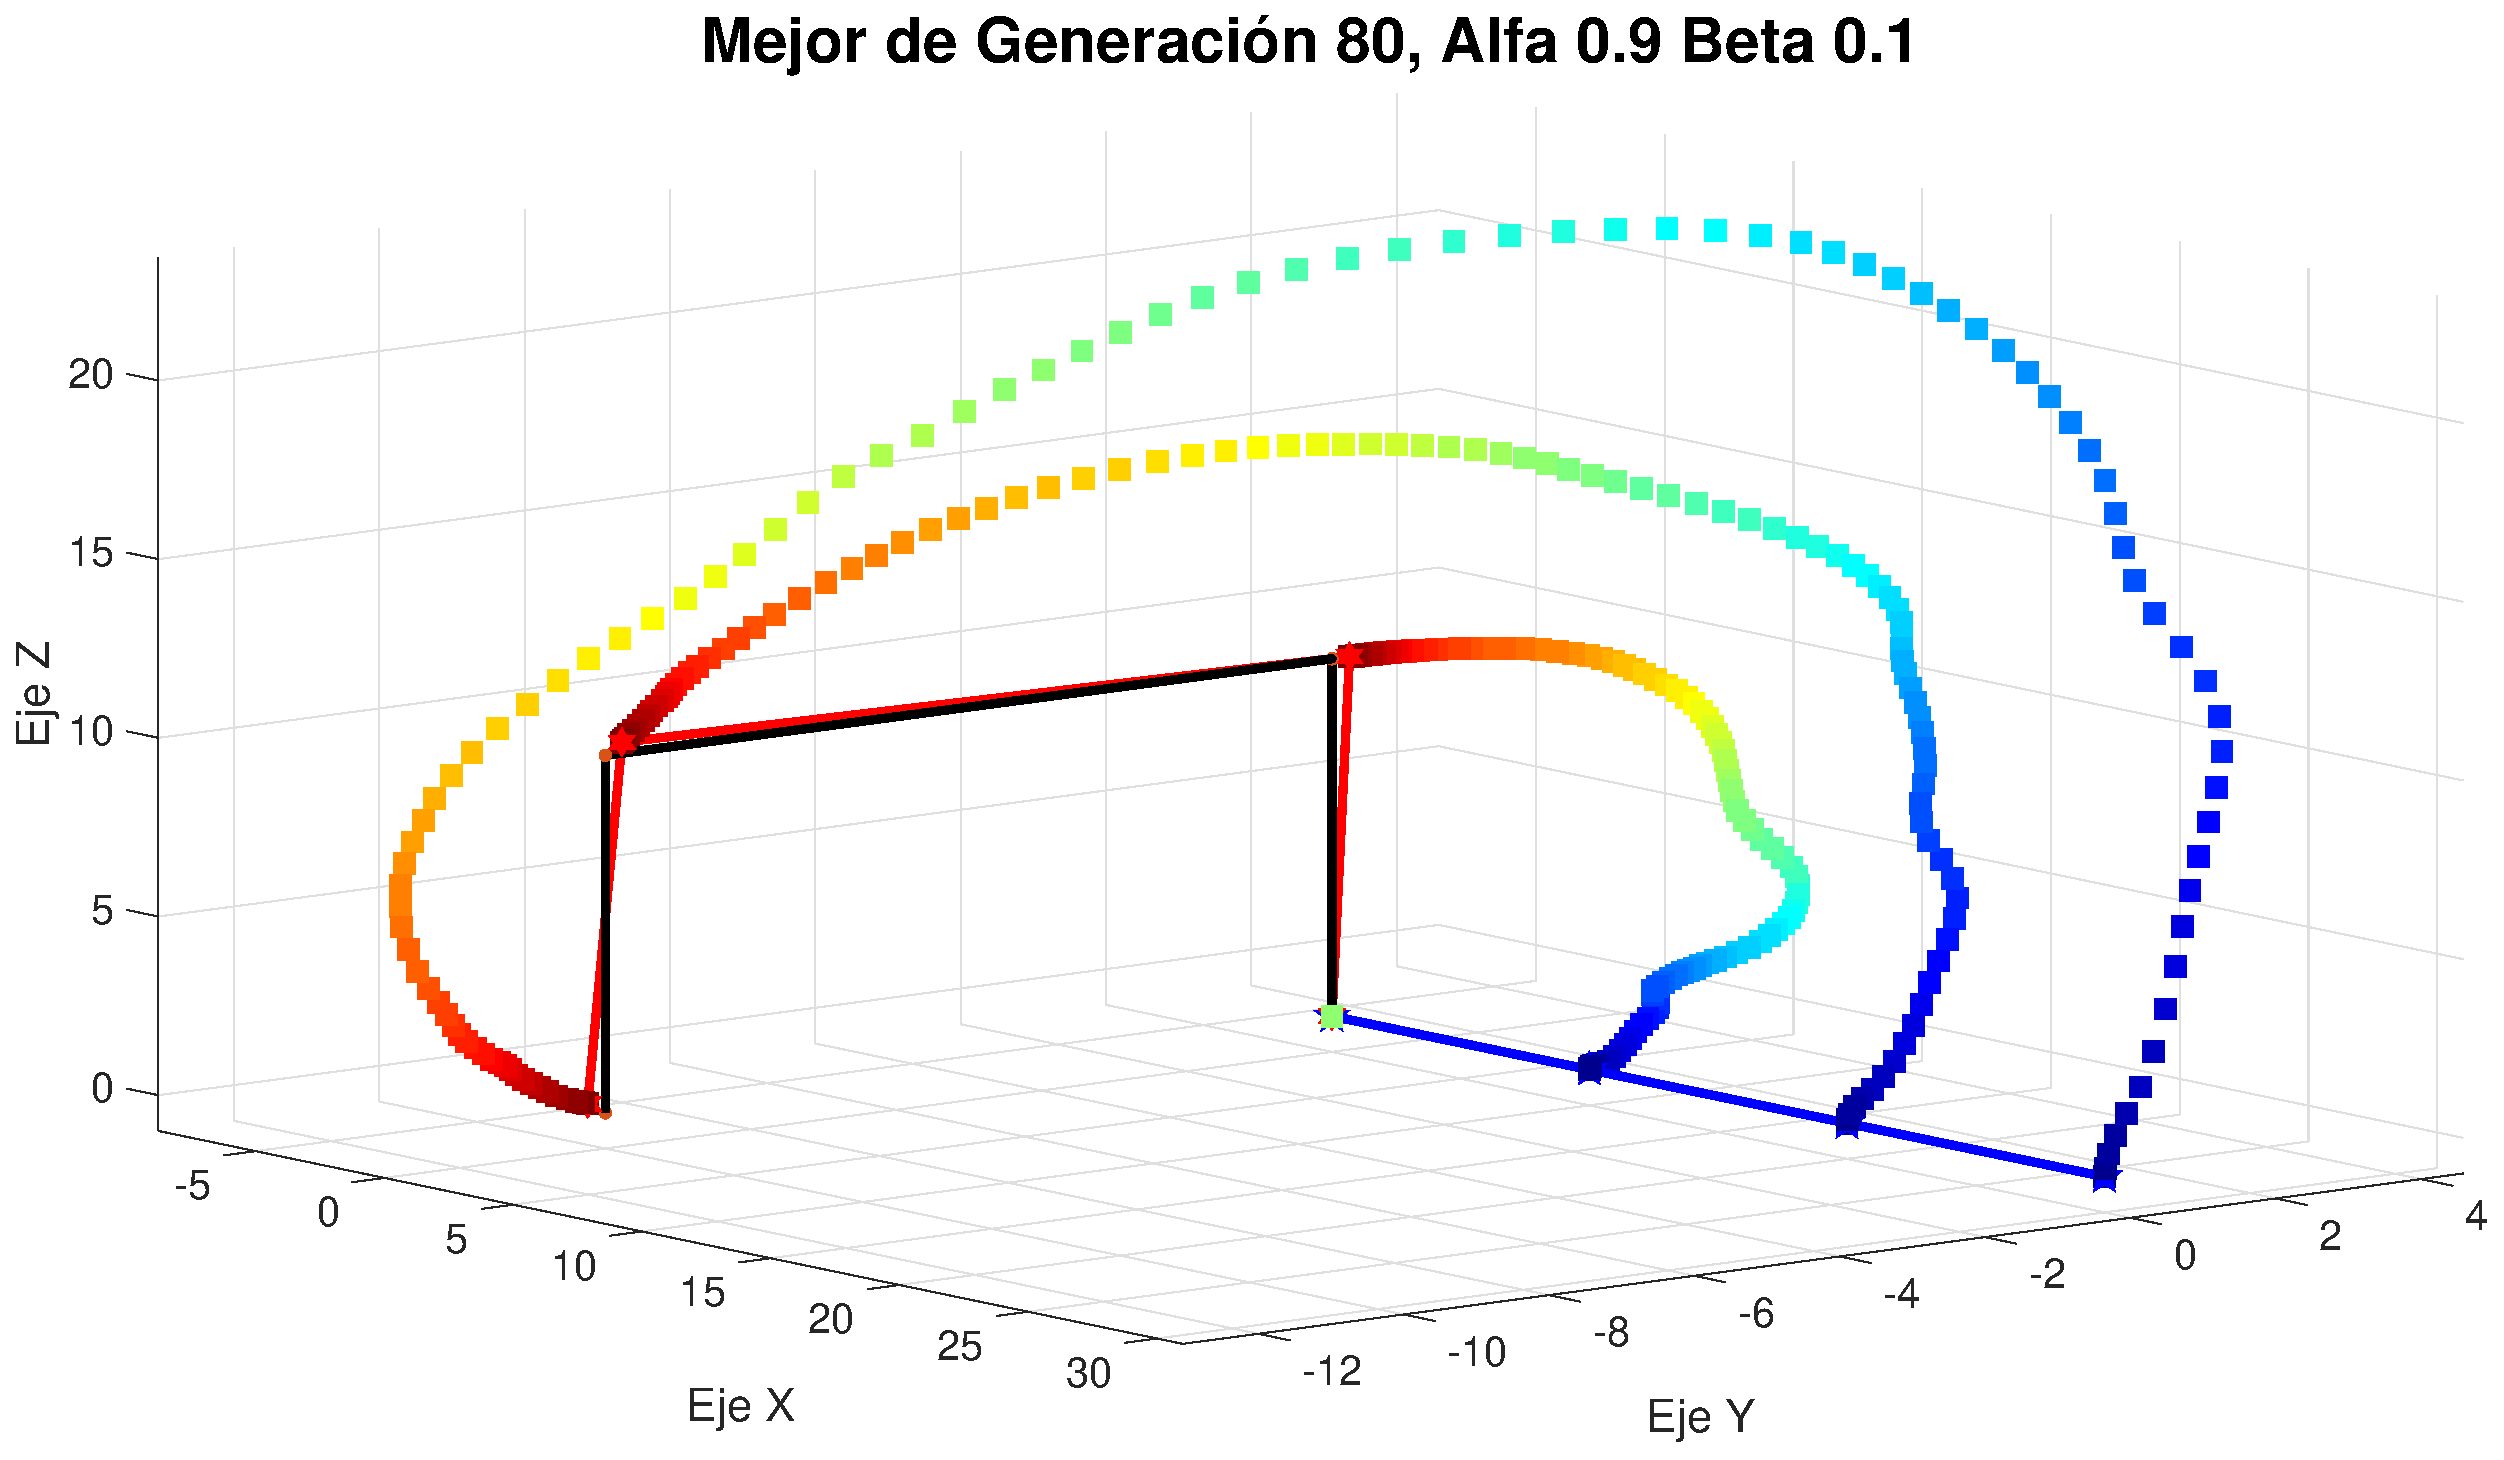
\includegraphics[width=4cm,height=2cm]{imag/VariacionAlfas/Alfa09Beta01.eps}}
\caption{Trayectoria del brazo con el mejor fitness para combinaciones de $\alpha$ y $\beta$.}
\label{Primresultados}
\end{figure}


\begin{figure}[h]
\centering
\subfigure[Fitness promedio.]{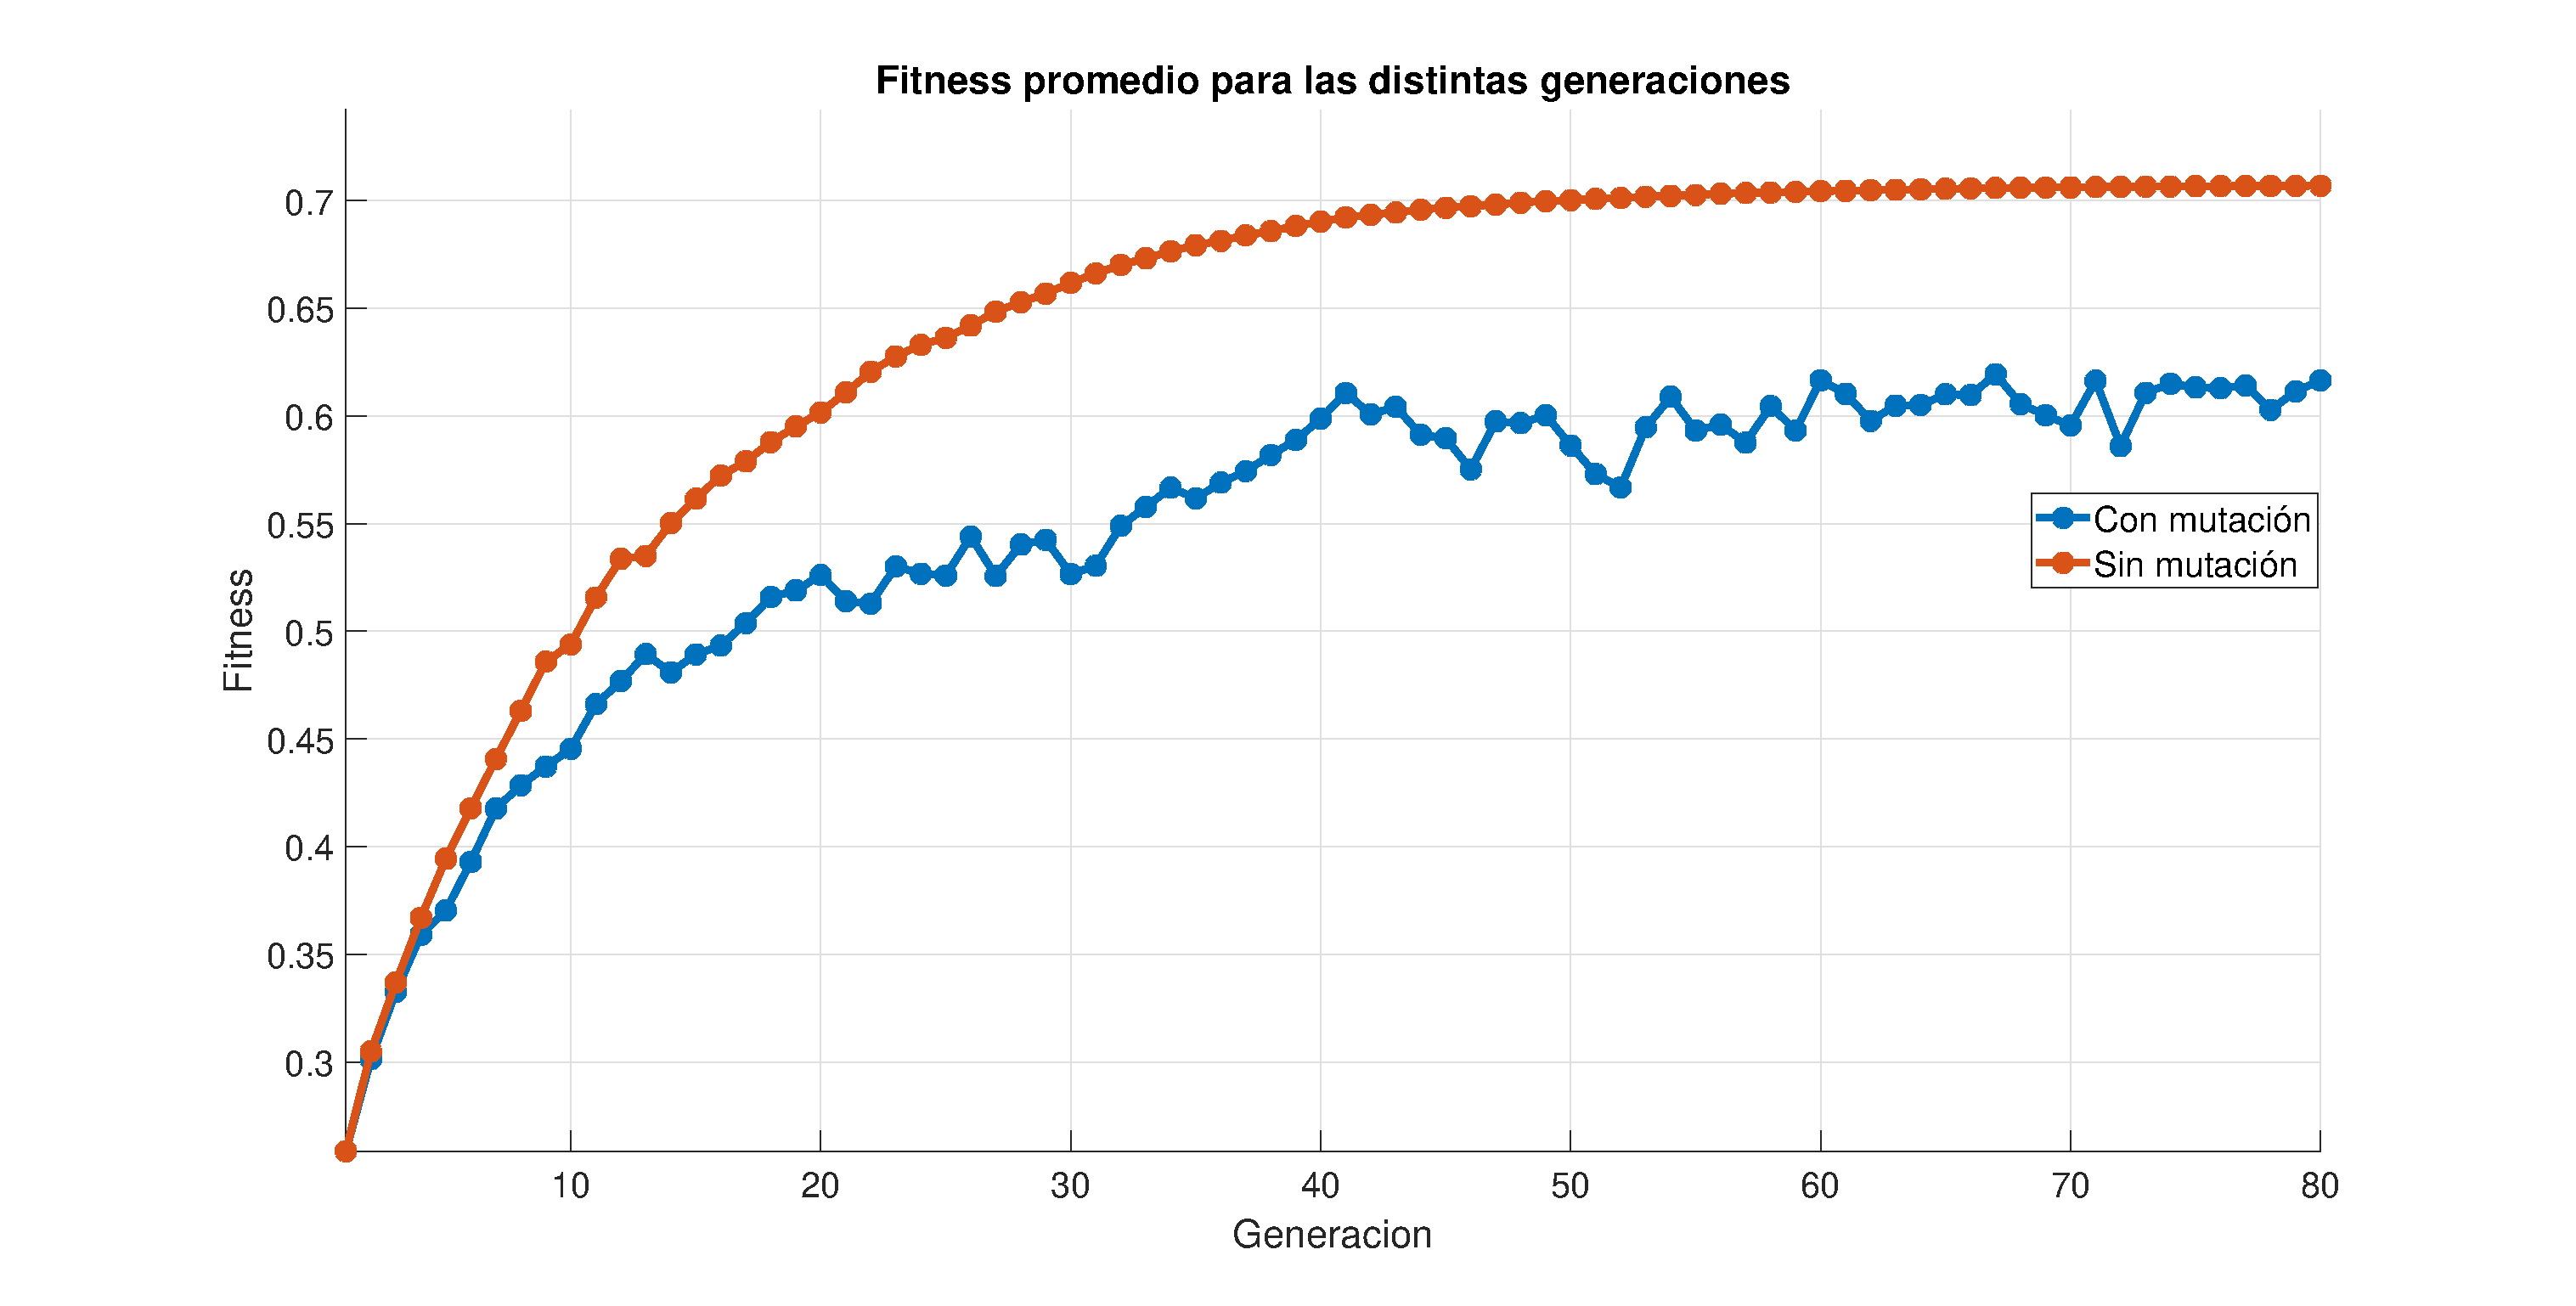
\includegraphics[width=7cm,height=3cm]{imag/versus/ComparaFitness.eps}}
\subfigure[Mejor fitness.]{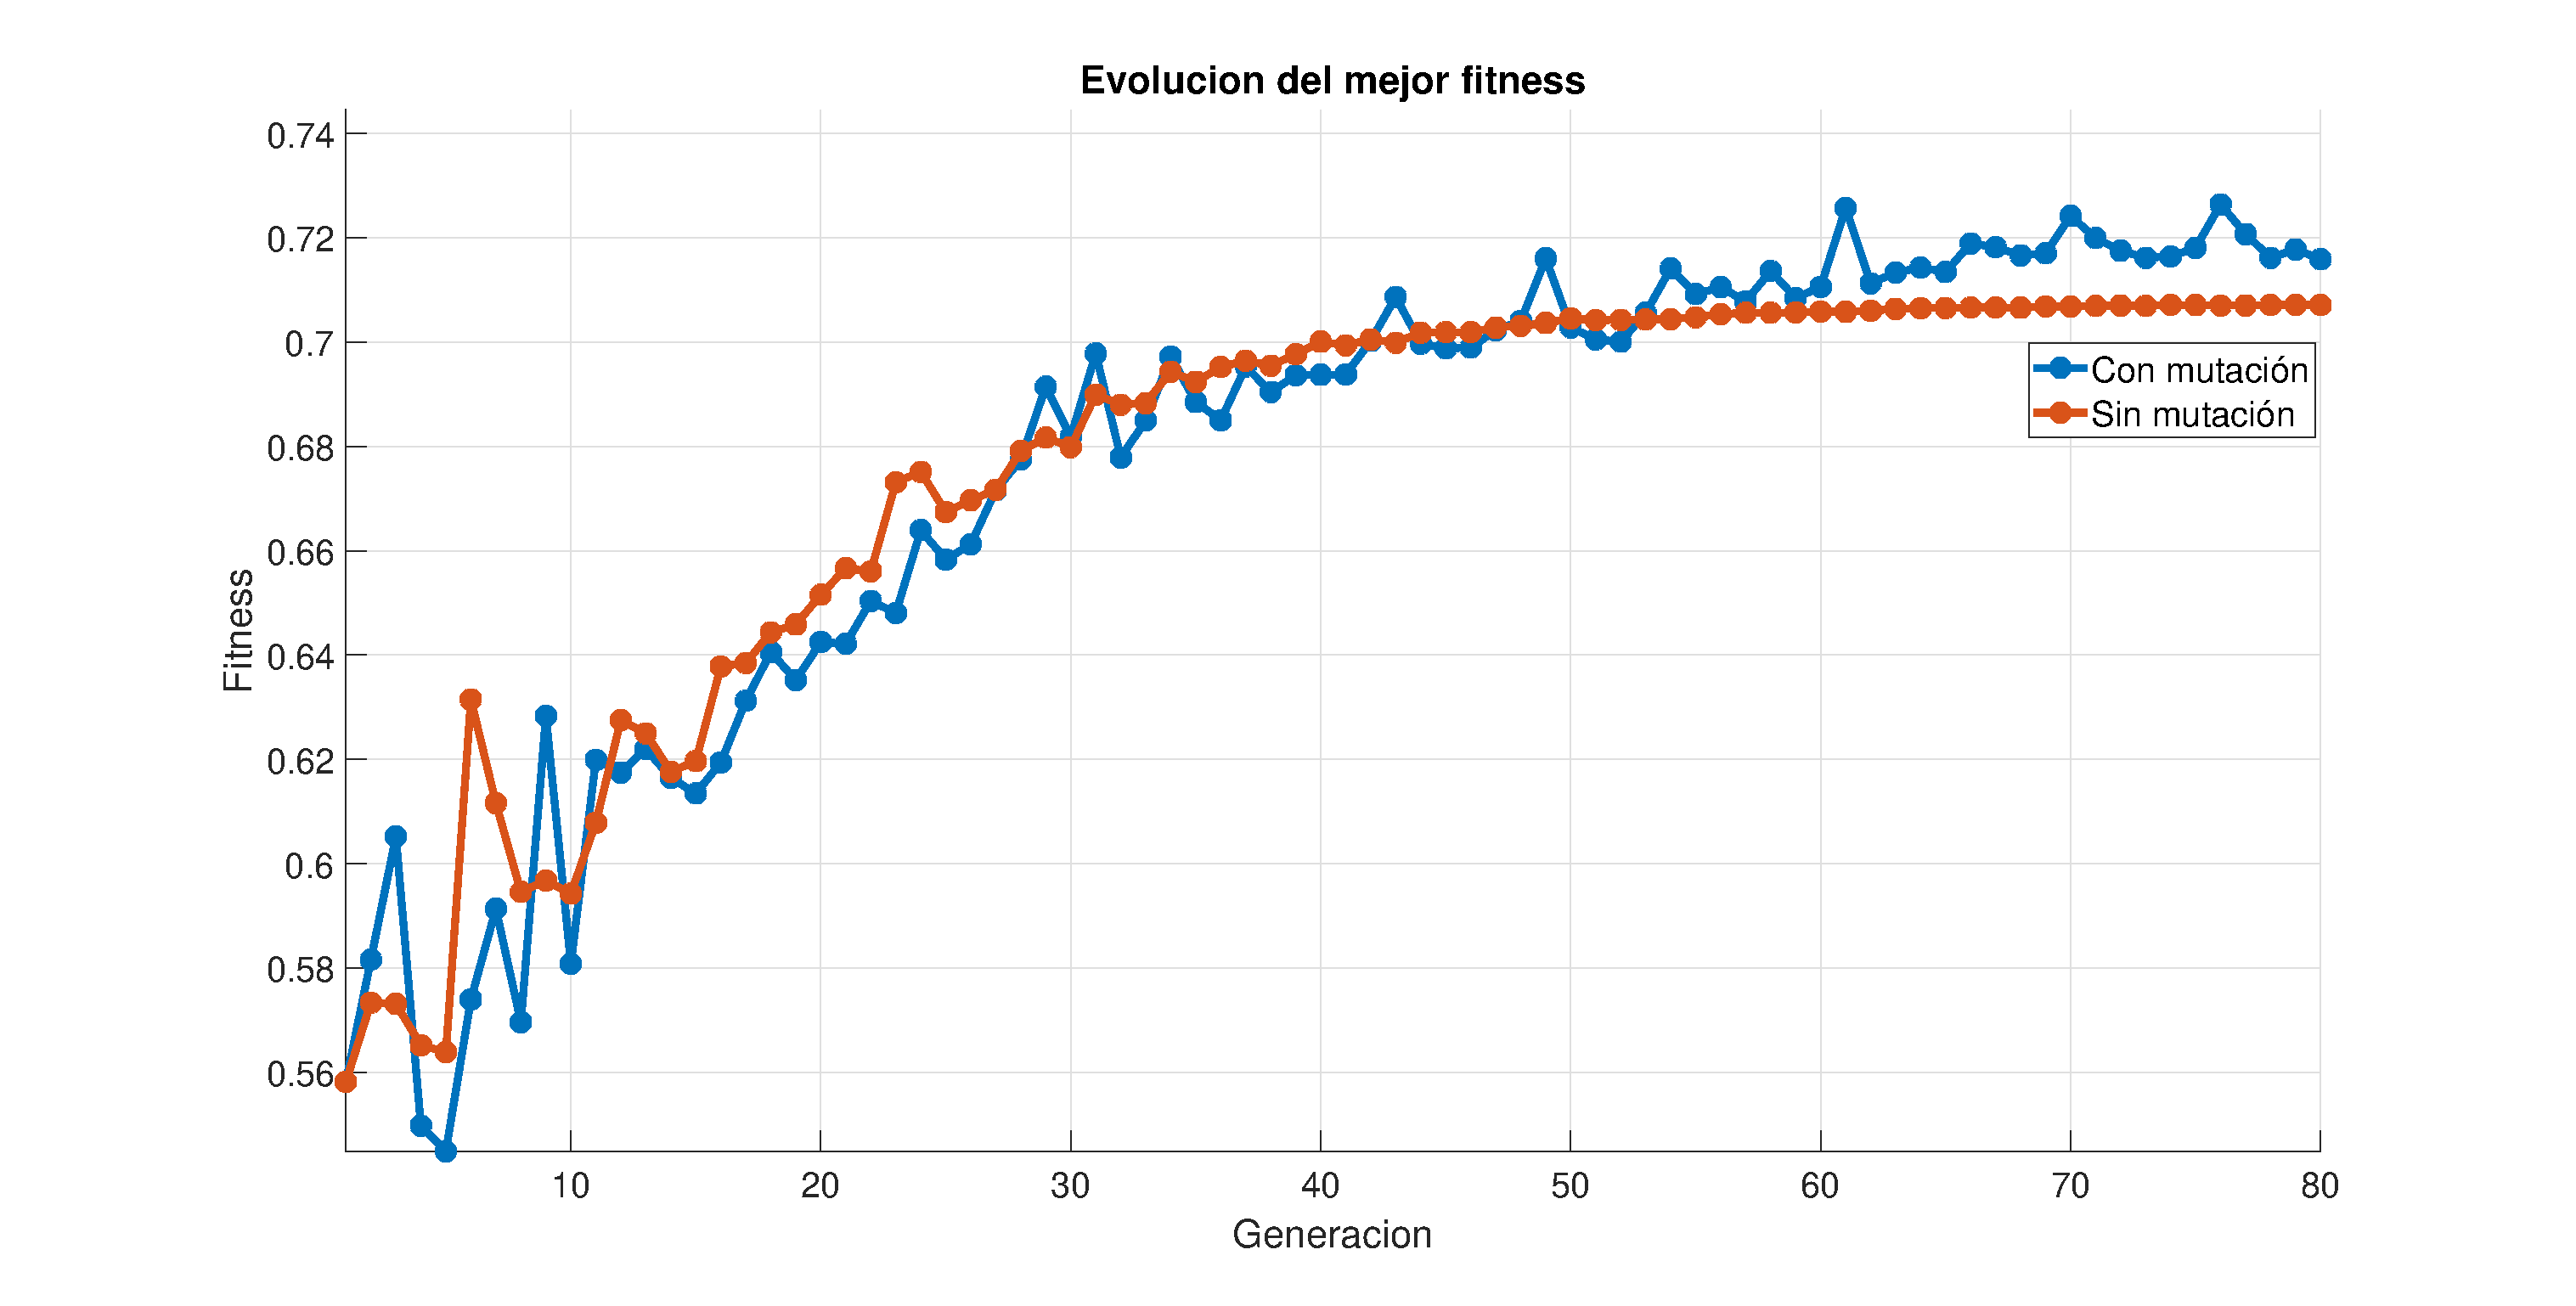
\includegraphics[width=7cm,height=3cm]{imag/versus/ComparaComparaFitness.eps}}
\subfigure[Error de posición.]{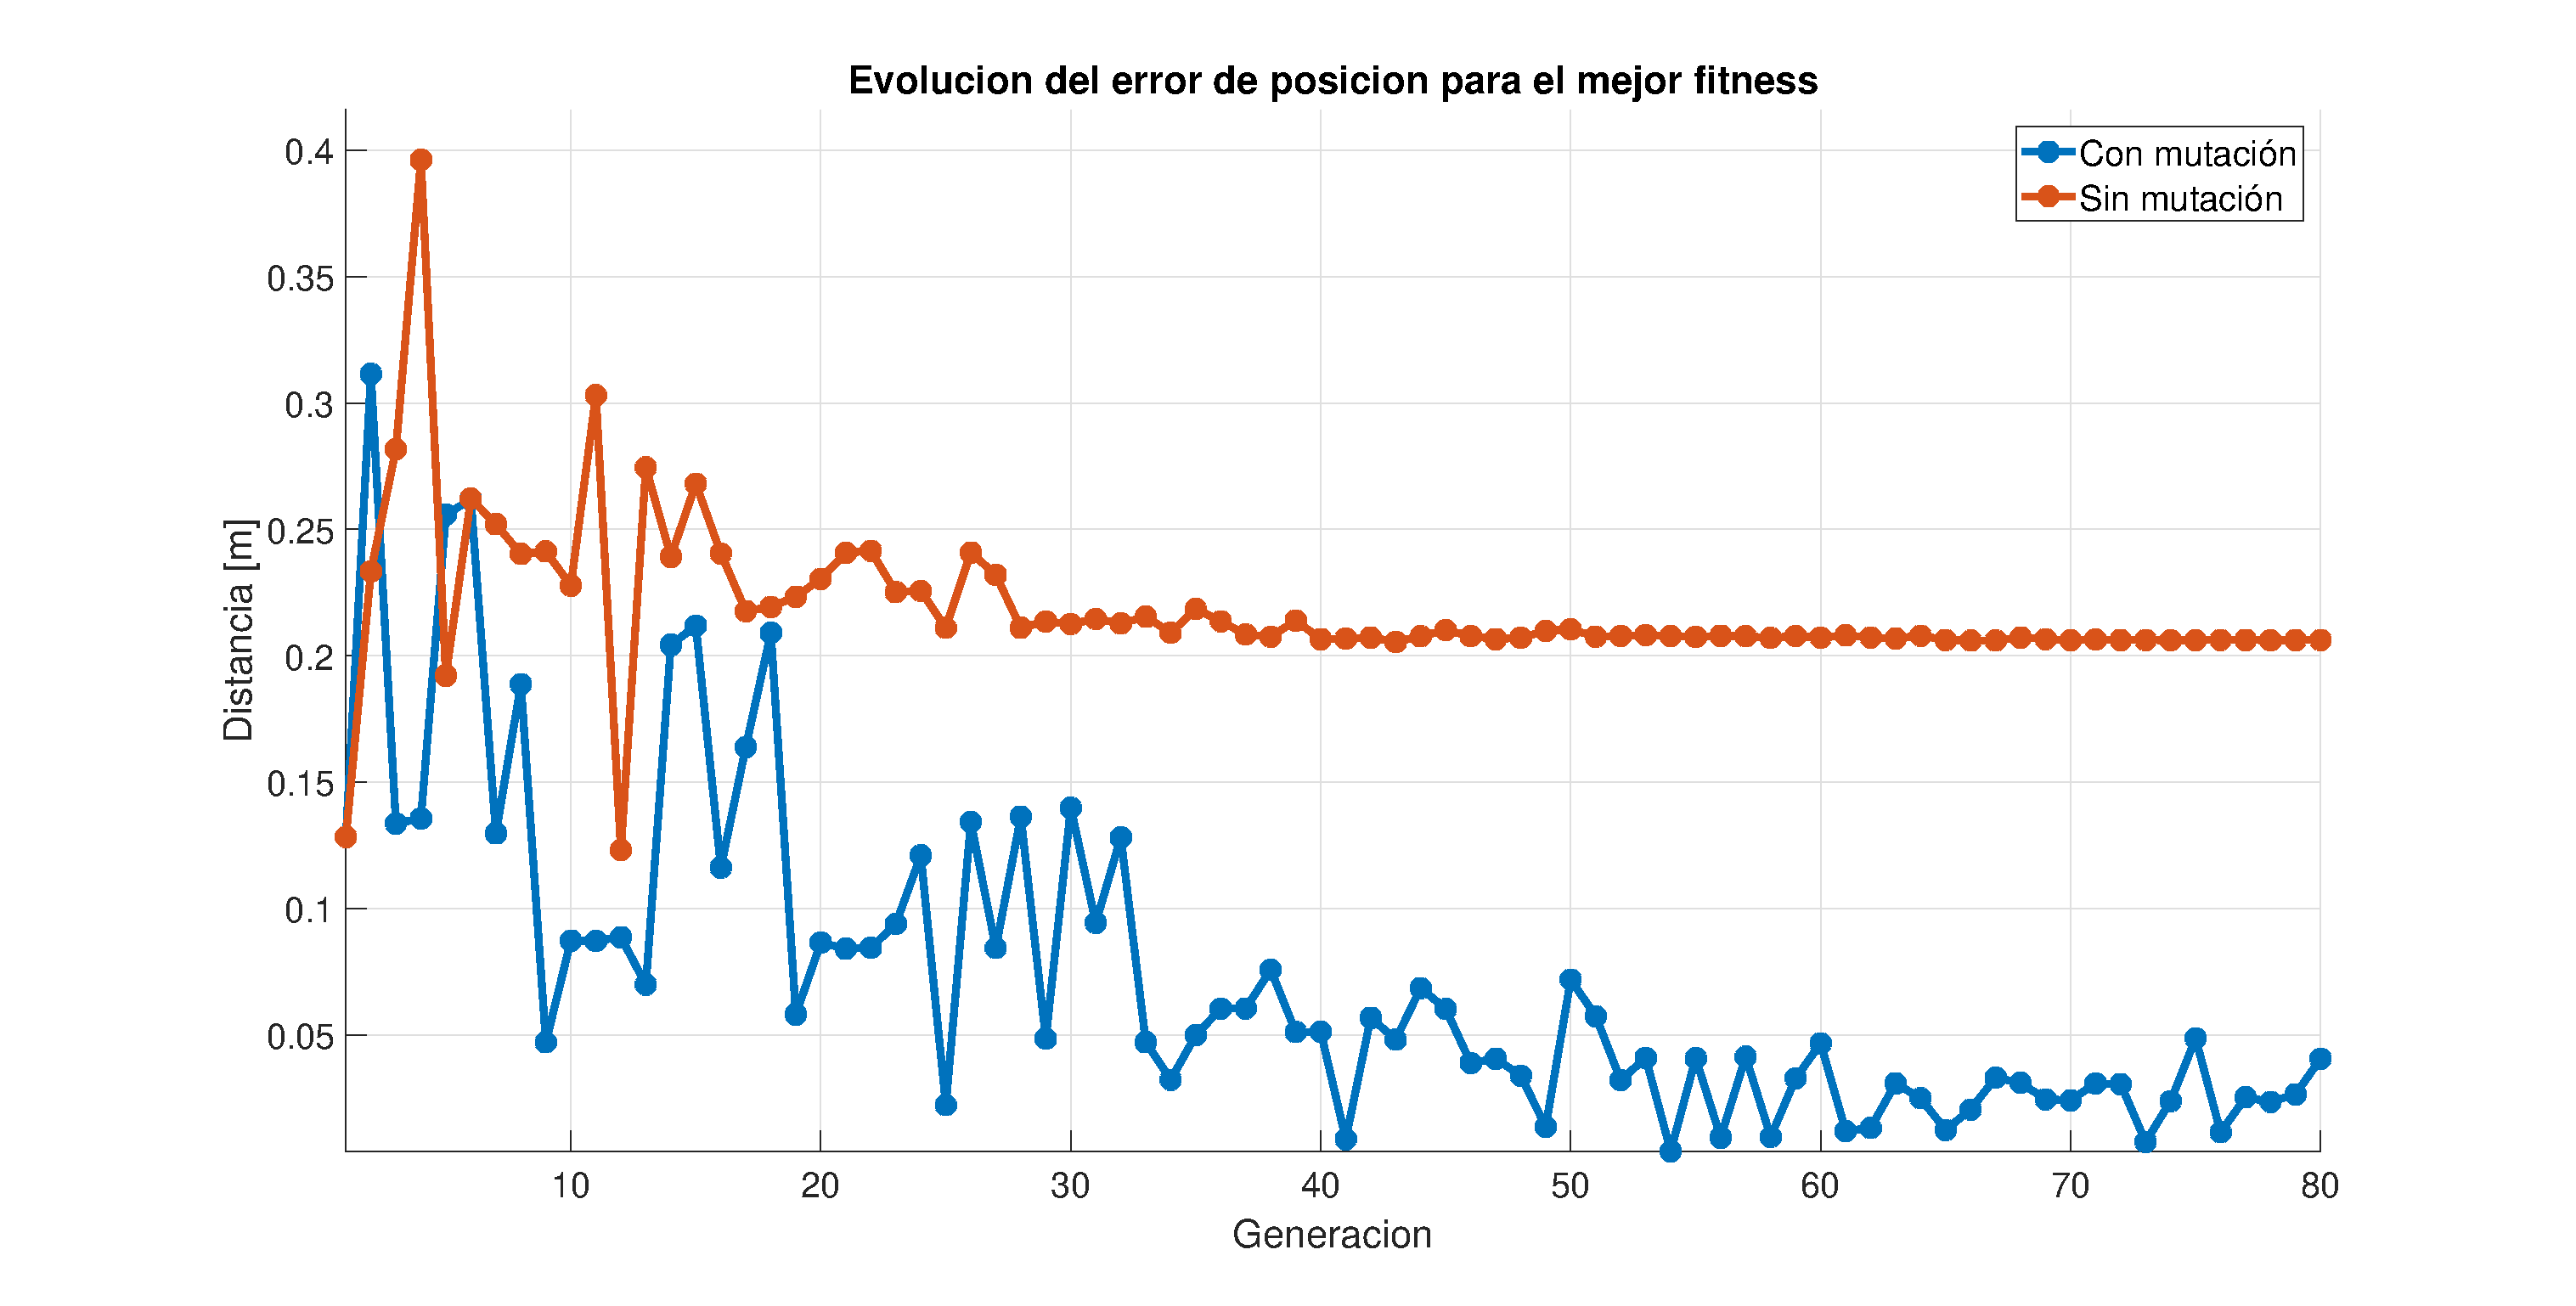
\includegraphics[width=14cm,height=3cm]{imag/versus/ComparaErrorPosicion.eps}}
\caption{Evolución de los resultados con y sin mutaciones para un $\alpha$: 0.5 y $\beta$: 0.5.}
\label{esosososs}
\end{figure}
\section{Resultados}

Cuando se realizaron experimentos preliminares en donde solo se penalizaba la distancia del brazo al punto objetivo, los resultados mostraban un comportamiento similar al de la figura \ref{smoothness} en donde la ubicación geométrica de cada muestra se encontraba muy separada, es decir, su velocidad era muy grande. Esto se soluciona al incorporar una penalización en la velocidad y creando un nuevo fitness como se muestra en la ecuación \eqref{fitness}. La selección de los hiperparámetros $\alpha$ y $\beta$ del fitness, se ajustan experimentalmente logrando los resultados de las figuras \ref{muchas} y \ref{Primresultados}. Se puede notar que si el valor de $\alpha$ es pequeño, el fitness es cada vez mejor y la distancia al punto objetivo es cada vez más pequeña. Sin embargo, dejar con muy poca penalización la velocidad conlleva problemas relacionados a la separación de las muestras, que al ser en exceso requerirá de mayor torque en los motores actuadores, por otro lado, si $\alpha$ es pequeño el movimiento no es tan suave y nacen curvas bruscas que cambian de una muestra a otra como se ve en la figura \ref{Primresultados}(a), (b) y (c). Por otro lado, si $\beta$ es pequeño (penalizando de menor manera la posición final), se puede ver en la figura \ref{Primresultados}(i) que la punto del brazo no es capaz de llegar al objetivo y el fitness promedio es menor. De esta manera se selecciono valores medio igual a 0.5, para evitar los problemas de ambos extremos. \\
Luego de haber seleccionados los mejores individuos y generar el crossover, el sistema realiza la pregunta lógica de si crear o no la mutación. Cuando el sistema no realiza mutación se presenta el conocido problema de estancamiento en los resultados como muestra la figura \ref{esosososs}. Esto cambia cuando el sistema tiene la opción de aplicar mutación, donde, a pesar que el mejor fitness de las generaciones no varia mucho (figura \ref{esosososs}(b)) en comparación al no usar mutación, si se notaron cambios importantes en la distancia que tiene la punta del brazo con el objetivo. Sin embargo, cabe mencionar que si el valor del porcentaje de mutación es muy alto, el sistema se comparta de manera errática, por lo tanto se recomienda utilizar valores pequeños de mutación no mayores al $10\%$.\\
Finalmente, respecto a los resultados finales se lograron los objetivos mencionados, logrando que el brazo llegara a su objetivo con bajas velocidades. Esto se puede ver en la Figura \ref{lalalalalal} donde se muestran los cambios generados durante las generaciones. En la figura \ref{lalalalalal}(b) y (d) se puede ver el contraste en usar o no la mutación, ya que cuando se analiza el peor caso sin mutación, el resultado no es tan malo ni tan alejado del mejor. Por otro lado, si se usa mutación, cambia completamente el peor escenario, desfavoreciendo incluso la distancia final del brazo hacia el objetivo. Por el contrario, si se analiza el mejor caso de las generaciones, se ve claramente la ventaja de usar mutación mostrando en la figura \ref{lalalalalal}(a) que llega casi completamente al objetivo mientras que en la figura \ref{lalalalalal}(c) no logra llegar completamente.


\begin{figure}
\centering
\subfigure[Mejor trayectoria con mutación.]{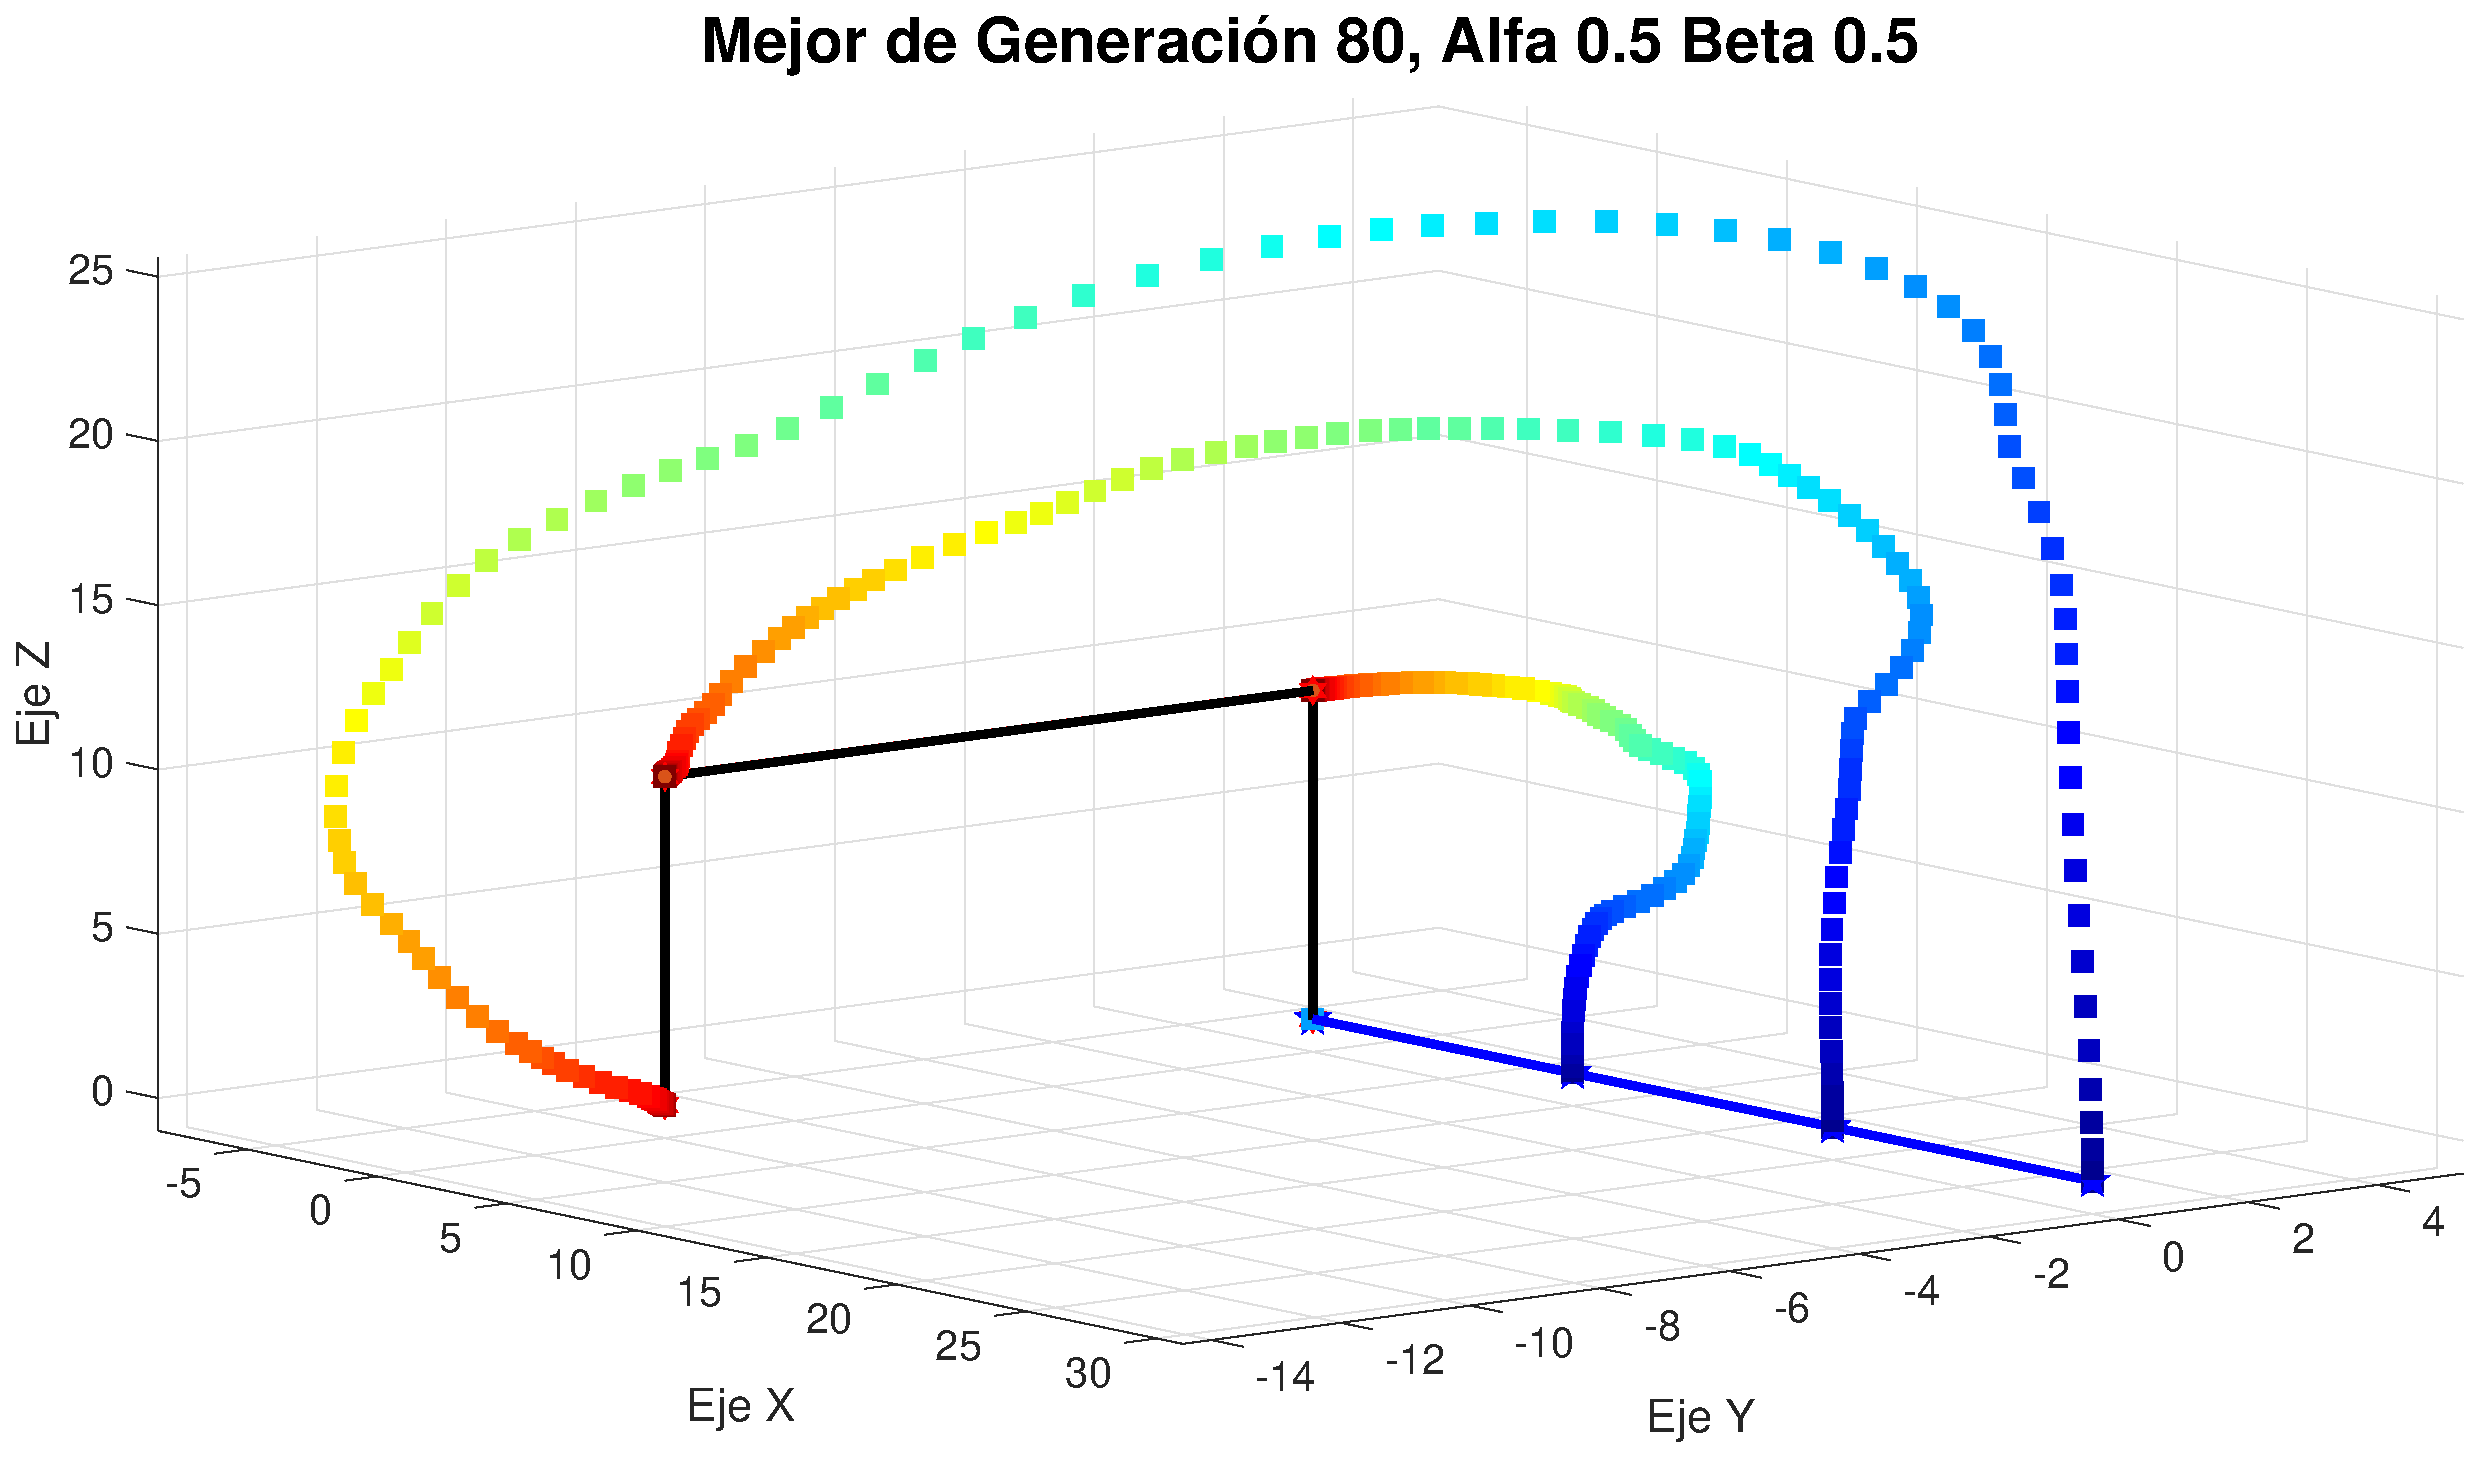
\includegraphics[width=7cm,height=3cm]{imag/versus/MejorConMutacion.eps}}
\subfigure[Peor trayectoria con mutación.]{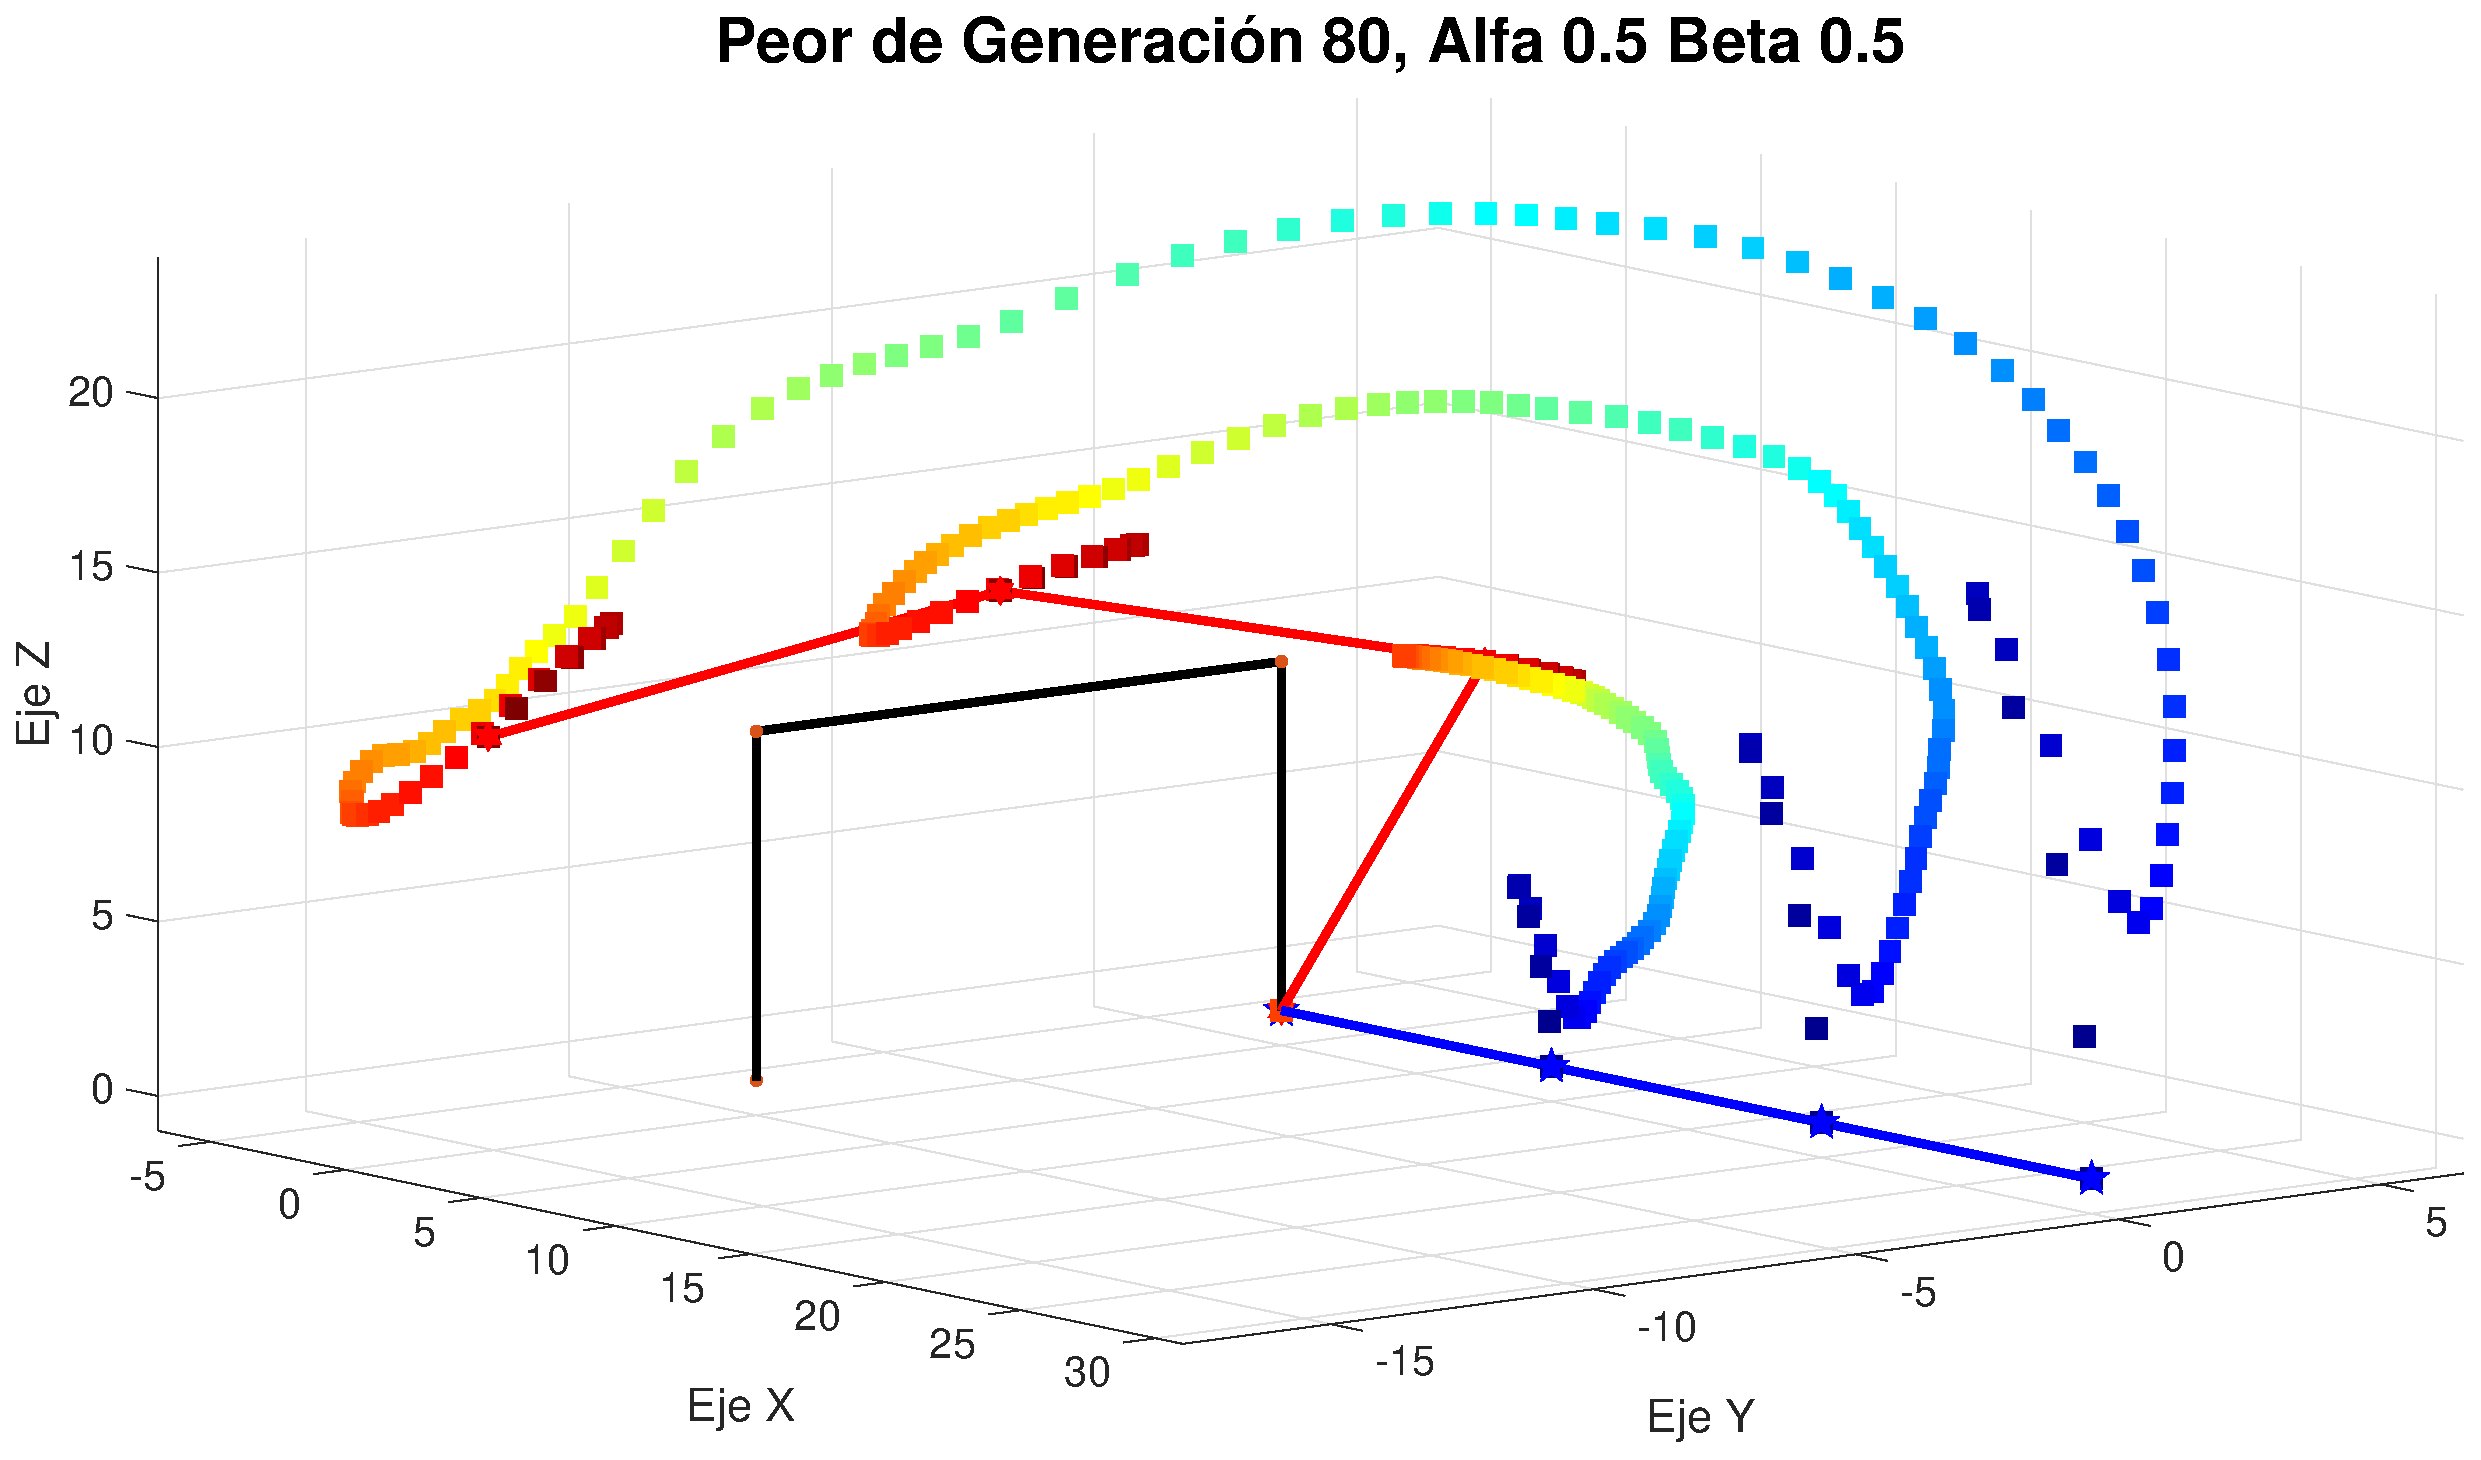
\includegraphics[width=7cm,height=3cm]{imag/versus/PeorConMutacion.eps}}
\subfigure[Mejor trayectoria sin mutación.]{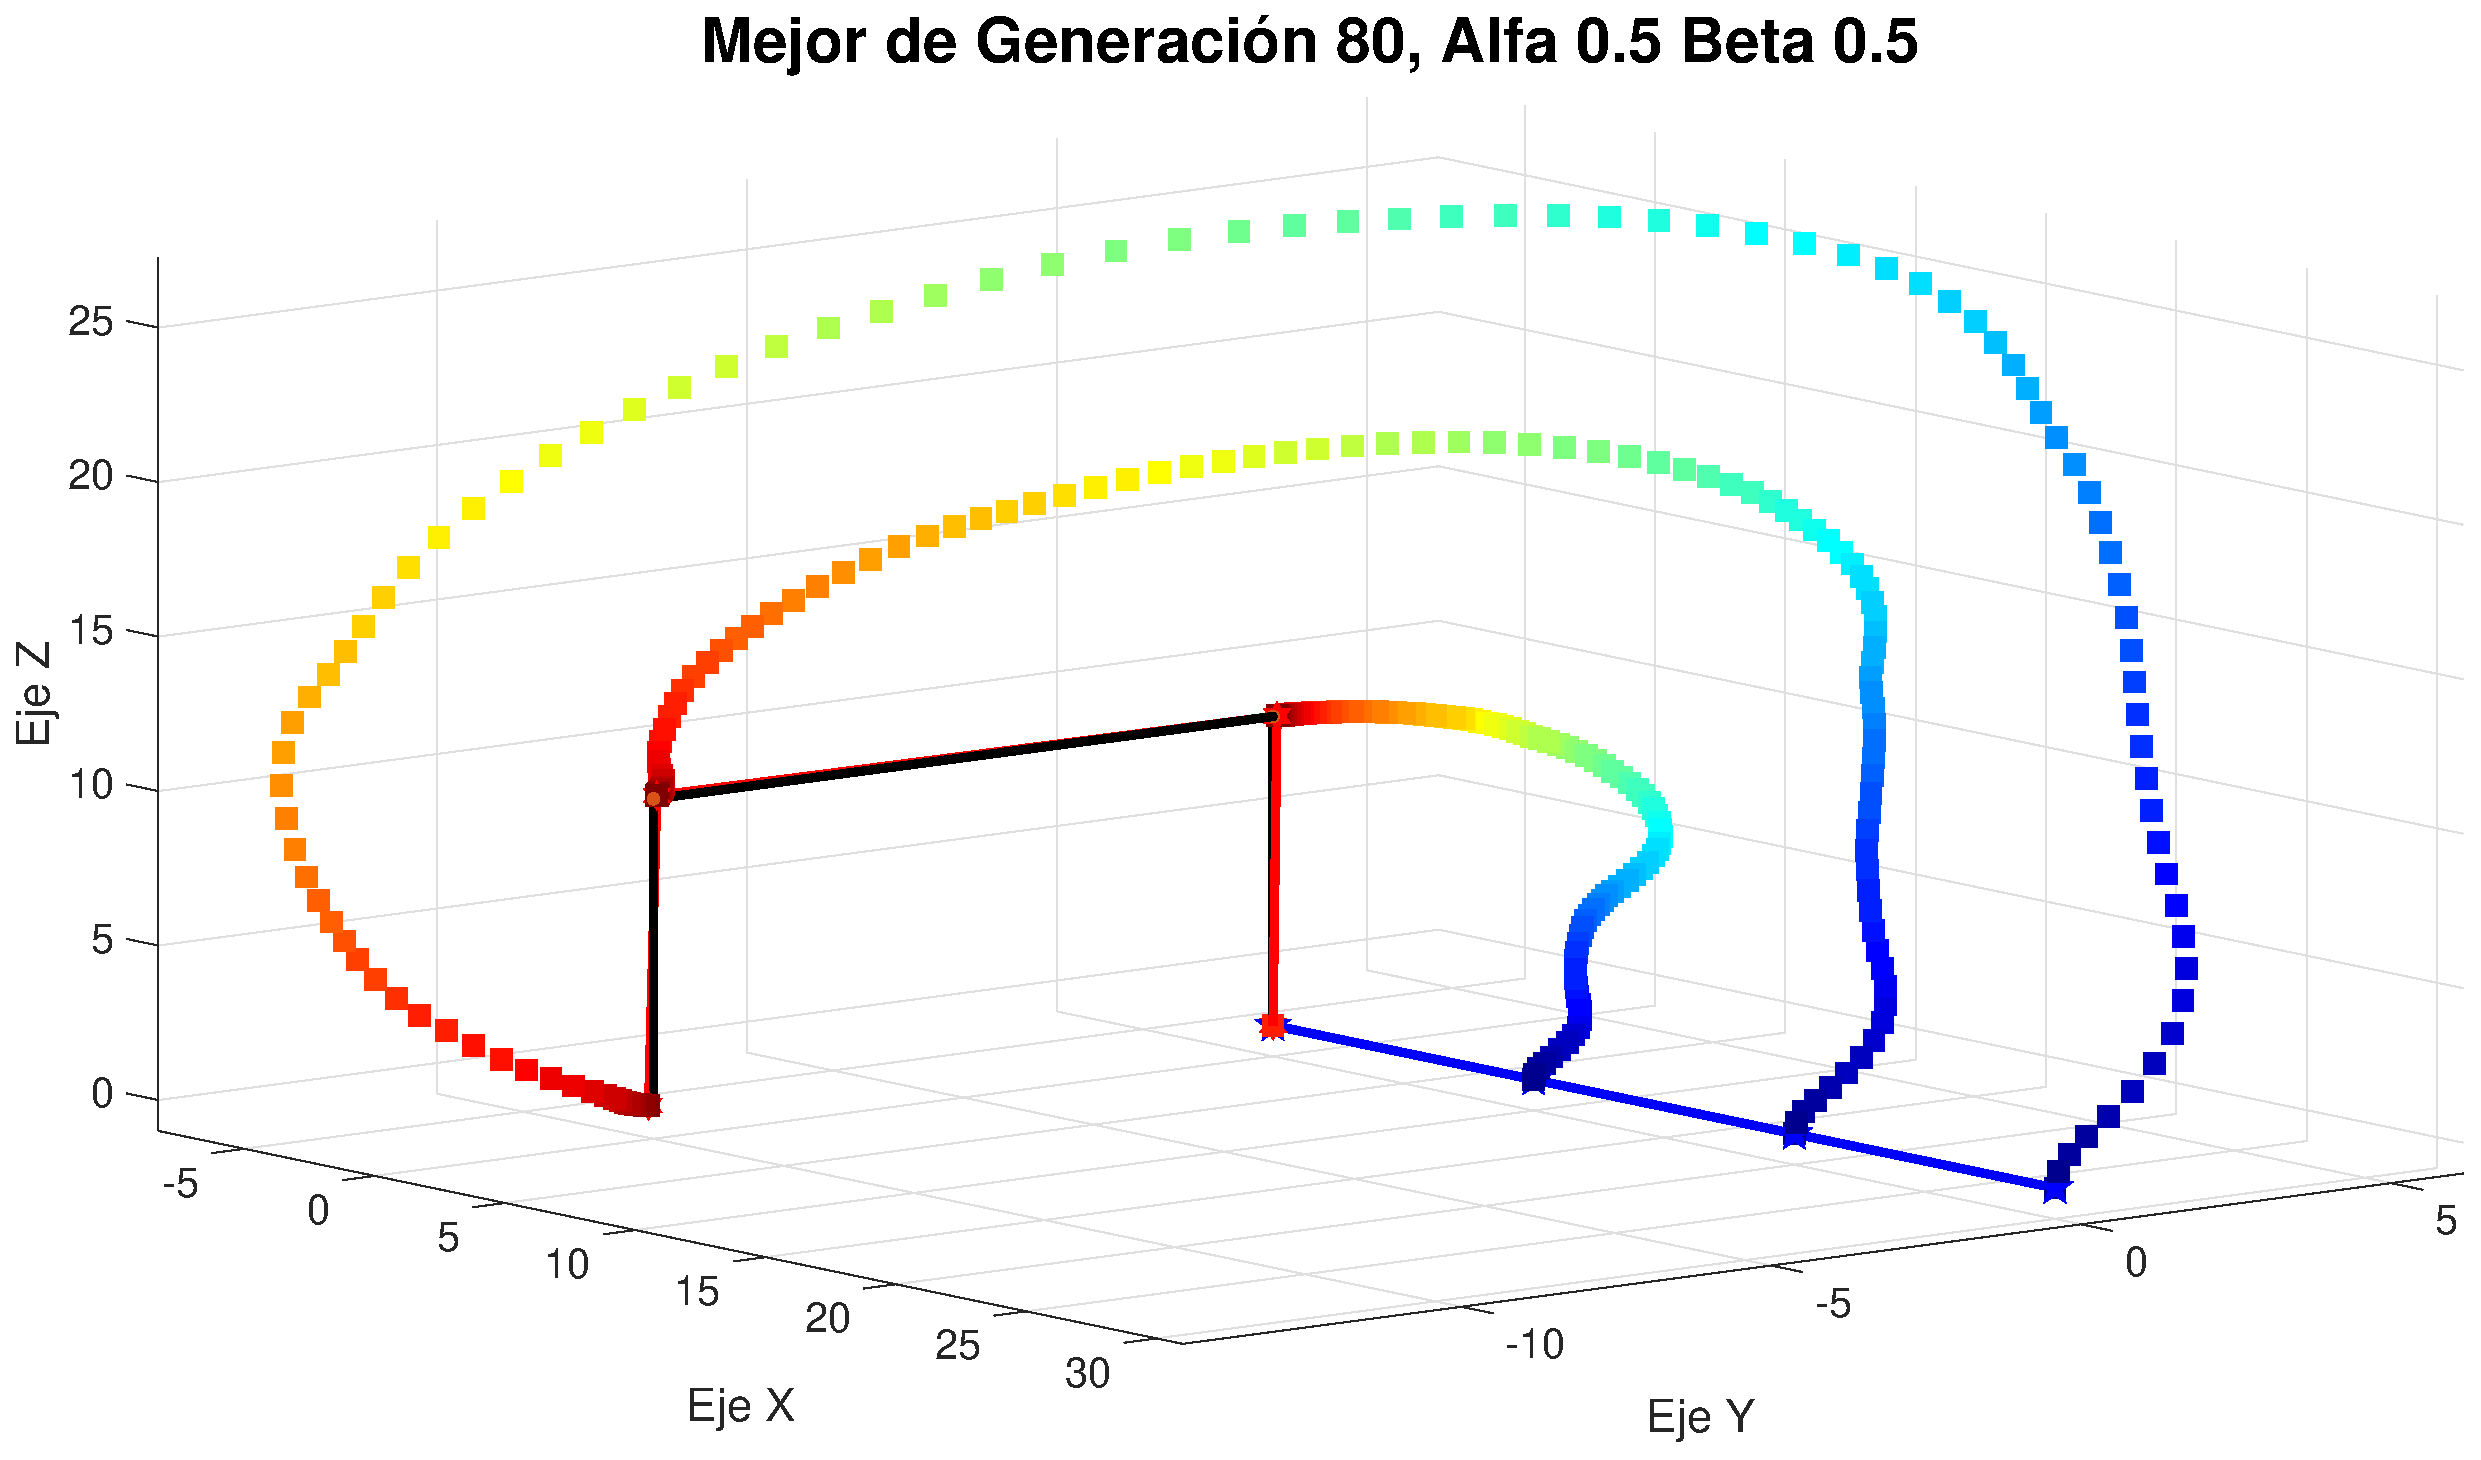
\includegraphics[width=7cm,height=3cm]{imag/versus/MejorSinMutacion.eps}}
\subfigure[Peor trayectoria sin mutación.]{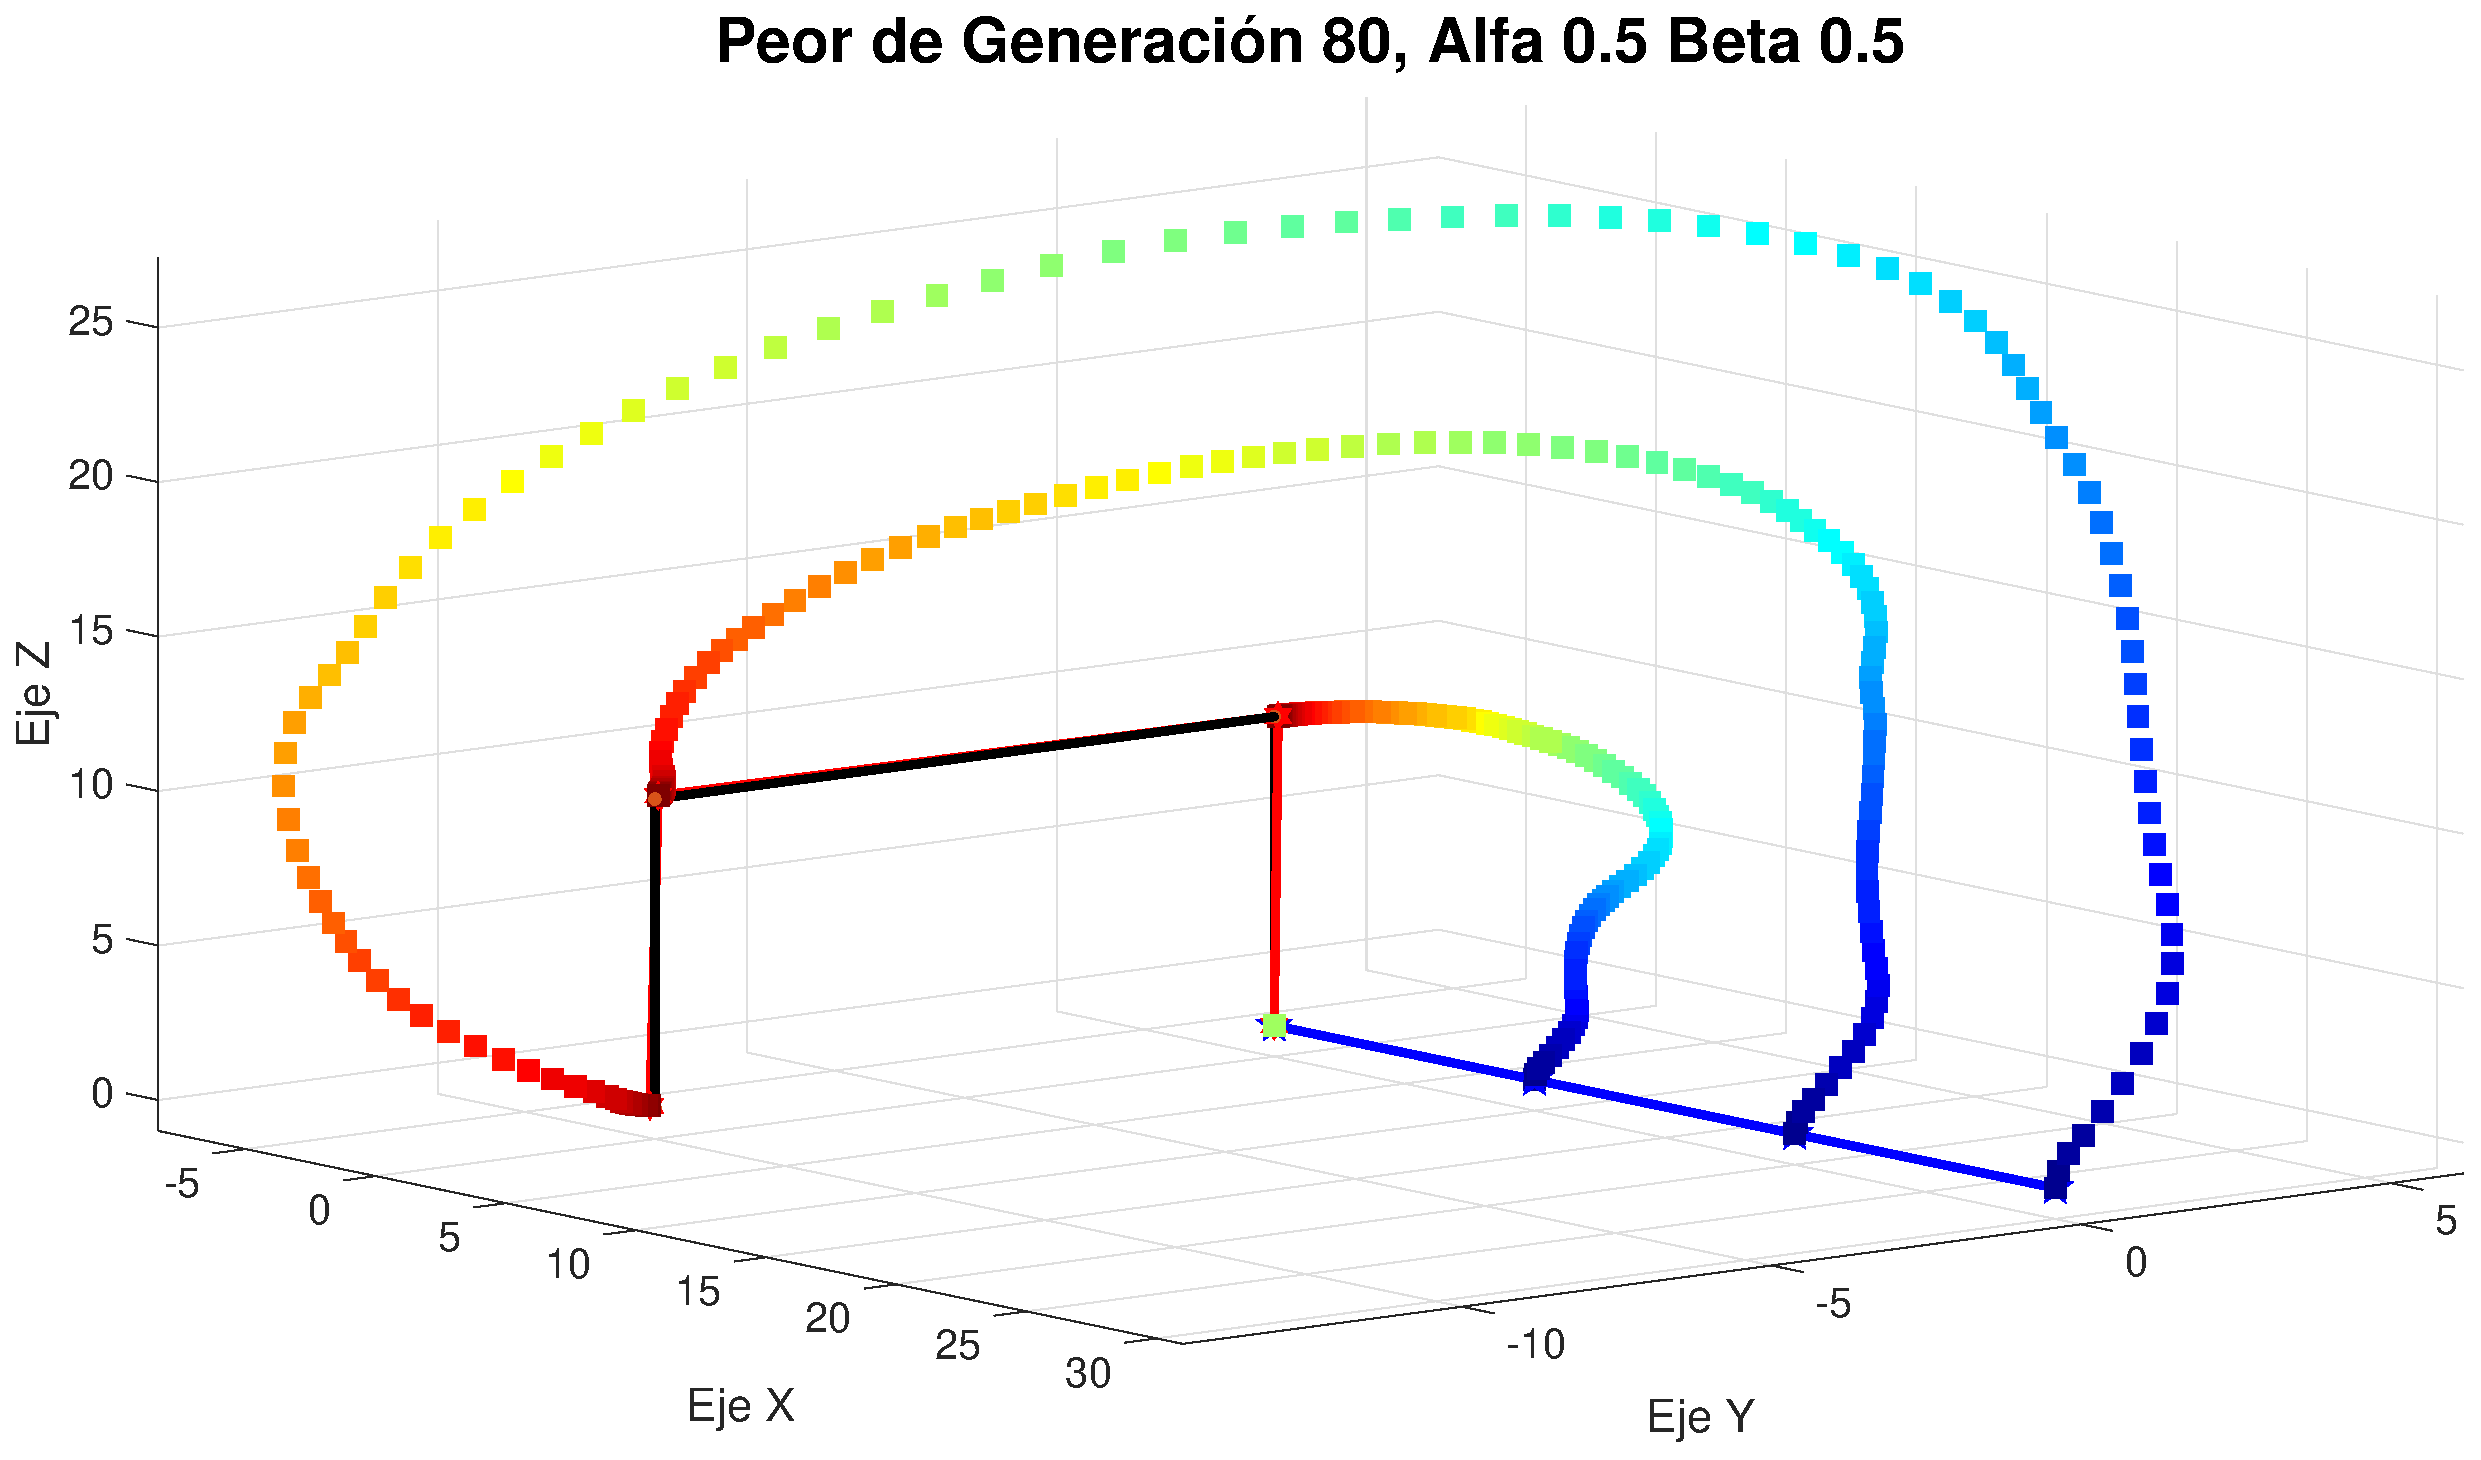
\includegraphics[width=7cm,height=3cm]{imag/versus/PeorSinMutacion.eps}}
\caption{Comparación entre mejores y peores trayectorias para simulaciones con y sin mutación con un $\alpha$: 0.5 y $\beta$: 0.5.}
\label{lalalalalal}
\end{figure}

\newpage
\section{Conclusión}
Como repuesta general del sistema ante las curvas definidas en la evolución de la trayectoria, se logro sintetizar un resultado en el que cada individuo iba mejorando su alcance geométrico hasta el punto objetivo evitando que las muestras se separen demasiado. Por otro lado, se tiene que:
\begin{itemize}
    \item El método para crear los individuos (en este caso: tanh) es crítico para posicionar las muestras de manera consistente. Se debe estudiar en detalle como los crea y como genera la dispersión de los puntos antes de aplicar directamente. Uno de los inconvenientes era que al dejar todo la creación de puntos al azar, el punto inicial se reiniciaba y se convertía en un valor aleatorio, fenómeno que no debiera ocurrir. Esto se soluciono desplazando el punto inicial creado en la primera generación hasta su valor inicial definido por el problema.
    \item Los resultados van mejorando a medida que el fitness va considerando más variables estado en la penalización, por ejemplo, la posición y velocidad. Esto hace que la curva mejor llegue al objetivo y con la menor velocidad posible.
    \item Cuando la evolución de los dato no posee mutación, como es de esperar, se estabiliza en un punto del fitness y de la posición objetivo. Aplicar un porcentaje de mutación minimiza el error de posición final. Sin embargo, para valores muy alto de porcentaje de mutación la solución tiende a oscilar y/o errar.
    \item Si bien la solución final muestra curvas bruscas en la trayectoria, la solución cumple con el objetivo y con el fitness propuesto, llegando al punto final y evitando que la separación entre cada punto sea excesiva, es decir, se disminuye la velocidad.
    \item Cuando se analiza el comportamiento del brazo para diferentes valores de $\alpha$ y $\beta$ se pueden notar leves cambios en la trayectoria impactando principalmente en la separación de las muestras. La llegada del brazo al punto final tiene ciertos margenes de error aún para altos valores de $\alpha$.
\end{itemize}

\newpage
\bibliographystyle{IEEEtran}
\bibliography{biblio}
\end{document} 